\documentclass[letterpaper,12pt,oneside,final]{book}
%%
%%  Gabarit de mémoire de maîtrise ou thèse de doctorat.
%%  Template for dissertations and theses @ Polytechnique Montreal.

%%  Normalement, il n'est pas nécessaire de modifier ce document
%%  sauf pour établir le langage (français ou anglais) et pour changer les noms des 
%%  fichiers à inclure.
%%  Usually, this document needs to be modified only to set up the language (French or English) 
%%  and to change the names of the files to include.
%%
%%  Version: 2018-07-31
%%
%%  Accepte les caractères accentués dans le document (UTF-8).


\makeatletter
\def\bstctlcite{\@ifnextchar[{\@bstctlcite}{\@bstctlcite[@auxout]}}
\def\@bstctlcite[#1]#2{\@bsphack
 \@for\@citeb:=#2\do{%
   \edef\@citeb{\expandafter\@firstofone\@citeb}%
   \if@filesw\immediate\write\csname #1\endcsname{\string\citation{\@citeb}}\fi}%
 \@esphack}
\makeatother

% LA COMMANDE SUIVANTE ÉTABLIT LE LANGAGE DE LA THÈSE : ÉCRIRE french POUR UNE THÈSE EN FRANÇAIS
% THE NEXT COMMAND DETERMINES THE LANGUAGE OF THE THESIS: WRITE english FOR A THESIS IN ENGLISH
\newcommand\Langue{french}            

\usepackage{ifthen}
\usepackage[utf8]{inputenc}
%%
%% Support pour l'anglais et le français (français par défaut).
%\usepackage[cyr]{aeguill}
\usepackage{lmodern}      % Police de caractères plus complète et généralement indistinguable visuellement de la police standard de LaTeX (Computer Modern).
\usepackage[T1]{fontenc}  % Bon encodage des caractères pour qu'Acrobat Reader reconnaisse les accents et les ligatures telles que ffi.

% le langage par défaut est le dernier de la liste, c'est-à-dire français
\ifthenelse{\equal{\Langue}{english}}{
	\usepackage[french,english]{babel}
}{
	\usepackage[english,french]{babel} 
}

%%
%% Charge le module d'affichage graphique.
\usepackage{graphicx}
\usepackage{epstopdf}  % Permet d'utiliser des .eps avec pdfLaTeX.
%%
%% Recherche des images dans les répertoires.
\graphicspath{{./images/}{./dia/}{./gnuplot/}}
%%
%% Un float peut apparaître seulement après sa définition, jamais avant.
\usepackage{flafter,placeins}
%%
%% Utilisation de natbib pour les citations et la bibliographie.
%\usepackage{natbib}
%%
%% Autres packages.
\usepackage{amsmath,color,soulutf8,longtable,colortbl,setspace,xspace,url,pdflscape,cite}
%%
%% Support des acronymes.
\usepackage[nolist]{acronym}
\onehalfspacing                % Interligne 1.5.
%%
%% Définition d'un style de page avec seulement le numéro de page à
%% droite. On s'assure aussi que le style de page par défaut soit
%% d'afficher le numéro de page en haut à droite.
\usepackage{fancyhdr}
\fancypagestyle{pagenumber}{\fancyhf{}\fancyhead[R]{\thepage}}
\renewcommand\headrulewidth{0pt}
\makeatletter
\let\ps@plain=\ps@pagenumber
\makeatother
%%
%% Module qui permet la création des bookmarks dans un fichier PDF.
%\usepackage[dvipdfm]{hyperref}
\usepackage{hyperref}
\usepackage{caption}  % Hyperlien vers la figure plutôt que son titre.
\makeatletter
\providecommand*{\toclevel@compteur}{0}
\makeatother
%%
%% Définitions spécifiques au format de rédaction de Poly.
%% Here we define the Poly formatting.
\RequirePackage[\Langue]{MemoireThese}
%%
%% Définitions spécifiques à l'étudiant.
%% -----------------------------------
%% ---> À MODIFIER PAR L'ETUDIANT / TO BE MODIFIED BY THE STUDENT <---
%% -----------------------------------
%%
%% Commandes qui affichent le titre du document, le nom de l'auteur, etc.
\newcommand\monTitre{Conception, fabrication et test d'une roue Cyr haute performance}
\newcommand\monPrenom{Charlotte}
\newcommand\monNom{Dubost}
\newcommand\monDepartement{génie mécanique}  % Department
\newcommand\maDiscipline{Génie mécanique}
\newcommand\monDiplome{M}        % (M)aîtrise ou (D)octorat / (M)aster or Ph(D)
\newcommand\anneeDepot{2020}    % Year
\newcommand\moisDepot{Juillet}       % Month
\newcommand\monSexe{F}           % "M" ou "F" = Gender
\newcommand\PageGarde{N}         % "O" ou "N" = Yes or No
\newcommand\AnnexesPresentes{O}  % "O" ou "N". Indique si le document comprend des annexes. / If the thesis includes annexes = O or N = No.
\newcommand\mesMotsClef{Cirque,roue,cyr,composites,elasticité}
\usepackage{gensymb}
%%
%%  DEFINITION DU / OF JURY
%%
%%  Pour la définition du jury, les macros suivantes sont definies:
%%  \PresidentJury, \DirecteurRecherche, \CoDirecteurRecherche, \MembreJury, \MembreExterneJury
%%
%%  Toutes les macros prennent 3 paramètres: Sexe (M/F), Nom, Prénom
%%  All the macros have 3 parameters: Sex (M/F), Last name, First name
\newcommand\monJury{\PresidentJury{F}{Nom}{Prenom}\\
\DirecteurRecherche{M}{Gosselin}{Frédérick}\\
\CoDirecteurRecherche{F}{Ross}{Annie}\\
\CoDirecteurRecherche{M}{Therriault}{Daniel}\\
\MembreJury{M}{Nom}{Prénom}\\
\MembreExterneJury{M}{Nom}{Prénom}}


\ifthenelse{\equal{\monDiplome}{M}}{
\newcommand\monSujet{Mémoire de maîtrise}
\newcommand\monDipl{Maîtrise ès sciences appliquées}
}{
\newcommand\monSujet{Thèse de doctorat}
\newcommand\monDipl{Philosophi\ae{} Doctor}
}
%%
%% Informations qui sont stockées dans un fichier PDF.
\hypersetup{
  pdftitle={\monTitre},
  pdfsubject={\monSujet},
  pdfauthor={\monPrenom{} \monNom},
  pdfkeywords={\mesMotsClef},
  bookmarksnumbered,
  pdfstartview={FitV},
  hidelinks,
  linktoc=all
}
%%
%% Il y a un document par chapitre du mémoire.
%%
\begin{document}
\bstctlcite{IEEEexample:BSTcontrol}

%%
%% Page de titre du mémoire.
\frontmatter
% Compte optionellement la page de garde dans la pagination.
\ifthenelse{\equal{\PageGarde}{O}}{\addtocounter{page}{1}}{}
\thispagestyle{empty}%
\begin{center}%
\vspace*{\stretch{0.1}}
\textbf{POLYTECHNIQUE MONTRÉAL}\\
affiliée à l'Université de Montréal\\
\vspace*{\stretch{1}}
\textbf{\monTitre}\\
\vspace*{\stretch{1}}
\textbf{\MakeUppercase{\monPrenom~\monNom}}\\
Département de~{\monDepartement}\\
\vspace*{\stretch{1}}
\ifthenelse{\equal{\monDiplome}{M}}{Mémoire présenté}{Thèse présentée} en vue de l'obtention du diplôme de~\emph{\monDipl}\\
\maDiscipline\\
\vskip 0.4in
\moisDepot~\anneeDepot
\end{center}%
\vspace*{\stretch{1}}
\copyright~\monPrenom~\monNom, \anneeDepot.
%%
%% Identification des membres du jury.
%%
\newpage\thispagestyle{empty}%
\begin{center}%

\vspace*{\stretch{0.1}}
\textbf{POLYTECHNIQUE MONTRÉAL}\\
affiliée à l'Université de Montréal\\
\vspace*{\stretch{2}}
Ce\ifthenelse{\equal{\monDiplome}{M}}{~mémoire intitulé}{tte thèse intitulée} :\\
\vspace*{\stretch{1}}
\textbf{\monTitre}\\
\vspace*{\stretch{1}}
présenté\ifthenelse{\equal{\monDiplome}{M}}{}{e}
par~\textbf{\mbox{\monPrenom~\MakeUppercase{\monNom}}}\\
en vue de l'obtention du diplôme de~\emph{\mbox{\monDipl}}\\
a été dûment accepté\ifthenelse{\equal{\monDiplome}{M}}{}{e} par le jury d'examen constitué de :\end{center}
\vspace*{\stretch{2}}
\monJury
%%
\pagestyle{pagenumber}%
%% Dédicace
%%
%% La dédicace est un hommage que l'auteur souhaite
%% rendre à une ou plusieurs personnes de son choix.
%%
\ifthenelse{\equal{\Langue}{english}}{
	\chapter*{DEDICATION}\thispagestyle{headings}
	\addcontentsline{toc}{compteur}{DEDICATION}
}{
	\chapter*{DÉDICACE}\thispagestyle{headings}
	\addcontentsline{toc}{compteur}{DÉDICACE}
}

\begin{flushright}
  \itshape
  A ceux qui mettent leurs connaissances et compétences au service de l'art, et à ceux qui cherchent un moyen de le faire. 
  \ldots
\end{flushright}
          % Dédicace du document.
% Remerciements / Acknowledgements
%
%  Grâce aux remerciements, l'auteur attire l'attention du lecteur
% sur l'aide que certaines personnes lui ont apportée, sur leurs
% conseils ou sur toute autre forme de contribution lors de la
% réalisation de son mémoire. Le cas échéant, c'est dans cette section
% que le candidat doit témoigner sa reconnaissance à son directeur de
% recherche, aux organismes dispensateurs de subventions ou aux
% entreprises qui lui ont accordé des bourses ou des fonds de
% recherche.
\ifthenelse{\equal{\Langue}{english}}{
	\chapter*{ACKNOWLEDGEMENTS}\thispagestyle{headings}
	\addcontentsline{toc}{compteur}{ACKNOWLEDGEMENTS}
}{
	\chapter*{REMERCIEMENTS}\thispagestyle{headings}
	\addcontentsline{toc}{compteur}{REMERCIEMENTS}
}
%
Merci à mes directeurs de recherche, Frédérick Gosselin, Annie Ross et Daniel Therriault pour l'énergie et le temps qu'ils ont accordé à l'accompagnement de ce projet ainsi que pour leur vivacité d'esprit et l'excellence de leurs expertises dont j'ai eu la chance de bénéficier. \\\\
Merci à Marion Cossin pour son soutien, ses précieux conseils et son appui au sein de l'Ecole Nationale de Cirque de Montréal dès le début du projet.\\\\
Merci à toute l'équipe de l'Ecole Nationale de Cirque pour sa collaboration.
     % Remerciements.
% Résumé du mémoire.
%
\chapter*{RÉSUMÉ}\thispagestyle{headings}
\addcontentsline{toc}{compteur}{RÉSUMÉ}

La roue Cyr est un agrès de cirque composé d’une roue métallique à la géométrie torique dont le diamètre avoisine la hauteur de l’utilisateur et dont le poids varie de 10kg à 20kg. L’utilisateur se place au centre de la roue, s’y agrippe et effectue des figures acrobatiques tout en tournant. Ceci fait du poids et de la rigidité des facteurs déterminants pour la performance de l’utilisateur. Depuis son invention cet agrès a été revisité plusieurs fois par des artistes et des fabricants d’équipement de cirque. En particulier, depuis que l’utilisation de matériaux avancés (comme la fibre de carbone) est devenue populaire pour les équipements sportifs, et qu’elle commence à être adopté par certains fabricants pour les mats et les portiques, la communauté circassienne manifeste de l'intérêt pour les possibilités nouvelles qu’une roue Cyr plus légère et plus flexible pourrait apporter. La géométrie torique d’une roue Cyr rend sa fabrication plus compliquée et le prototypage plus couteux, parmi les projets de roue Cyr en matériaux composites, aucun n’a été mené à bien, pour cause manque de moyens où d’absence de modélisation théorique. En outre, développer une modélisation dynamique de la roue Cyr (dont le mouvement est similaire à celui du disque d’Euler) nécessite de se plonger dans une étude approfondie.
Le but de ce projet est donc de déterminer de quelle manière l’utilisation de matériaux composites pour la fabrication d’une roue Cyr enrichira la discipline, aussi bien en termes de possibilités acrobatiques que de jeu de scène, ainsi que d’identifier des propriétés mécaniques et géométries optimisées correspondant aux mouvements et aux efforts exercés sur une roue Cyr.



Le déroulement du projet est basé sur la méthodologie suivante:
\begin{itemize}
\item Étude théorique : Développement d’un modèle mathématique des mouvements caractéristiques de la roue Cyr et du stockage d’énergie, des sauts et rebonds. Une fois que le modèle est établi, caractérisation des paramètres géométriques et mécaniques déterminants ainsi que de leur influence. Développement d’une analyse adimensionnelle et d’une loi d’échelle.
\item Étude numérique : développement d’un modèle numérique des mouvements de la roue Cyr en utilisant Python.
\item Preuve de concept : Une fois que les propriétés optimales ont été déterminées imprimer en 3D une petite portion de la roue, de même rayon de courbure, avec le matériau correspondant. Une fois que cette portion est testée et validée, imprimer un modèle réduit et le tester adéquatement à l’aide de la loi d’échelle déterminée à l’étude théorique.
\item Prototypage à l’échelle 1
\item Test du prototype : En partenariat avec l’École Nationale de Cirque de Montréal.
\end{itemize}

Le projet contribue à l’avancement des connaissances dans différents domaines et pour des communautés diversifiées : en plus de compléter certaines recherches concernant le disque d’Euler, ou plus globalement les disques et les tores en rotation ou les anneaux élastiques, ce qui fait l’originalité et l’importance du projet réside dans l’apport de nouvelles connaissances à la communauté circassienne : les fabricants d’équipement de cirque auront une réponse concernant l’intérêt de la fabrication de roue Cyr en matériaux composites, ainsi qu’un exemple de procédé de fabrication et, (surtout !) pour les artistes et metteurs en scène la discipline se verra enrichie par de nouvelles possibilités et de nouvelles opportunités de création.

      % Résumé du sujet en français.
% Abstract
%
% Résumé de la recherche écrit en anglais sans être
% une traduction mot à mot du résumé écrit en français.

\chapter*{ABSTRACT}\thispagestyle{headings}
\addcontentsline{toc}{compteur}{ABSTRACT}
%

The Cyr Wheel is a circus apparatus consisting of a 2 meters diameter (size may vary with the height of the user) ring made of steel or aluminum, with a weight varying between 10kg and 20kg. The user stands inside the wheel and performs acrobatic tricks while spinning. This utilization makes the weight, rigidity and geometry determinant influence parameters for the way the user will perform on the wheel. Since its invention in 1996 it has been revisited several times by circus artists and manufacturers, and especially with the utilization of advanced materials for sport equipment spreading to circus structures (such as poles and gantries), the circus community shows interest for the possibilities that a lighter, more flexible Cyr wheel could bring (like jumping and bouncing with the wheel, for instance). The fact that a Cyr wheel is made of curved elements leads to a significant increase in terms of fabrication costs, and none of the Cyr wheel projects involving new composite materials has been completed to this day, mostly because of a lack of means, and the fact that it is too expensive to get to the right prototype by the ‘trial and error’ method. On the other hand, developing a theoretical model of the dynamics of Cyr wheel is a complex task which requires an in-depth study since its motion can be linked to the Euler’s disk model. 
For now, advances on this question consist in trials of prototypes manufactured with no prior theoretical studies which resulted in a lack of optimization and unsuitable material choices leading to failure when tested.\\ 

To this day there aren’t any scientific publications specific to the Cyr wheel dynamics or the use of composite materials for circus structures. Nevertheless, Euler’s disk and spinning coins have been widely studied by the scientific community due to the chaotic aspect of their motion in its terminal stage as well as the influence of friction and air viscosity on its behavior. The mathematical model developed to study this problem provide a basis that will be adapted the dimension, shape and use of the Cyr wheel. The ability to jump with the Cyr wheel being a determinant aspect of the study, the model developed by Yang and Kim about energy storage in elastic rings will also be used as a basis an adapted to the scale and problematics specific to a Cyr wheel.\\

Carrying out the study of a composite Cyr wheel from its design to the test and validation of a prototype requires to combine at the same time practical knowledge of the apparatus, theoretical knowledge about composite materials, 3D printing processes and dynamics of Euler’s disk-like motions, as well as mastery of numerical modelling and large scale composite 3D printing equipment. These conditions are hard to reunite at once, which explains why, contrary to other circus apparatuses, the question of the use of composite materials for Cyr wheel manufacturing has not been solved yet and why no scientific publication has been released on this subject. Answering this problematic represents a significant evolution of the discipline of Cyr wheel and of the manufacturing of this apparatus. On top of that, it will allow to bring quantitative answers to multiple questions that have only be tackled intuitively until then.\\
The general objective of this study is to estimate the mechanical properties and geometry that will allow to optimize and diversify the use of a Cyr wheel, choose a corresponding material to 3D print the Cyr wheel in, print a real size prototype and experiment on the new acrobatic possibilities of this new apparatus.

The guidelines of the project are the following research questions:
\begin{itemize}
\item What would be the optimal material properties (Young modulus, density) and geometry that would expand the acrobatic possibilities of a Cyr wheel ? 
\item	How would this circus discipline evolve with a corresponding Cyr wheel made out of a high-performance optimized material ? 
\end{itemize}


The project is based on the following hypothesis:
\newline
Developing a Cyr wheel with a rigidity and a weight different from the existing ones will significantly contribute to the evolution of the discipline.\\
This hypothesis will be refuted if the new acrobatic tricks that we suppose this new type of Cyr wheel will allow are too demanding (physically or in terms of skills) and can’t be achieved by a professional Cyr wheel performer, even with some practice time.\\

Justification of the originality: Considering the dynamics of a spinning Cyr wheel with a performer, adding elastic properties and a lighter weight sounds promising and has been tried several times, but never achieved.\\
Success criteria: a successful contribution would consist in advances in the theoretical knowledge of Cyr wheel, by quantitatively answering problematics raised by the circus community, evolution of the discipline by expanding the acrobatic possibilities of this apparatus and providing answers concerning the interest of the introduction of composite materials for Cyr wheels to manufacturers.\\

The project will be carried out with the following methodology:

\begin{enumerate}
\item Theoretical study:
develop a mathematical model of Cyr wheel motions and of energy storage, jumping and bouncing. Once the model is established, identify the parameters of significant influence among material properties and geometry parameters (Young modulus, density, moment of inertia, size of diameter…). Study the scalability and develop an dimensionless analysis.

\item Numerical study:
develop a numerical model of Cyr wheel motions, study the dynamic stability and energy storage capability. Quantify the influence of the identified parameters by studying the impact of their variation on the motion.

\item Proof of concept:
once the optimal properties of the material are estimated thanks to the two previous phases, develop a corresponding composite material and 3D print a small part of the wheel with the same radius of curvature than the real-size one. Once it is tested and validated, print a small size prototype and test it applying appropriate strength estimated with the scalability study.

\item Real size prototyping:
3D-print the final prototype: a real size Cyr wheel made out of the optimized high performance composite material previously defined

\item Test of the prototype:
validate that the chosen material is appropriate.
Explore the news acrobatic possibilities provided by the prototype.

\end{enumerate}


The impacts and benefits of the project are the following:
\begin{itemize}
\item Carrying out this study will allow circus equipment manufacturers to further the reflection and conclude on the pros and cons of adding composite Cyr will to their current offer.
\item Developing a numerical model of Cyr wheel motions will allow to quantify the influence of different parameters such as rigidity, density and geometry on the performance of the user. This will bring an answer to problematics left unanswered until now such as the ones put forward by the research department of Montreal National Circus School (ideal user’s weight/ Cyr wheel weight ratio, ideal user’s height, Cyr wheel diameter ratio) 
\item The resulting research article will provide a basis for further investigation about the Cyr wheel, since no publication has been released on this topic to this day.
\item On a broader perspective, this study will be a contribution to advances in the research on sporting equipment involving circular shapes and problematics of lightness and flexibility.

\end{itemize}
          % Résumé du sujet en anglais.

{\setlength{\parskip}{0pt}
%%
%% Table des matières.
\ifthenelse{\equal{\Langue}{english}}{
	\renewcommand\contentsname{TABLE OF CONTENTS}
}{
	\renewcommand\contentsname{TABLE DES MATIÈRES}
}
\tableofcontents
%%
%% Liste des tableaux.
\ifthenelse{\equal{\Langue}{english}}{
	\renewcommand\listtablename{LIST OF TABLES}
}{
	\renewcommand\listtablename{LISTE DES TABLEAUX}
}\listoftables
%%
%% Table des figures.
\ifthenelse{\equal{\Langue}{english}}{
	\renewcommand\listfigurename{LIST OF FIGURES}
}{
	\renewcommand\listfigurename{LISTE DES FIGURES}
}\listoffigures
%%
%% Liste des annexes au besoin.
}

% Liste des sigles et abbréviations / List of acronyms and abbreviations
\ifthenelse{\equal{\Langue}{english}}{
	\newcommand\abbrevname{LIST OF SYMBOLS AND ACRONYMS}
}{
	\newcommand\abbrevname{LISTE DES SIGLES ET ABRÉVIATIONS}
}
\chapter*{\abbrevname}
\addcontentsline{toc}{compteur}{\abbrevname}
\pagestyle{pagenumber}
%
\begin{acronym}
  \acro{ENC}{Ecole Nationale de Cirque}
  \acro{CNAC}{Centre National des Arts du Cirque}
  \acro{FEDEC}{Fédération Européenne Des Ecoles de Cirque professionnelles}
\end{acronym}
%
\begin{longtable}{lp{5in}}
ENC       & Ecole Nationale de Cirque\\
CNAC       & Centre National des Arts du Cirque\\
FEDEC       & Fédération Européenne Des Ecoles de Cirque professionnelles\\
\end{longtable}

       % Liste des sigles et abréviations.
\ifthenelse{\equal{\AnnexesPresentes}{O}}{\listofappendices}{}
\mainmatter
% Dans l'introduction, on présente le problème étudié et les buts
% poursuivis. L'introduction permet de faire connaître le cadre de la
% recherche et d'en préciser le domaine d'application. Elle fournit
% les précisions nécessaires en ce qui concerne le contexte de
% réalisation de la recherche, l'approche envisagée, l'évolution de
% la réalisation. En fait, l'introduction présente au lecteur ce
% qu'il doit savoir pour comprendre la recherche et en connaître la
% portée.

\Chapter{INTRODUCTION}\label{sec:Introduction}  % 10-12 lignes pour introduire le sujet.

\\
Support d'acrobatie, entrainant le corps de l'utilisateur qui s'y accroche dans un mouvement de rotation, mais pouvant aussi bien être manipulée par ce dernier, la roue Cyr se place à mi-chemin entre les disciplines acrobatiques, les disciplines d'équilibrisme et la manipulation d'objet. La réalisation de figures acrobatiques repose sur un équiibre dynamique continuel entre la roue et le corps de l'utilisateur: ce dernier influe sur le mouvement de la roue, tout en modulant le rythme et la force qu'il applique en fonction des caractéristiques de la roue (sa masse, son inertie, sa géométrie). Un changement dans ces caractéristiques rend ainsi nécessaire l'adaptation de l'artiste à une variation du mouvement. La popularité croissante de l'utilisation de matériaux composites pour la fabrication d'équipement de cirque comme les mats ou les portiques éveille l'intérêt de la communauté circassienne sur les possibilités nouvelles qu'une roue Cyr faite d'un tel matériau peut apporter. L'enjeu est double: le procédé de fabrication offrant un éventail de possibilités géométriques inaccessibles avec les métaux ainsi qu'un choix des propriétés mécaniques beaucoup plus large, on y voit une occasion d'optimiser les mouvements déjà existants mais aussi d'inventer de nouvelles figures avec une roue Cyr faite d'un matériau dont les propriétés élastiques permettent, par exemple, de sauter avec la roue.
%%
%%  CONCEPTS DE BASE / BASIC CONCEPTS
%%
\section{Définitions et concepts de base}  % environ 2-3 pages



\subsection{Définitions}
\paragraph{Circassien(ne):} relatif au cirque 
\paragraph{Agrès de cirque:} équipement nécessaire à la pratique d'une discipline circassienne. Exemples: la roue Cyr, le trapèze, le tissu aérien, les cannes d'équilibre, le mat chinois...
\paragraph{Disque d'Euler:} disque ayant un mouvement de rotation similaire à celui d'une pièce qu'on fait tourner sur une surface plane. Lorsque son mouvement entre en phase terminale sa vitesse de rotation augmente de façon impressionnante, ce qui lui a valu de devenir un jouet éducatif, mais aussi de faire l'objet de nombreuses publications scientifiques. Son mouvement est similaire à un des mouvements caractéristiques de la roue Cyr.


\subsection{Historique de la roue Cyr}
La roue Cyr que l'on retrouve dans les spectacles de cirque contemporains doit son  nom à Daniel Cyr, qui fabriqua sa première roue en 1996 \cite{Inertie}. A cette dernière, faite en une seule pièce d'acier recouverte d'un revêtement en PVC afin d'améliorer l'adhérence avec le sol, succéda rapidement  une roue Cyr démontable en plusieurs parties. La première apparition marquante de la roue Cyr sur la scène circassienne eut lieu en 1998 dans un spectacle du Cirque Eloize, dont Daniel Cyr est le co-fondateur. Une médaille d'argent remportée en 2003 par ce dernier au Festival Mondial du Cirque de Demain acheva d'assoir la popularité de ce nouvel agrès dans le secteur du cirque, mais également en tant que sport.\\
Cependant l'idée d'une roue à la géométrie torique dont le diamètre avoisine la taille humaine remonte bien avant la création de Daniel Cyr \cite{Inertiehist,gymmedia,howstuffwork}. En effet, plusieurs agrès d'apparence similaire à celle de la roue Cyr ont fait leur apparition du côté de l'Allemagne dès le début du vingtième siècle. On remarquera en particulier l'Einrefen, inventé en 1930 par Adalbert von Rekowski, qui diffère de la roue Cyr par des poignées intérieures pour les mains et les pieds. \\
Depuis, la roue Cyr continue d'évoluer, comme le montrent les agrès dérivés présentés à la fin du manuel de la FEDEC (Fédération Européenne Des Ecoles de Cirque professionnelles) \cite{Fedec2011}. Les procédés de fabrication se sont eux aussi affinés \cite{corbin}, et les roues Cyr lumieuses programmables ont vu le jour.\\
La fabrication en matériaux composites se présente aujourd'hui comme l'étape suivante dans l'évolution de l'agrès.

\subsection{Les figures de roue Cyr}
Nous présentons ici les figures de roue Cyr constituant la base principale de la discipline. Ces dernières, ainsi que d'autres figures plus approfondies sont détaillées dans le manuel de la FEDEC \cite{Fedec2011}
\subsubsection{La valse (ou pas de base)}
Le corps est positionné de façon symétrique, avec bras et jambes chacun inclinés à 45\degree de la verticale. L'utilisateur initie la rotation d'une poussée du pied puis accompagne le mouvement de la roue en utilisant le tranfert de son poids, tirant et poussant successivement la roue dans le sens de la rotation.\\
Ce mouvement se décline en plusieurs variations en ajoutant par exemple un lacher de pieds, qui avec un arc de cercle de la jambe devient un arabesque, ou encore en l'exécutant à une seule main ou mains croisées, en serrant et croisant les jambes ou en les écartant jusqu'au grand écart latéral. Cette figure s'exécute aussi avec un pied placé sur la roue au niveau de la tête, en grand écart facial. On peut aussi varier en jouant avec la position du corps: corps de profil, dans le plan de la roue, arqué vers l'intérieur, tendu vers l'extérieur...

\subsubsection{Les tours}
Dissociation du mouvement: la roue tourne mais pas le corps. Ce type de figure peut être exécuté en effectuant un demi-tour, un tour complet, ou même un tour en suspension avec l'utilisateur suspendu à la roue par une main.

\subsubsection{Les vrilles}
Dissociation inverse, le corps tourne dans le reférentiel de la roue. De même ce type de figure se décline en diverses sortes de demi vrilles et en vrille complète en suspension.

\subsubsection{Les suspensions}
Comme l'indique le nom, les pieds ne sont pas sur la roue. On peut par exemple exécuter la valse en suspension, sans les pieds, ou simplement prendre de l'élan puis lacher les pieds et adopter une position groupée en tournant sur place, ce qui a pour effet d'augmenter la vitesse de rotation. Il est possible de se suspendre par une ou deux mains, par les coudes, les bras tendus ou fléchis. La suspension est la base de la figure du Superman: corps gainé, jambes tendues vers l'extérieur de la roue.

\subsubsection{Le drapeau}
La roue n'est tenue que par la main et le pied d'un même côté. La rotation est alimentée en poussant et tirant avec la main et le pied restant, tout en tendant puis groupant successivement la main et le pied lachés.

\subsubsection{Les sauts}
La roue tourne sur elle même, l'utilisateur saute et prend appui come il le souhaite, bras tendus, pliés, ou même en position assise sur la roue. Il peut ensuite atterrir sur le sol ou directement sur la roue.

\subsubsection{Le corner ou inclinaison horizontale}
L'utilisateur se décale sur un côté de la roue jambes serrées, prend appui jambes fléchies puis plonge vers le sol, jambes tendues le corps se retrouve en position horizontale pour un demi tour. Cette figure peut se réaliser en lachant un bras, un pied, ou un bras et un pied simultanément.

\subsubsection{Le saut de mains}
L'utilisateur pousse la roue vers le sol avec une main, accompagne le renversement avec son poids, ouvre les doigts quand sa main arrive au niveau du sol puis la tire au dessus de sa tête et la pousse avec ses jambes afin de revenir à l'endroit. Cette figure s'exécute en avant, en arrière, en position de profil, à une jambe.

\subsubsection{La roue}
L'utilisateur exécute une roue classique tout en étant dans la roue au moyen de transferts de poids. Il est possible de réaliser cette figure en enchainant plusieurs roues le long d'une trajectoire circulaire, ou bien d'une ligne droite. Il est possible de la combiner avec d'autres figures et changements de directions et d'enchainer ainsi plusieurs roues dans des sens différents.

\subsubsection{La pièce}
Ce mouvement est semblable à la rotation d'une pièce de monnaie (ou du disque d'Euler) dans la phase terminale du mouvement. L'utilisateur, gainé, ouvre sucessivement les doigts pour ne pas les écraser lorsque ses mains arrivent au niveau du sol, et transfere son poids pour accompagner le mouvement et l'alimenter aussi longtemps qu'il le souhaite. Cette figure peut s'exécuter à différentes hauteurs du sol, plus la pièce est basse, plus la vitesse sera élevée. On peut aussi la réaliser à l'envers, le corps arqué (pièce dorsale).

\clearpage

%%
%lt% anément eELEMENTt chent la roue simuS DE LA PROBLEMATIQUE
%%
\section{Problématique}  % environ 3 pages
La création d'une roue Cyr en matériaux composites, aux propriétés différentes de celles qui roues Cyr métalliques, qui permettra d'enrichir la discipline de nouvelles figures se trouve au carrefour de la science, de la technique acrobatique et de l'art. Ceci nécessite de réunir des expertises issues de ces différents domaines, couplés à des moyens de fabrication adéquats. La problématique peut donc se découper selon les trois étapes caractéristiques du projet.

\subsection{Conception}
Il s'agit de déterminer quels paramètres parmi les propriétés mécaniques du matériau et la géométrie de la roue Cyr influencent de manière notable les mouvements de cette dernière, puis de caractériser cette influence quantitativement. \\ 
A cet effet des modèles théoriques de deux mouvements caractéristiques ont été développés:
\begin{itemize}
    \item Le saut (la possibilité d’intégrer des sauts aux figures de roue Cyr déjà existante étant une des lignes directrices du projet): la roue est compressée par l'exercice d'une force dont l’axe coincide avec le diamètre, puis relâchée. Une part de l’énergie élastique stockée est convertie en saut. 
    \item Le mouvement correspondant à celui d’une pièce de monnaie qui roule sur sa tranche en décrivant des cercles, puis entre en phase terminale avant de tomber à plat sur le sol.
\end{itemize}

En se basant sur chacun des modèles théoriques correspondants, l’objectif est de déterminer séparément les paramètres géométriques et mécaniques qui :
\begin{itemize}
    \item  permettent à l’utilisateur de sauter le plus haut possible avec la roue.
    \item permettent d’optimiser le mouvement similaire à celui de la pièce de monnaie décrit ci-dessus en termes de stabilité dynamique.
    \item conduisent au meilleur compromis entre les deux réponses aux questions précédentes.
\end{itemize}


Parallèlement, il est indispensable d’étudier les contraintes et déformations dans la roue et plus particulièrement celles dues à l’impact avec le sol lors des sauts afin d’identifier des zones de design, qui garantissent que cette dernière ne sera pas endommagée.

\subsection{Fabrication}
Il s’agit de compléter l’étude théorique issue de la phase de conception par une utilisation adaptée de l’impression 3D. En utilisant les technologies existantes et disponibles pour le projet, comment imprimer un tore d’un diamètre avoisinant les deux mètres ? Comment assurer des propriétés conformes à celles déterminées par les modèles théoriques établis au préalable ? 

\begin{figure}[htb]
\centering
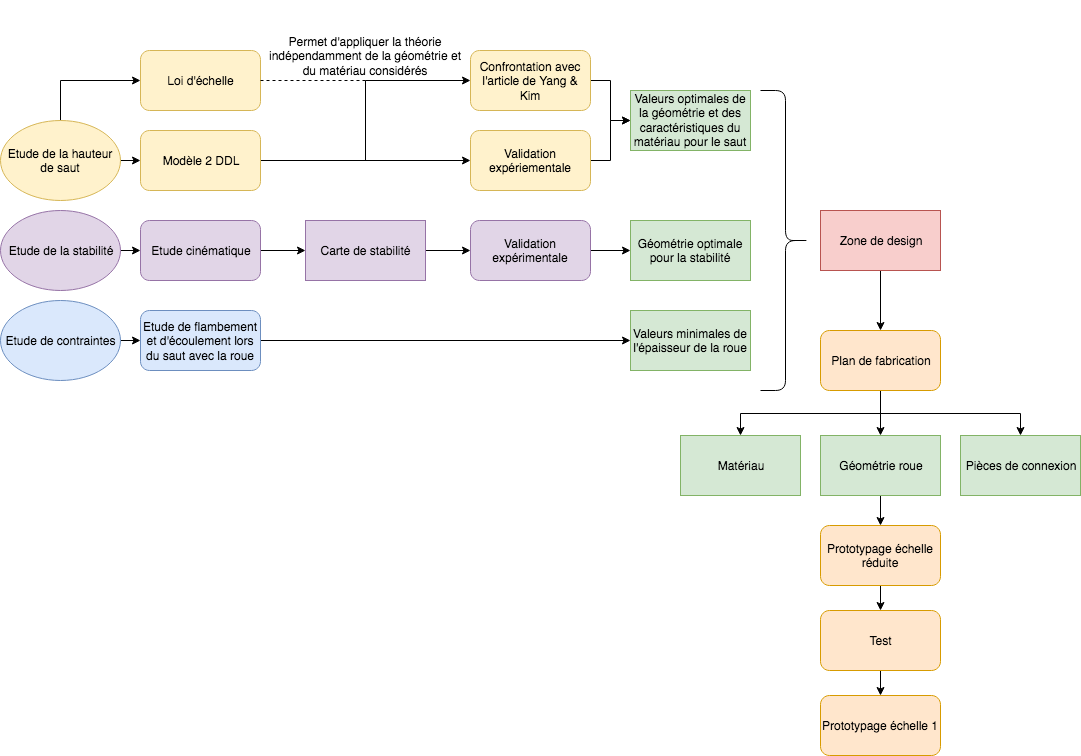
\includegraphics[width=7in]{images_autres/flowchart.png}
\caption{Flowchart résumant les étapes de conception et de fabrication de la roue.}
\label{fig:flowchart}
\end{figure}

\subsection{Tests}
Malgré la popularité du sujet au sein de la communauté circassienne et des pratiquants de roue Cyr, la roue en matériaux composites ne figure pas parmi les offres des fabricants d’équipement de cirque. Ces dernières sont en partie influencées par le fait qu’il y ait un flou, une difficulté à estimer concrètement ce qu’apporterait une telle roue Cyr et donc si les individus adeptes de la discipline seraient prêts à acquérir une roue Cyr composite, pour un prix bien supérieur à ceux des roues métalliques. En effet, leur fabrication nécessite un investissement conséquent qui ne peut être fait sans avoir de certitude sur sa rentabilité. Une phase de recherche artistique menée avec le prototype à l’échelle 1 imprimé et fonctionnel et en collaboration avec des artistes de roue Cyr de haut niveau, permettra de lever le voile sur les nouvelles possibilités introduites par une roue Cyr composite, aussi bien en termes d'acrobaties que de jeu de scène, ainsi que sur la réaction de la communauté et des pratiquants, ce qui permettra aux fabricants d'évaluer plus clairement si une véritable demande peut exister.\\
En outre, plusieurs artistes de roue Cyr ont déjà tenté d'approcher ces nouvelles possibilités, avec des roues Cyr fabriquées de manière artisanales dans des matériaux plus légers ou plus flexibles (par exemple une roue Cyr en osier a été fabriquée par des élèves au Centre National des Arts du Cirque (CNAC) en France)
cependant ces projets d'expérimentation n'ont pu être menés à terme, les roues se retrouvant rapidement endommagées et hors service. Ceci s'explique par le manque de moyens et de temps à consacrer à une étude préalable méthodique et approfondie rassemblant des expertises diverses et des moyens de fabrication adéquats, ainsi qu'une maitrise des procédés de fabrication additive. Fournir un prototype fonctionnel et solide permettra à ces artistes de continuer et d'approfondir leur recherche dans la sécurité, au terme de quoi la discipline pourrait prendre un nouveau tournant.\\


% On veut éviter que la figure et le tableau soient placés au-delà de la section courante.
\FloatBarrier


%%
%% OBJECTIFS DE RECHERCHE / RESEARCH OBJECTIVES
%%
\section{Objectifs de recherche}  % 0.5 page
\subsection{Objectif global}
L'objectif global de ce projet de recherche est de parvenir à la conception d’un prototype de roue Cyr haute performance aux propriétés élastiques, imprimé en 3D à partir d’un matériau optimisé, puis tester avec des artistes de haut niveau les nouvelles possibilités offertes par cet agrès

\subsection{Objectifs spécifiques}
Les objectifs spécifiques du projet sont les suivants:
\begin{itemize}
    \item Caractériser expérimentalement et théoriquement l’influence des propriétés mécaniques et des paramètres géométriques sur le comportement dynamique de la roue Cyr
    \item Développer un modèle numérique de la dynamique de la roue Cyr
    \item Définir un matériau composite haute performance optimisé pour la roue Cyr
    \item Imprimer un prototype en 3D à partir de ce matériau
    \item Conclure le projet par des sessions de recherche artistique autour du nouvel agrès
\end{itemize}


%%
%% PLAN DU MEMOIRE / THESIS OUTLINE
%%
\section{Plan du mémoire}  % 0.5 page
Ce mémoire s'organise en six chapitres. Le deuxième chapitre est constitué d'une revue de littérature centrée sur la roue Cyr, recensant les publications ayant pour objet des systèmes s'en rapprochant par leurs formes et leurs mouvements, tels que le disque d'Euler ou les anneaux élastiques. Le chapitre trois expose les modèles théoriques développés dans le but de répondre à la problématique exposée à l'introduction, leur implémentation numérique et les résultats et conclusions ainsi apportés. Il s'ensuit un quatrième chapitre présentant la méthodologie mise en oeuvre pour valider expérimentalement ces modèles, à l'aide de systèmes de taille réduite, mais aussi et surtout grace au prototype imprimé à l'échelle 1. Le cinquième chapitre présente les résultats de ces expériences et leur analyse. Le tout sera naturellement clôturé d'une conclusion.       % Introduction au sujet de recherche.
\Chapter{REVUE DE LITTÉRATURE}\label{sec:RevLitt}

\section{Le disque d'Euler}
\subsection{Définition générale et lien avec la roue Cyr}
Le disque d'Euler est un disque plein semblable à une grosse pièce de monnaie. Son mouvement peut être découpé en deux phases bien distinctes:
\begin{itemize}
\item Phase 1, ou phase initiale: Le disque, incliné, roule sur sa tranche en suivant une trajectoire circulaire
\item Phase 2, ou phase terminale: le disque se met à tourner de telle manière que le point de contact avec le sol se déplace de plus en plus rapidement le long de son contour, un mouvement d'oscillation apparait, accompagné d'un son vibratoire \cite{ringing}, et atteint sa fréquence maximale avant que le disque tombe à plat sur le sol.
\end{itemize}

C'est de cette dernière phase, la phase terminale, que le disque d'Euler tient sa popularité. Son côté spéctaculaire en fait un jouet éducatif de choix, tandis que son comportement chaotique attise les curiosités scientifiques. Suite à de nombreuses publications, il a été determiné que le comportement curieux du disque au terme de cette phase était du à la viscosité de l'air.\\

Ce système nous interesse particulièrment car son mouvement correspond exactement à un des deux mouvements qu'on souhaite modéliser afin d'identifier les paramètres mécaniques et géométriques déterminants et de caractériser leur influence. Il s'agit du mouvement dont on souhaite étudier la stabilité dynamique: la roue roule sur sa tranche en décrivant des cercles de plus en plus petits, avant d'entrer en phase terminale. Ces deux phases correpondent respectivement aux deux figures fondamentales de roue Cyr que sont la roue et la pièce (présentées à l'introduction). 


\subsection{Modèle mathématique et intégration numérique}
Parmi les nombreuses publications relatives au disque d'Euler on peut trouver des modèles mathématiques poussés, développés en vue d'une intégration numérique. C'est le cas des articles de Campos et al \cite{campos} ainsi que de Kessler et O'Reily \cite{ringing} dont les équations sont intégrées numériquement, ce qui permet de caractériser le comportement du disque en termes de trajectoire du point de contact avec le sol, de variation d'énergie et de fréquence. 

\subsection{étude de la stabilité en régime permanent}
Une autre publication particulièrement intéressante pour notre étude est l'article de Batista \cite{Batista}, qui étudie la stabilité du disque d'Euler en régime permanent, correspondant à la phase 1 avec une énergie mécanique constante. Batista développe un modèle cinématique du disque d'Euler et définit des conditions de stabilité reposant sur le signe de $\Omega_0^2$, la vitesse à laquelle le disque décrit des cercles en roulant. Ce signe dépendant de l'angle d'inclinaison du disque, $\theta_0$ et du rayon des cercles décrits, $r_c$, pour chaque couple $(\theta_0,r_c)$ le système est stable ou alors le régime permanent ne peut pas exister. Avec un raisonnement similaire, Batista détermine si en cas de stabilité le système reste stable ou non en cas de perturbation. Le résultat final est une carte de stabilité d'abscisse $\theta_0$ et d'ordonnée $r_c$, où la couleur de chaque point correspond à un des trois cas: stable, indéfini (le régime permanent ne peut pas exister), ou instable en cas de perturbation.

\section{Elasticité et saut d'une roue Cyr}
\subsection{Elasticité}
Afin d’étudier le stockage d’énergie élastique dans la roue lorsqu’elle est comprimée par une certaine force, nous avons besoin de calculer la flèche imposée par la force en question. Dans son livre \cite{roark}, Roark développe des formules pour différents cas de chargement d’un anneau élastique, permettant entre autres de calculer les variations de diamètre horizontal et vertical en fonction des forces auxquelles l’anneau est soumis. \\
On y trouve également toutes les formules nécessaires au calcul des contraintes dans la roue en fonction de diverses géométries de section.

\subsection{Saut}
 Yang et Kim \cite{yangkim} étudient le comportement d'anneaux de diamètres milimétriques, faits de polyimides où d'acier et de sections variables, compressés puis relachés. Leur saut est capturé par une caméra haute vitesse. Les résultats sont traités sous forme d'études adimensionnelles centrées sur l'énergie et la hauteur maximale de saut, $H_{max}$, puis confrontés à un modèle théorique développé à partir d'un bilan d'énergie. Une des conclusions phares de l'article est qu'un pourcentage constant ($57\%$) de l'énergie de déformation élastique initiale est convertie en énergie potentielle pour le saut de l'anneau et ce, indépendamment de tous les paramètres du modèle (propriétés mécaniques, géométriques, flèche imposée...)  % Revue de littérature.
\Chapter{ETUDE DU SAUT D'UNE ROUE CYR}\label{sec:Theme1}
\begin{table}[htbp]
  \centering
  \caption{Constantes et variables des modèle analytiques}
  \begin{tabular}{|c|l|}
    \hline \rowcolor[gray]{0.8}\color{black}
    Symbole         & Description\\
    $A$           & Aire de la section\\
   
    $E$           & Module d'Young du matériau\\
    $E_{p,g}$          & Energie potentielle gravitationnelle\\
    $E_{tot}$          & Energie mécanique totale\\
    $F$             & Force de compression appliquée à la roue\\
    $g$     & Accélération gravitationnelle\\
    $H_{max}$          & Hauteur de saut maximale\\
    $I$           & Moment quadratique de la section\\
    $k$             & raideur équivalente de la roue\\
    $m_r$          & Masse de la roue\\
    
    $R$       & Rayon médian de la roue\\
    $r_1$ & Rayon interne de section pour une section circulaire\\
    $r_2$             & rayon externe de section pour une section circulaire\\
    $\rho$           & Masse volumique du matériau\\ \hline
  \end{tabular}
  \label{tab:Definitions}
\end{table}


\section{Etude théorique}
\subsection{Description du mouvement}
La roue Cyr est comprimée par une force $F$ exercée selon l'axe de son diamètre puis relâchée. Une partie de l'énergie de déformation élastique est transformée en saut. On notera $H_{max}$ la hauteur correspondant à l'énergie potentielle par laquelle s'élève le centre de gravité de la roue de sa position au repos à sa hauteur maximale.


\subsubsection{Hypothèses}
\begin{itemize}
    \item On considère que le support contre lequel la roue est comprimée est parfaitement rigide.
    \item On néglige la force de traînée de l'air.
    \item La répartition des masses est idéalisée
\end{itemize}

\subsubsection{Modèle deux degrés de liberté}
On modélise la roue Cyr par deux masses ponctuelles égales $m_r/2$ reliées par un ressort de longueur à vide $2R$, où $R$ correspond au rayon médian de la roue, et de rigidité $k$. \\
La rigidité équivalente de la roue est donnée par \cite{yangkim}:
\begin{equation}
    k=\frac{4\pi EI}{(\pi^2 -8)R^3},
    \label{eq:0}
\end{equation}

où $E$ est le module d'Young et $I$ est le moment moment quadratique de la section de la roue.

\\
 Les positions des masses sont reperées par les ordonnées $y_1(t)$ et $y_2(t)$.

\begin{figure}[htb]
\centering

%% Creator: Inkscape inkscape 0.92.2, www.inkscape.org
%% PDF/EPS/PS + LaTeX output extension by Johan Engelen, 2010
%% Accompanies image file 'repos2.eps' (pdf, eps, ps)
%%
%% To include the image in your LaTeX document, write
%%   \input{<filename>.pdf_tex}
%%  instead of
%%   \includegraphics{<filename>.pdf}
%% To scale the image, write
%%   \def\svgwidth{<desired width>}
%%   \input{<filename>.pdf_tex}
%%  instead of
%%   \includegraphics[width=<desired width>]{<filename>.pdf}
%%
%% Images with a different path to the parent latex file can
%% be accessed with the `import' package (which may need to be
%% installed) using
%%   \usepackage{import}
%% in the preamble, and then including the image with
%%   \import{<path to file>}{<filename>.pdf_tex}
%% Alternatively, one can specify
%%   \graphicspath{{<path to file>/}}
%% 
%% For more information, please see info/svg-inkscape on CTAN:
%%   http://tug.ctan.org/tex-archive/info/svg-inkscape
%%
\begingroup%
  \makeatletter%
  \providecommand\color[2][]{%
    \errmessage{(Inkscape) Color is used for the text in Inkscape, but the package 'color.sty' is not loaded}%
    \renewcommand\color[2][]{}%
  }%
  \providecommand\transparent[1]{%
    \errmessage{(Inkscape) Transparency is used (non-zero) for the text in Inkscape, but the package 'transparent.sty' is not loaded}%
    \renewcommand\transparent[1]{}%
  }%
  \providecommand\rotatebox[2]{#2}%
  \ifx\svgwidth\undefined%
    \setlength{\unitlength}{337.82993867bp}%
    \ifx\svgscale\undefined%
      \relax%
    \else%
      \setlength{\unitlength}{\unitlength * \real{\svgscale}}%
    \fi%
  \else%
    \setlength{\unitlength}{\svgwidth}%
  \fi%
  \global\let\svgwidth\undefined%
  \global\let\svgscale\undefined%
  \makeatother%
  \begin{picture}(1,0.62816437)%
    \put(0,0){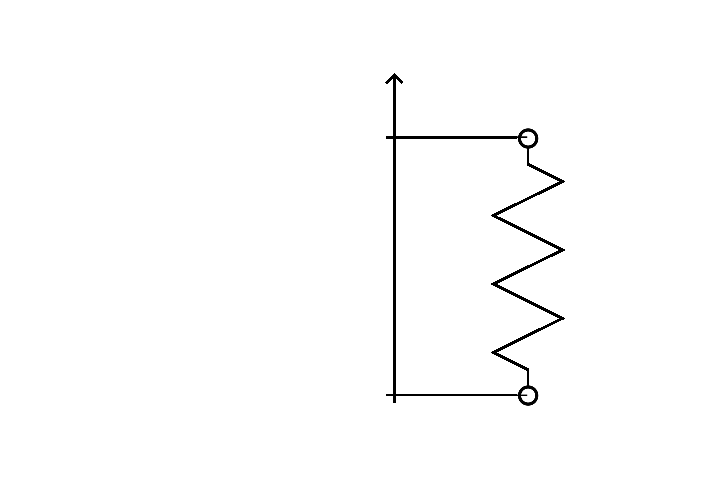
\includegraphics[width=\unitlength]{images_2ddl/repos2.eps}}%
    \put(0.53610169,0.57938811){\color[rgb]{0,0,0}\makebox(0,0)[lb]{\smash{$y$}}}%
    \put(0.29,0.46){\color[rgb]{0,0,0}\makebox(0,0)[lb]{\smash{$y_1=2R-\dfrac{m_r g}{2k}$}}}%
    \put(0.42,0.09){\color[rgb]{0,0,0}\makebox(0,0)[lb]{\smash{$y_2=0$}}}%
    \put(0.62490379,0.2696811){\color[rgb]{0,0,0}\makebox(0,0)[lb]{\smash{$k$}}}%
    \put(0.7581069,0.49168631){\color[rgb]{0,0,0}\makebox(0,0)[lb]{\smash{$\dfrac{m_r}{2}$}}}%
    \put(0.78030738,0.0698765){\color[rgb]{0,0,0}\makebox(0,0)[lb]{\smash{$\dfrac{m_r}{2}$}}}%
  \end{picture}%
\endgroup%

\caption{Système au repos. Le ressort de longueur à vide $2R$ et de raideur $k$ est écrasé par le poids de la masse supérieure.}
\label{fig:repos}
\end{figure}

\subsection{Limite en comportement linéaire}

A partir d'une certaine flèche $\delta$ imposée par une force de compression $F$, l'anneau ne se comporte plus de manière linéaire et la relation $F=k\delta$, où $k$ est la constante définie dans l'équation \ref{eq:0}, n'est plus valable. 
Afin de définir la valeur limite de $\delta$ au dessus de laquelle on sort du domaine de comportement linéaire, une étude éléments finis prenant en compte les non linéarités d'ordre géométrique est réalisée, puis comparée avec le modèle théorique linéaire. Dans cette étude, la roue est modélisée avec des éléments poutres, le déplacement $\delta$ est imposée comme paramètre d'entrée et la force $F$, relevée comme donnée de sortie, pour des raisons de convergence.
Les résultats sont présentés en figure \ref{fig:lin1}.
On considère qu'on sort de la zone de comportement linéaire lorsque la valeur absolue de l'erreur relative entre les deux modèles, $\epsilon=\frac{F_{éléments finis}-F_{théorique}}{F_{théorique}}$ dépasse les 10\%. La limite du domaine de comportement linéaire correspond donc à $\frac{delta}{R}<0.1$

\begin{figure}[h]
\centering
%% Creator: Inkscape inkscape 0.92.2, www.inkscape.org
%% PDF/EPS/PS + LaTeX output extension by Johan Engelen, 2010
%% Accompanies image file 'lineaire.eps' (pdf, eps, ps)
%%
%% To include the image in your LaTeX document, write
%%   \input{<filename>.pdf_tex}
%%  instead of
%%   \includegraphics{<filename>.pdf}
%% To scale the image, write
%%   \def\svgwidth{<desired width>}
%%   \input{<filename>.pdf_tex}
%%  instead of
%%   \includegraphics[width=<desired width>]{<filename>.pdf}
%%
%% Images with a different path to the parent latex file can
%% be accessed with the `import' package (which may need to be
%% installed) using
%%   \usepackage{import}
%% in the preamble, and then including the image with
%%   \import{<path to file>}{<filename>.pdf_tex}
%% Alternatively, one can specify
%%   \graphicspath{{<path to file>/}}
%% 
%% For more information, please see info/svg-inkscape on CTAN:
%%   http://tug.ctan.org/tex-archive/info/svg-inkscape
%%
\begingroup%
  \makeatletter%
  \providecommand\color[2][]{%
    \errmessage{(Inkscape) Color is used for the text in Inkscape, but the package 'color.sty' is not loaded}%
    \renewcommand\color[2][]{}%
  }%
  \providecommand\transparent[1]{%
    \errmessage{(Inkscape) Transparency is used (non-zero) for the text in Inkscape, but the package 'transparent.sty' is not loaded}%
    \renewcommand\transparent[1]{}%
  }%
  \providecommand\rotatebox[2]{#2}%
  \ifx\svgwidth\undefined%
    \setlength{\unitlength}{344.79999138bp}%
    \ifx\svgscale\undefined%
      \relax%
    \else%
      \setlength{\unitlength}{\unitlength * \real{\svgscale}}%
    \fi%
  \else%
    \setlength{\unitlength}{\svgwidth}%
  \fi%
  \global\let\svgwidth\undefined%
  \global\let\svgscale\undefined%
  \makeatother%
  \begin{picture}(1,0.83526682)%
    \put(0,0){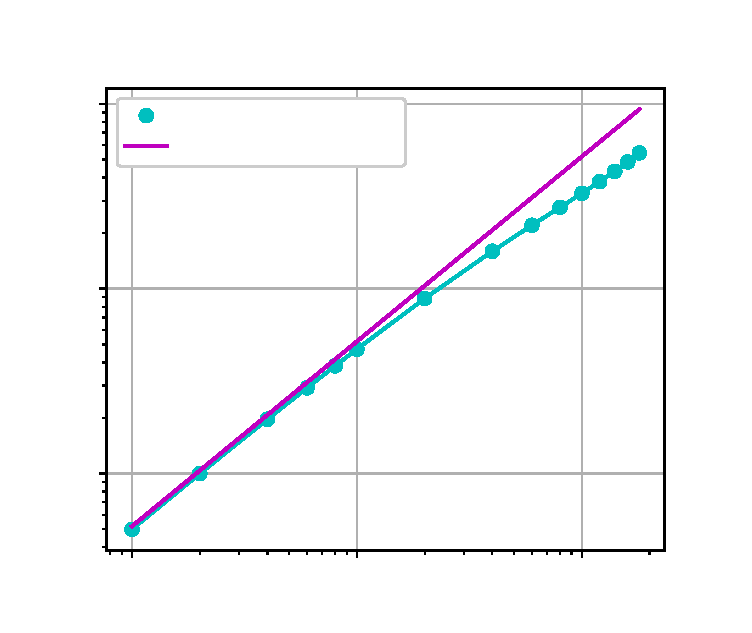
\includegraphics[width=\unitlength]{images_2ddl/lineaire.eps}}%
    \put(0.1257964,0.0485348){\color[rgb]{0,0,0}\makebox(0,0)[lb]{\smash{10}}}%
    \put(0.16297825,0.05963727){\color[rgb]{0,0,0}\makebox(0,0)[lb]{\smash{-2}}}%
    \put(0.43892111,0.04878857){\color[rgb]{0,0,0}\makebox(0,0)[lb]{\smash{10}}}%
    \put(0.47610296,0.05989104){\color[rgb]{0,0,0}\makebox(0,0)[lb]{\smash{-1}}}%
    \put(0.76074536,0.0485348){\color[rgb]{0,0,0}\makebox(0,0)[lb]{\smash{10}}}%
    \put(0.7979272,0.05963727){\color[rgb]{0,0,0}\makebox(0,0)[lb]{\smash{0}}}%
    \put(0.45736079,0.00605084){\color[rgb]{0,0,0}\makebox(0,0)[lb]{\smash{$\delta/R$ }}}%
    \put(0.05278422,0.18847651){\color[rgb]{0,0,0}\makebox(0,0)[lb]{\smash{10}}}%
    \put(0.08996607,0.19957897){\color[rgb]{0,0,0}\makebox(0,0)[lb]{\smash{2}}}%
    \put(0.05278422,0.44581787){\color[rgb]{0,0,0}\makebox(0,0)[lb]{\smash{10}}}%
    \put(0.08996607,0.45692033){\color[rgb]{0,0,0}\makebox(0,0)[lb]{\smash{3}}}%
    \put(0.05278422,0.70196636){\color[rgb]{0,0,0}\makebox(0,0)[lb]{\smash{10}}}%
    \put(0.08996607,0.71306882){\color[rgb]{0,0,0}\makebox(0,0)[lb]{\smash{4}}}%
    \put(0.03515632,0.373692){\color[rgb]{0,0,0}\rotatebox{90}{\makebox(0,0)[lb]{\smash{$F (N)$ }}}}%
    \put(0.23259861,0.68690835){\color[rgb]{0,0,0}\makebox(0,0)[lb]{\smash{étude éléments finis}}}%
    \put(0.23259861,0.64435615){\color[rgb]{0,0,0}\makebox(0,0)[lb]{\smash{théorie}}}%
  \end{picture}%
\endgroup%

\caption{Comparaison entre une étude éléments finis d'une roue réalisée avec des éléments poutres, dans laquelle on prend en compte les non linéarités géométrique, et le modèle théorique linéaire où la force appliquée et le déplacement sont liés par la constante $k$ selon la relation $F=k \delta$}
\label{fig:lin1}
\end{figure}

En dérivant la courbe de $F=f(\delta)$ obtenue par analyse éléments finis, on obtient l'évolution de la raideur $k$ en fonction de $\frac{\delta}{R}$. Le résultat est présenté en figure \ref{fig:lin2}. Dans le domaine linéaire, on prendre comme valeur de $k$ la valeur moyenne des points situés dans la zone $\frac{\delta}{R}<0.1$

\begin{figure}[h]
\centering
%% Creator: Inkscape inkscape 0.92.2, www.inkscape.org
%% PDF/EPS/PS + LaTeX output extension by Johan Engelen, 2010
%% Accompanies image file 'lineaire2.eps' (pdf, eps, ps)
%%
%% To include the image in your LaTeX document, write
%%   \input{<filename>.pdf_tex}
%%  instead of
%%   \includegraphics{<filename>.pdf}
%% To scale the image, write
%%   \def\svgwidth{<desired width>}
%%   \input{<filename>.pdf_tex}
%%  instead of
%%   \includegraphics[width=<desired width>]{<filename>.pdf}
%%
%% Images with a different path to the parent latex file can
%% be accessed with the `import' package (which may need to be
%% installed) using
%%   \usepackage{import}
%% in the preamble, and then including the image with
%%   \import{<path to file>}{<filename>.pdf_tex}
%% Alternatively, one can specify
%%   \graphicspath{{<path to file>/}}
%% 
%% For more information, please see info/svg-inkscape on CTAN:
%%   http://tug.ctan.org/tex-archive/info/svg-inkscape
%%
\begingroup%
  \makeatletter%
  \providecommand\color[2][]{%
    \errmessage{(Inkscape) Color is used for the text in Inkscape, but the package 'color.sty' is not loaded}%
    \renewcommand\color[2][]{}%
  }%
  \providecommand\transparent[1]{%
    \errmessage{(Inkscape) Transparency is used (non-zero) for the text in Inkscape, but the package 'transparent.sty' is not loaded}%
    \renewcommand\transparent[1]{}%
  }%
  \providecommand\rotatebox[2]{#2}%
  \ifx\svgwidth\undefined%
    \setlength{\unitlength}{395.9999901bp}%
    \ifx\svgscale\undefined%
      \relax%
    \else%
      \setlength{\unitlength}{\unitlength * \real{\svgscale}}%
    \fi%
  \else%
    \setlength{\unitlength}{\svgwidth}%
  \fi%
  \global\let\svgwidth\undefined%
  \global\let\svgscale\undefined%
  \makeatother%
  \begin{picture}(1,0.833939)%
    \put(0,0){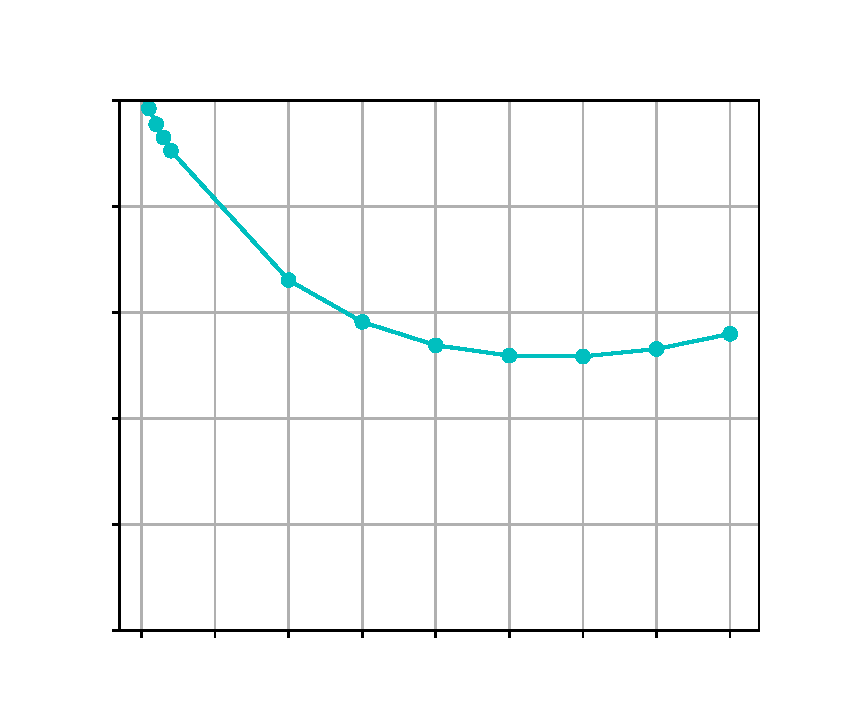
\includegraphics[width=\unitlength]{images_2ddl/lineaire2.eps}}%
    \put(0.13122525,0.05494683){\color[rgb]{0,0,0}\makebox(0,0)[lb]{\smash{0.0}}}%
    \put(0.22040808,0.05494683){\color[rgb]{0,0,0}\makebox(0,0)[lb]{\smash{0.2}}}%
    \put(0.30959091,0.05494683){\color[rgb]{0,0,0}\makebox(0,0)[lb]{\smash{0.4}}}%
    \put(0.39877273,0.05494683){\color[rgb]{0,0,0}\makebox(0,0)[lb]{\smash{0.6}}}%
    \put(0.48795707,0.05494683){\color[rgb]{0,0,0}\makebox(0,0)[lb]{\smash{0.8}}}%
    \put(0.57714141,0.05494683){\color[rgb]{0,0,0}\makebox(0,0)[lb]{\smash{1.0}}}%
    \put(0.66632323,0.05494683){\color[rgb]{0,0,0}\makebox(0,0)[lb]{\smash{1.2}}}%
    \put(0.75550505,0.05494683){\color[rgb]{0,0,0}\makebox(0,0)[lb]{\smash{1.4}}}%
    \put(0.84468939,0.05494683){\color[rgb]{0,0,0}\makebox(0,0)[lb]{\smash{1.6}}}%
    \put(0.09126414,0.08221173){\color[rgb]{0,0,0}\makebox(0,0)[lb]{\smash{0}}}%
    \put(0.04308712,0.21073142){\color[rgb]{0,0,0}\makebox(0,0)[lb]{\smash{1000}}}%
    \put(0.04308712,0.33925213){\color[rgb]{0,0,0}\makebox(0,0)[lb]{\smash{2000}}}%
    \put(0.04308712,0.46777233){\color[rgb]{0,0,0}\makebox(0,0)[lb]{\smash{3000}}}%
    \put(0.04308712,0.59629254){\color[rgb]{0,0,0}\makebox(0,0)[lb]{\smash{4000}}}%
    \put(0.04308712,0.72481274){\color[rgb]{0,0,0}\makebox(0,0)[lb]{\smash{5000}}}%
    \put(0.48795707,0.01){\color[rgb]{0,0,0}\makebox(0,0)[lb]{\smash{$\delta/R$ }}}%
    \put(0.02773838,0.36184557){\color[rgb]{0,0,0}\rotatebox{90}{\makebox(0,0)[lb]{\smash{$k$ $ (N \cdot m^{-1})$ }}}}%
  \end{picture}%
\endgroup%

\caption{Évolution du coefficient de raideur $k$ en fonction du ratio $\delta/R$. Cette courbe est obtenue par la dérivation des points obtenus par analyse éléments finis de la figure \ref{fig:lin1}, en utilisant la méthode des différences finies centrées.}
\label{fig:lin2}
\end{figure}

\subsection{Mise en équations}

On note $t=-t_0$ le moment auquel on relâche le ressort, $t=0$ le moment auquel la masse inférieure quitte le sol et $t_f$ le moment auquel le centre de gravité du système atteint sa hauteur maximale.
\\

\begin{figure}[h]

\def\svgwidth{400}
%% Creator: Inkscape inkscape 0.92.2, www.inkscape.org
%% PDF/EPS/PS + LaTeX output extension by Johan Engelen, 2010
%% Accompanies image file 'saut1.eps' (pdf, eps, ps)
%%
%% To include the image in your LaTeX document, write
%%   \input{<filename>.pdf_tex}
%%  instead of
%%   \includegraphics{<filename>.pdf}
%% To scale the image, write
%%   \def\svgwidth{<desired width>}
%%   \input{<filename>.pdf_tex}
%%  instead of
%%   \includegraphics[width=<desired width>]{<filename>.pdf}
%%
%% Images with a different path to the parent latex file can
%% be accessed with the `import' package (which may need to be
%% installed) using
%%   \usepackage{import}
%% in the preamble, and then including the image with
%%   \import{<path to file>}{<filename>.pdf_tex}
%% Alternatively, one can specify
%%   \graphicspath{{<path to file>/}}
%% 
%% For more information, please see info/svg-inkscape on CTAN:
%%   http://tug.ctan.org/tex-archive/info/svg-inkscape
%%
\begingroup%
  \makeatletter%
  \providecommand\color[2][]{%
    \errmessage{(Inkscape) Color is used for the text in Inkscape, but the package 'color.sty' is not loaded}%
    \renewcommand\color[2][]{}%
  }%
  \providecommand\transparent[1]{%
    \errmessage{(Inkscape) Transparency is used (non-zero) for the text in Inkscape, but the package 'transparent.sty' is not loaded}%
    \renewcommand\transparent[1]{}%
  }%
  \providecommand\rotatebox[2]{#2}%
  \ifx\svgwidth\undefined%
    \setlength{\unitlength}{458.93788937bp}%
    \ifx\svgscale\undefined%
      \relax%
    \else%
      \setlength{\unitlength}{\unitlength * \real{\svgscale}}%
    \fi%
  \else%
    \setlength{\unitlength}{\svgwidth}%
  \fi%
  \global\let\svgwidth\undefined%
  \global\let\svgscale\undefined%
  \makeatother%
  \begin{picture}(1,0.55996795)%
    \put(0,0){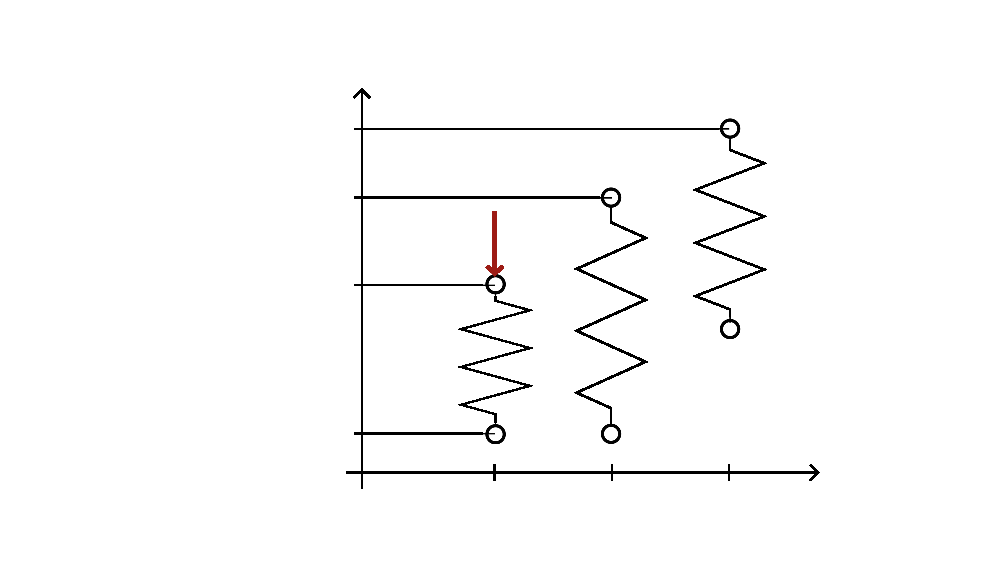
\includegraphics[width=\unitlength]{images_2ddl/saut1.eps}}%
    \put(0.35332121,0.50424636){\color[rgb]{0,0,0}\makebox(0,0)[lb]{\smash{$y$}}}%
    \put(0.85079889,0.07843695){\color[rgb]{0,0,0}\makebox(0,0)[lb]{\smash{$t$}}}%
    \put(0.44868441,0.03798154){\color[rgb]{0,0,0}\makebox(0,0)[lb]{\smash{$t<-t_0$}}}%
    \put(0.59510438,0.04003324){\color[rgb]{0,0,0}\makebox(0,0)[lb]{\smash{$t=0$}}}%
    \put(0.71660123,0.03978188){\color[rgb]{0,0,0}\makebox(0,0)[lb]{\smash{$t=t_f$}}}%
    \put(0.31206609,0.11596114){\color[rgb]{0,0,0}\makebox(0,0)[lb]{\smash{$0$}}}%
    \put(0.12576987,0.27218246){\color[rgb]{0,0,0}\makebox(0,0)[lb]{\smash{$2R-\dfrac{F}{k}-\dfrac{m_r g}{2k}$}}}%
    \put(0.19576987,0.36438468){\color[rgb]{0,0,0}\makebox(0,0)[lb]{\smash{$2R+\dfrac{m_r g}{2k}$}}}%
    \put(0.25429501,0.44056847){\color[rgb]{0,0,0}\makebox(0,0)[lb]{\smash{$y_{1,max}$}}}%
    \put(0.51238222,0.3284082){\color[rgb]{0.61568627,0.10588235,0.07843137}\makebox(0,0)[lb]{\smash{$F$}}}%
  \end{picture}%
\endgroup%


\caption{Saut du système. Pour $t<-t_0$, le système est écrasé par une force F. Il est relâche à $t=-t_0$, et la masse inférieure quitte le sol à $t=0$. Le centre de gravité du système atteint sa hauteur maximale pour $t=t_f$}
\label{fig:saut}
\end{figure}

$$
$$
$$
$$


Avant que la masse inférieure ne quitte le sol ($y_2=0$), la masse supérieure est soumise à deux forces de directions confondues avec l'axe du ressort: son propre poids de norme $-\frac{m_r g}{2}$, et la force élastique de norme $-k(y_1-2R)$. Son mouvement est régi par:

\begin{equation}
    \frac{m_r}{2}\frac{d^2y_1}{dt^2}+k(y_1-2R)+\frac{m_r}{2}g=0,
  \label{eq:1}
\end{equation}
pour $-t_0<t<0$,\\

avec les condition initiales:

\begin{align}
    &y_1(-t_0)=2R-\frac{F}{k}-\frac{m_r g}{2k} \nonumber\\
    &\frac{dy_1}{dt}(-t_0)=0
\label{eq:1i}
\end{align}


et où $g$ est l'accélération gravitationnelle. \\
  
A partir du moment où la masse inférieure quitte le sol, la force qui lui est transmise par le ressort devient suffisante pour prendre le dessus sur la gravité: $\frac{m_r g}{2}=k(y_1-2R)$  et la position des deux masses est donnée par:

\begin{align}
    \frac{m_r}{2}\frac{d^2y_1}{dt^2}+k(y_1-y_2-2R)+\frac{m_r}{2}g&=0 \nonumber\\
    \frac{m_r}{2}\frac{d^2y_2}{dt^2}+k(y_2-y_1+2R)+\frac{m_r}{2}g&=0,
  \label{eq:3}
\end{align}

pour $0<t<t_f$,\\
avec les conditions initiales: 

\begin{align}
    y_1(0)=&2R+\frac{m_r g}{2k} & \frac{d y_1}{dt}(0)=&v_{10}\nonumber\\
    y_2(0)=&0 & \frac{d y2}{dt}(0)=&0
  \label{eq:4}
\end{align}    
    


\begin{figure}[htb]
\centering
\def\svgwidth{350}
%% Creator: Inkscape inkscape 0.92.2, www.inkscape.org
%% PDF/EPS/PS + LaTeX output extension by Johan Engelen, 2010
%% Accompanies image file 'sautp.eps' (pdf, eps, ps)
%%
%% To include the image in your LaTeX document, write
%%   \input{<filename>.pdf_tex}
%%  instead of
%%   \includegraphics{<filename>.pdf}
%% To scale the image, write
%%   \def\svgwidth{<desired width>}
%%   \input{<filename>.pdf_tex}
%%  instead of
%%   \includegraphics[width=<desired width>]{<filename>.pdf}
%%
%% Images with a different path to the parent latex file can
%% be accessed with the `import' package (which may need to be
%% installed) using
%%   \usepackage{import}
%% in the preamble, and then including the image with
%%   \import{<path to file>}{<filename>.pdf_tex}
%% Alternatively, one can specify
%%   \graphicspath{{<path to file>/}}
%% 
%% For more information, please see info/svg-inkscape on CTAN:
%%   http://tug.ctan.org/tex-archive/info/svg-inkscape
%%
\begingroup%
  \makeatletter%
  \providecommand\color[2][]{%
    \errmessage{(Inkscape) Color is used for the text in Inkscape, but the package 'color.sty' is not loaded}%
    \renewcommand\color[2][]{}%
  }%
  \providecommand\transparent[1]{%
    \errmessage{(Inkscape) Transparency is used (non-zero) for the text in Inkscape, but the package 'transparent.sty' is not loaded}%
    \renewcommand\transparent[1]{}%
  }%
  \providecommand\rotatebox[2]{#2}%
  \ifx\svgwidth\undefined%
    \setlength{\unitlength}{431.9999892bp}%
    \ifx\svgscale\undefined%
      \relax%
    \else%
      \setlength{\unitlength}{\unitlength * \real{\svgscale}}%
    \fi%
  \else%
    \setlength{\unitlength}{\svgwidth}%
  \fi%
  \global\let\svgwidth\undefined%
  \global\let\svgscale\undefined%
  \makeatother%
  \begin{picture}(1,0.83333334)%
    \put(0,0){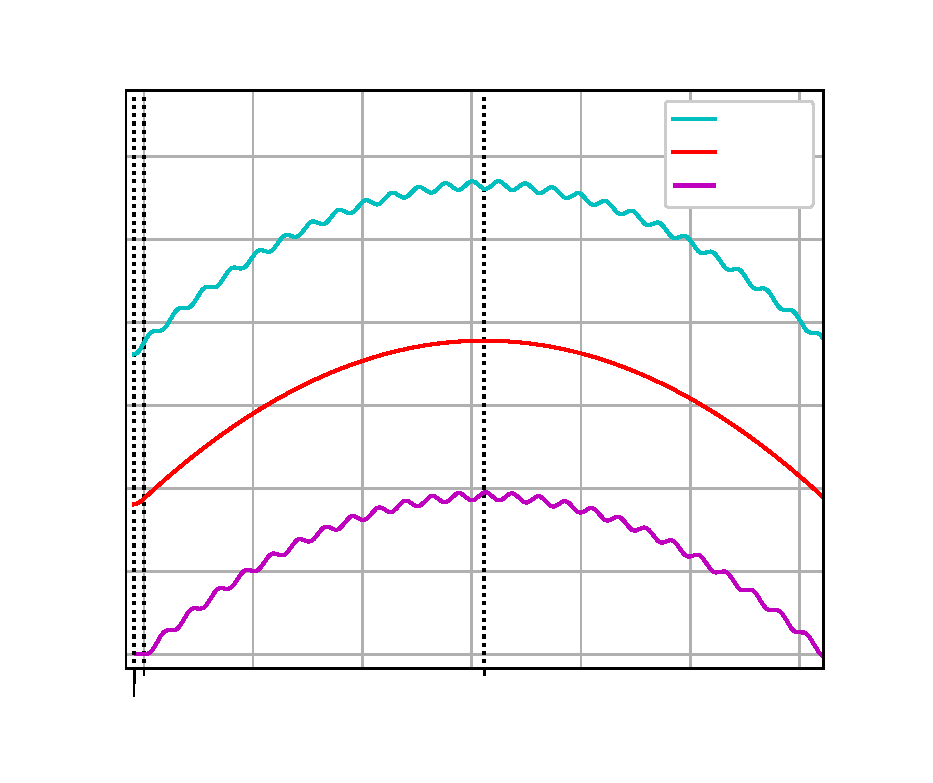
\includegraphics[width=\unitlength]{images_2ddl/sautp.eps}}%
    \put(0.79467593,0.71228239){\color[rgb]{0,0,0}\makebox(0,0)[lb]{\smash{$y_1(t)$}}}%
    \put(0.79467593,0.67524535){\color[rgb]{0,0,0}\makebox(0,0)[lb]{\smash{$y_{cdg}(t)$}}}%
    \put(0.79467593,0.63820832){\color[rgb]{0,0,0}\makebox(0,0)[lb]{\smash{$y_2(t)$}}}%
    \put(0.09341219,0.0388418){\color[rgb]{0,0,0}\makebox(0,0)[lb]{\smash{$-t_0$}}}%
    \put(0.135556003,0.06552941){\color[rgb]{0,0,0}\makebox(0,0)[lb]{\smash{$0$}}}%
    \put(0.5175824,0.06311792){\color[rgb]{0,0,0}\makebox(0,0)[lb]{\smash{$t_f$}}}%
    \put(0.05446337,0.76775099){\color[rgb]{0,0,0}\makebox(0,0)[lb]{\smash{$y (m)$}}}%
    \put(0.86146302,0.06058865){\color[rgb]{0,0,0}\makebox(0,0)[lb]{\smash{$t (s)$}}}%
  \end{picture}%
\endgroup%


\caption{Evolution temportelle des positions des masses et du centre de gravité lors du saut du système}
\label{fig:saut}
\end{figure}

Avant de résoudre le problème, on le réécrit sous forme adimensionnelle:
on définit le temps adimensionnel $\tau=t\sqrt{\frac{2k}{m_r}}$ et les variables positions adimensionnelles: $\xi_1=y_1 (\frac{2k}{m_r g})$ et $\xi_2=y_2 (\frac{2k}{m_r g})$ \\

 L'équation \ref{eq:1} devient alors:
\begin{equation}
    \frac{d^2\xi_1}{d\tau^2}+\xi_1-\xi_0+1=0,
  \label{eq:1a}
\end{equation}
\\
avec $\xi_0=\frac{4Rk}{m_r g}$,

pour $-\tau_0<\tau<0$, $\tau_0=t_0 \sqrt{\frac{2k}{m_r}}$\\

et avec les conditions initiales
\begin{align}
    &\xi_1(-\tau_0)=\xi_0-\frac{2F}{m_r g}-1 \nonumber\\
    &\frac{d\xi_1}{d\tau}(-\tau_0)=0
\label{eq:1ia}
\end{align}
 

et \ref{eq:3} devient:

\begin{align}
    \frac{d^2\xi_1}{d\tau^2}+\xi_1-\xi_2-\xi_0+1&=0 \nonumber\\
    \frac{d^2\xi_2}{d\tau^2}+\xi_2-\xi_1+\xi_0+1&=0
  \label{eq:3a}
\end{align}

pour $0<\tau<\tau_f$, $\tau_f=t_f \sqrt{\frac{2k}{m_r}}$ \\
avec les conditions initiales: 
\begin{align}
    \xi_1(0)&=\xi_0+1   &  \frac{d xi_1}{d\tau}(0)&=\zeta_{10} \nonumber\\
    \xi_2(0)&=0   &  \frac{d \xi_2}{d\tau}(0)&=0
  \label{eq:4a}
\end{align} 

En résolvant \ref{eq:1a} avec les conditions initiales \ref{eq:1ia}, on obtient l'équation du mouvement \ref{eq:2} pour $-\tau_0<\tau<0$:

\begin{align}
    \xi_1&=-frac{-2F}{m_r g}(\cos{-\tau_0}\cos{\tau}+\sin{-\tau_0}\sin{\tau})+\xi_0-1 \nonumber\\
    \xi_2&=0
  \label{eq:2}
\end{align}

En résolvant \ref{eq:3a} avec les conditions initiales \ref{eq:4a}, on obtient l'équation du mouvement \ref{eq:5a} pour $0<\tau<\tau_f$:

\begin{align}
    \xi_1&=-\frac{1}{2}\tau^2+\frac{\zeta_{10}}{2}\tau+\frac{\zeta_{10}}{2\sqrt{2}}\sin{(\sqrt{2}\tau)}+\frac{1}{2}\cos{(\sqrt{2}\tau)}+\xi_0+\frac{1}{2} \nonumber\\
    \xi_2&=-\frac{1}{2}\tau^2+\frac{\zeta_{10}}{2}\tau-\frac{\zeta_{10}}{2\sqrt{2}}\sin{(\sqrt{2}\tau)}-\frac{1}{2}\cos{(\sqrt{2}\tau)}-\frac{1}{2}
  \label{eq:5a}
\end{align}

La vitesse initiale adimensionnelle de la masse supérieure s'exprime
\begin{equation}
    \zeta_{10}=\frac{d\xi_1}{d\tau}(0)=-\frac{2F}{m_r g}\sin{-\tau_0}
    \label{eq:c1}
\end{equation}


D'après les conditions initiales \ref{eq:4a} appliquées à l'équation \ref{eq:2}, on a par continuité:
\begin{equation}
    \cos{-\tau_0}=-\frac{m_r g}{F}
    \label{eq:c2}
\end{equation}

On substitue \ref{eq:c2} à l'intérieur de \ref{eq:c1}, ce qui donne:
\begin{equation}
    \zeta_{10}=\sqrt{(\frac{2F}{m_r g})^2-4}
    \label{eq:c3}
\end{equation}

La positon adimensionnelle du centre de gravité du système s'écrit $\xi_{cdg}(\tau)=\dfrac{\xi_1(\tau)+\xi_2(\tau)}{2}$. En substituant \ref{eq:5a} dans cette expression, on obtient: 

\begin{equation}
  \xi_{cdg}(\tau)=-\frac{1}{2}\tau^2+\frac{\zeta_{10}}{2}\tau+\frac{\xi_0+1}{2}
  \label{eq:cdg}
\end{equation}

En substituant \ref{eq:c3} dans \ref{eq:cdg} on obtient:

\begin{equation}
  \xi_{cdg}(\tau)=-\frac{1}{2}\tau^2+\sqrt{(\frac{F}{m_r g})^2-1}\tau+\frac{\xi_0+1}{2}
  \label{eq:cdg2}
\end{equation}



Ces équations permettent de tracer des animations du mouvement afin de mieux appréhender ce dernier par la suite. Tout au long de l'élévation du centre de gravité de la roue, on peut observer des déformations correspondant au second mode vibratoire d'un anneau (déformations planes).
\\ 
\\


Lorsqu'on arrive à $\tau=\tau_f$, la vitesse du centre de gravité s'annule. En dérivant \ref{eq:cdg2}, on trouve l'expression de $\tau_f$:

\begin{equation}
    \tau_f=\sqrt{(\frac{F}{m_r g})^2-1}
    \label{eq:tauf}
\end{equation}

On substitue ensuite \ref{eq:tauf} à l'intérieur de \ref{eq:cdg2} pour obtenir l'expression de la hauteur maximale du centre de gravité:

\begin{equation}
  \xi_{cdg,max}=\frac{1}{2}((\frac{F}{m_r g})^2-1)+\frac{\xi_0+1}{2}
  \label{eq:cdgmax}
\end{equation}

On soustrait ensuite à \ref{eq:cdgmax} sa position adimensionnelle à l'équilibre statique $\xi_{cdg,ref}=\dfrac{\xi_0-1}{2}$ pour obtenir l'expression adimensionnelle $\eta_{max}=\dfrac{2k}{m_rg}H_{max}$:


\begin{equation}
\eta_{max}=\frac{1}{2}((\frac{F}{m_r g})^2+1)
 \label{eq:hmax}
\end{equation}


Ainsi, les paramètres influençant la hauteur maximale de saut du système sont:
\begin{itemize}
    \item La force de compression $F$ à laquelle ce dernier est soumis initialement
    \item La masse du système, déterminée par sa géométrie et la masse volumique du matériau
    \item La raideur équivalente du système qui dépend de sa géométrie et du module de Young du matériau.
\end{itemize}

L'expression de $H_{max}$ nous permet d'étudier l'efficacité énergétique du système, c'est à dire d'estimer quelle fraction de l'énergie totale fournie au système sous forme de déformation élastique est convertie en énergie potentielle gravitationnelle servant au saut. \\
Pour cela on s'intéresse au ratio $\frac{E_{p,g}}{E_{tot}}$ de ces deux quantités. \\
Avec $E_{tot}=\dfrac{F^2}{2k}$ et $E_{p,g}=m_r g H_{max}$, on obtient:  $\dfrac{E_{p,g}}{E_{tot}}=\dfrac{1}{2}((\dfrac{m_r g}{F})^2+1)$.

\subsection{Traitement numérique du modèle}
Dans la partie qui suit, on étudie les variations de $\eta_{max}$, la hauteur maximle de saut adimensionnelle et du ratio d'efficacité énergétique.
\\ 
\\ 
Les paramètres $F$, $k$ et $m_r$ doivent rester supérieurs aux valeurs limites suivantes, en dessous desquelles le modèle n'est plus valide:
\begin{itemize}
    \item Pour $F$: Pour que le modèle soit valide il faut qu’il y ait un saut, l'énergie de déformation élastique doit être suffisante pour faire décoller le système, ce qui se traduit par: $\dfrac{F}{m_r g}>1$
    \item Pour $k$: Le ressort doit pouvoir soutenir la masse 1: $\frac{m_r g}{2k}<2R$ c'est à dire: $k>\frac{m_r g}{4R}$ 
    \item Pour $m_r$: Diminuer $m_r$ revient à retirer de la matière, il y a donc une masse limite dépendant des propriétés mécaniques du matériau en dessous de laquelle il y aura rupture lors de la compression, la roue étant devenue trop fragile. Ce point là sera développé au chapitre \ref{sec:Theme3}.
\end{itemize}
Les limites seront indiquées par des pointillés sur les tracés des figures \ref{fig:eta} et \ref{fig:effe}.
\\

\begin{figure}[htb]
\centering
\def\svgwidth{320}
%% Creator: Inkscape inkscape 0.92.2, www.inkscape.org
%% PDF/EPS/PS + LaTeX output extension by Johan Engelen, 2010
%% Accompanies image file 'eta.eps' (pdf, eps, ps)
%%
%% To include the image in your LaTeX document, write
%%   \input{<filename>.pdf_tex}
%%  instead of
%%   \includegraphics{<filename>.pdf}
%% To scale the image, write
%%   \def\svgwidth{<desired width>}
%%   \input{<filename>.pdf_tex}
%%  instead of
%%   \includegraphics[width=<desired width>]{<filename>.pdf}
%%
%% Images with a different path to the parent latex file can
%% be accessed with the `import' package (which may need to be
%% installed) using
%%   \usepackage{import}
%% in the preamble, and then including the image with
%%   \import{<path to file>}{<filename>.pdf_tex}
%% Alternatively, one can specify
%%   \graphicspath{{<path to file>/}}
%% 
%% For more information, please see info/svg-inkscape on CTAN:
%%   http://tug.ctan.org/tex-archive/info/svg-inkscape
%%
\begingroup%
  \makeatletter%
  \providecommand\color[2][]{%
    \errmessage{(Inkscape) Color is used for the text in Inkscape, but the package 'color.sty' is not loaded}%
    \renewcommand\color[2][]{}%
  }%
  \providecommand\transparent[1]{%
    \errmessage{(Inkscape) Transparency is used (non-zero) for the text in Inkscape, but the package 'transparent.sty' is not loaded}%
    \renewcommand\transparent[1]{}%
  }%
  \providecommand\rotatebox[2]{#2}%
  \ifx\svgwidth\undefined%
    \setlength{\unitlength}{344.79999138bp}%
    \ifx\svgscale\undefined%
      \relax%
    \else%
      \setlength{\unitlength}{\unitlength * \real{\svgscale}}%
    \fi%
  \else%
    \setlength{\unitlength}{\svgwidth}%
  \fi%
  \global\let\svgwidth\undefined%
  \global\let\svgscale\undefined%
  \makeatother%
  \begin{picture}(1,0.83526682)%
    \put(0,0){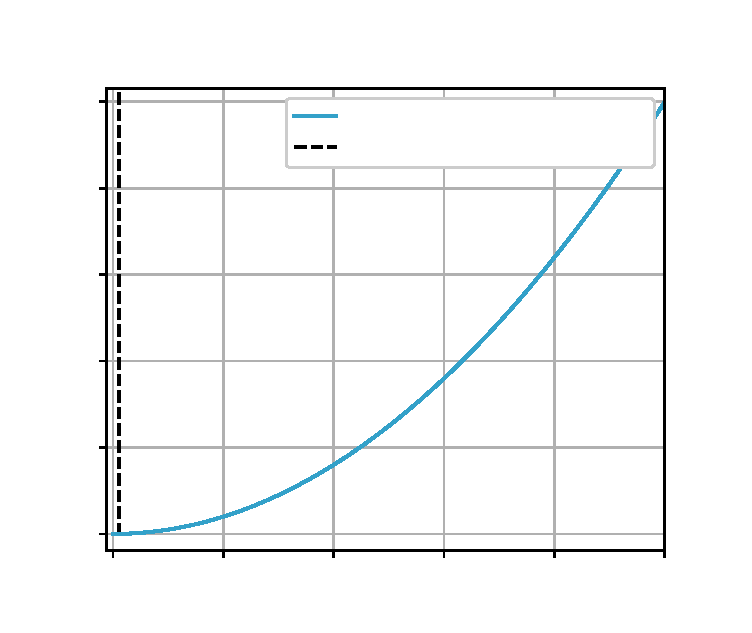
\includegraphics[width=\unitlength]{images_2ddl/eta.eps}}%
    \put(0.12494664,0.04955423){\color[rgb]{0,0,0}\makebox(0,0)[lb]{\smash{0}}}%
    \put(0.26935006,0.04955423){\color[rgb]{0,0,0}\makebox(0,0)[lb]{\smash{20}}}%
    \put(0.42297564,0.04955423){\color[rgb]{0,0,0}\makebox(0,0)[lb]{\smash{40}}}%
    \put(0.57660093,0.04955423){\color[rgb]{0,0,0}\makebox(0,0)[lb]{\smash{60}}}%
    \put(0.73022622,0.04955423){\color[rgb]{0,0,0}\makebox(0,0)[lb]{\smash{80}}}%
    \put(0.87462877,0.04955423){\color[rgb]{0,0,0}\makebox(0,0)[lb]{\smash{100}}}%
    \put(0.08654466,0.10358121){\color[rgb]{0,0,0}\makebox(0,0)[lb]{\smash{0}}}%
    \put(0.03121375,0.22391821){\color[rgb]{0,0,0}\makebox(0,0)[lb]{\smash{1000}}}%
    \put(0.03121375,0.34425464){\color[rgb]{0,0,0}\makebox(0,0)[lb]{\smash{2000}}}%
    \put(0.03121375,0.46459107){\color[rgb]{0,0,0}\makebox(0,0)[lb]{\smash{3000}}}%
    \put(0.03121375,0.58492749){\color[rgb]{0,0,0}\makebox(0,0)[lb]{\smash{4000}}}%
    \put(0.03121375,0.70526392){\color[rgb]{0,0,0}\makebox(0,0)[lb]{\smash{5000}}}%
    \put(0.46800464,0.68690835){\color[rgb]{0,0,0}\makebox(0,0)[lb]{\smash{$\eta_{max}$}}}%
    \put(0.46800464,0.64354118){\color[rgb]{0,0,0}\makebox(0,0)[lb]{\smash{\small valeur minimale de  $F/m_r g$ }}}%
    \put(0.46,0.0155423){\color[rgb]{0,0,0}\makebox(0,0)[lb]{\smash{$F/m_r g$}}}%
  \end{picture}%
\endgroup%

\caption{Variation de la hauteur maximale de saut adimensionnelle en fonction du ratio $F/m_r g$}
\label{fig:eta}
\end{figure}


\begin{figure}[htb]
\centering
\def\svgwidth{320}
%% Creator: Inkscape inkscape 0.92.2, www.inkscape.org
%% PDF/EPS/PS + LaTeX output extension by Johan Engelen, 2010
%% Accompanies image file 'eff.eps' (pdf, eps, ps)
%%
%% To include the image in your LaTeX document, write
%%   \input{<filename>.pdf_tex}
%%  instead of
%%   \includegraphics{<filename>.pdf}
%% To scale the image, write
%%   \def\svgwidth{<desired width>}
%%   \input{<filename>.pdf_tex}
%%  instead of
%%   \includegraphics[width=<desired width>]{<filename>.pdf}
%%
%% Images with a different path to the parent latex file can
%% be accessed with the `import' package (which may need to be
%% installed) using
%%   \usepackage{import}
%% in the preamble, and then including the image with
%%   \import{<path to file>}{<filename>.pdf_tex}
%% Alternatively, one can specify
%%   \graphicspath{{<path to file>/}}
%% 
%% For more information, please see info/svg-inkscape on CTAN:
%%   http://tug.ctan.org/tex-archive/info/svg-inkscape
%%
\begingroup%
  \makeatletter%
  \providecommand\color[2][]{%
    \errmessage{(Inkscape) Color is used for the text in Inkscape, but the package 'color.sty' is not loaded}%
    \renewcommand\color[2][]{}%
  }%
  \providecommand\transparent[1]{%
    \errmessage{(Inkscape) Transparency is used (non-zero) for the text in Inkscape, but the package 'transparent.sty' is not loaded}%
    \renewcommand\transparent[1]{}%
  }%
  \providecommand\rotatebox[2]{#2}%
  \ifx\svgwidth\undefined%
    \setlength{\unitlength}{344.79999138bp}%
    \ifx\svgscale\undefined%
      \relax%
    \else%
      \setlength{\unitlength}{\unitlength * \real{\svgscale}}%
    \fi%
  \else%
    \setlength{\unitlength}{\svgwidth}%
  \fi%
  \global\let\svgwidth\undefined%
  \global\let\svgscale\undefined%
  \makeatother%
  \begin{picture}(1,0.83526682)%
    \put(0,0){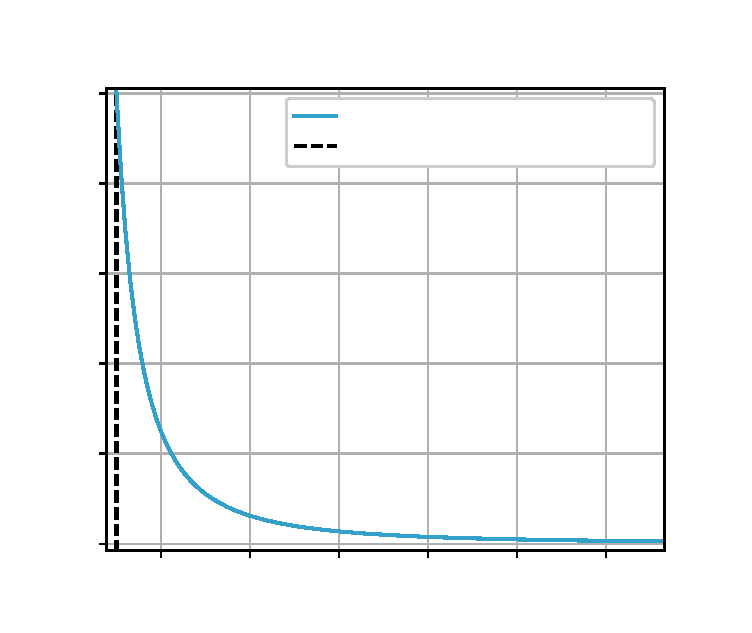
\includegraphics[width=\unitlength]{images_2ddl/eff.eps}}%
    \put(0.19169287,0.04955423){\color[rgb]{0,0,0}\makebox(0,0)[lb]{\smash{2}}}%
    \put(0.31560035,0.04955423){\color[rgb]{0,0,0}\makebox(0,0)[lb]{\smash{4}}}%
    \put(0.43950406,0.04955423){\color[rgb]{0,0,0}\makebox(0,0)[lb]{\smash{6}}}%
    \put(0.56341067,0.04955423){\color[rgb]{0,0,0}\makebox(0,0)[lb]{\smash{8}}}%
    \put(0.67809745,0.04955423){\color[rgb]{0,0,0}\makebox(0,0)[lb]{\smash{10}}}%
    \put(0.80200116,0.04955423){\color[rgb]{0,0,0}\makebox(0,0)[lb]{\smash{12}}}%
    \put(0.05885673,0.08975435){\color[rgb]{0,0,0}\makebox(0,0)[lb]{\smash{0.5}}}%
    \put(0.05885673,0.21525174){\color[rgb]{0,0,0}\makebox(0,0)[lb]{\smash{0.6}}}%
    \put(0.05885673,0.34074826){\color[rgb]{0,0,0}\makebox(0,0)[lb]{\smash{0.7}}}%
    \put(0.05885673,0.4662471){\color[rgb]{0,0,0}\makebox(0,0)[lb]{\smash{0.8}}}%
    \put(0.05885673,0.59174304){\color[rgb]{0,0,0}\makebox(0,0)[lb]{\smash{0.9}}}%
    \put(0.05885673,0.71724188){\color[rgb]{0,0,0}\makebox(0,0)[lb]{\smash{1.0}}}%
    \put(0.46800464,0.68690835){\color[rgb]{0,0,0}\makebox(0,0)[lb]{\smash{$E_{p,g}/E_{tot}$}}}%
    \put(0.46800464,0.64435615){\color[rgb]{0,0,0}\makebox(0,0)[lb]{\smash{\small valeur minimale de $F/m_r g$ }}}%
    \put(0.460200116,0.0155423){\color[rgb]{0,0,0}\makebox(0,0)[lb]{\smash{$F/m_r g$}}}%
  \end{picture}%
\endgroup%

\caption{Variation de l'efficacité énergétique en fonction du ratio $\dfrac{F}{m_r g}$}
\label{fig:effe}
\end{figure}


Remarques:
\begin{itemize}
    \item Les tracés adimensionnels permettent d'étudier une tendance globale, en s'affranchissant de la dépendance des résultats avec les autres paramètres.
    
\end{itemize}


\subsection{Comparaison avec les points de l'article \textit{Jumping hoops}}
Dans leur article \textit{Jumping hoops} \cite{yangkim}, présenté au chapitre \ref{sec:RevLitt}, Yang et Kim étudient le saut d'anneaux comprimés puis relâchés, dont le mouvement est identique à celui étudié au moyen du modèle deux degrés de liberté développé dans les sections précédentes.
Leur modèle théorique est basé sur des bilans énergétiques réalisés au moment où l'anneau quitte le sol et au moment où son centre de gravité atteint sa hauteur maximale, puis complété par leurs résultats expérimentaux, présentés par la figure \ref{fig:ykres}

\begin{figure}[htb]
\centering
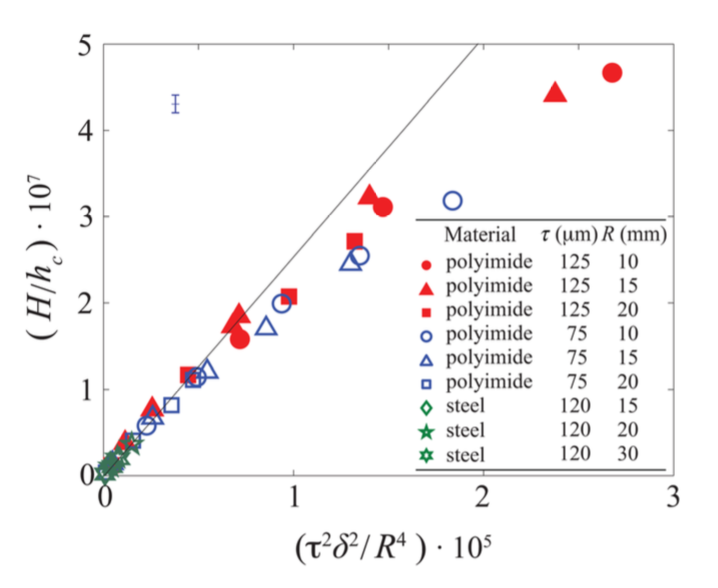
\includegraphics[width=4.5in]{images_2ddl/ykres.png}
\caption{Résultats expérimentaux de Yang et Kim, sous forme de graphique adimensionnel. $H_{max}$ représente la hauteur maximale du saut, $h_c=\frac{E}{\rho g}$, où $E$ est le module d'Young, $\rho$ la masse volumique et $g$ l'accélération gravitationnelle. $\tau$ représente la longueur d'une des côtés de la section (l'autre, $w$ est fixé à 3 mm), $R$ est le rayon médian de la roue et $\delta$ est la flèche initiale imposée.}
\label{fig:ykres}
\end{figure}

A partir de leur modèle théorique et de leurs résultats expérimentaux, Yang et Kim arrivent à la conclusion suivante: si on néglige l'énergie dissipée par la traînée, le ratio de l'énergie potentielle gravitationnelle et de l'énergie totale fournie initialement par déformation élastique est constant: $\dfrac{E_{p,g}}{E_{tot}}=0.57$.

La superposition des résultats expérimentaux de Yang et Kim et des courbes issues de nos modèles théoriques sont présentés figures \ref{fig:ykmae} et \ref{fig:yke}.
Pour ce qui concerne $H_{max}$, la figure \ref{fig:ykmae} montre que les résultats expérimentaux de Yang et Kim concordent avec le modèle théorique à deux degrés de liberté développé et étudiés dans les sections précédentes.
Pour le ratio d'efficacité énergétique $\dfrac{E_{p.g}}{E_{tot}}$, on observe des différences entre notre modèle théorique et les résultats expérimentaux de Yang et Kim.
Ces différences pourraient être expliquées d'une part par l'énergie dissipée par force de trainée que nous avons choisi de négliger dans notre modèle, et d'autre part par un comportement non linéaire du coefficient de raideur. Pour vérifier cette dernière supposition, nous calculons la valeur du ratio $\dfrac{\delta}{R}$ et la comparer à la valeur limite $0.1$ que nous avions définie au début du chapitre, au delà de laquelle on sort de la zone de comportement linéaire.

\begin{figure}[htb]
\centering
\def\svgwidth{320}
%% Creator: Inkscape inkscape 0.92.2, www.inkscape.org
%% PDF/EPS/PS + LaTeX output extension by Johan Engelen, 2010
%% Accompanies image file 'ykmae1.eps' (pdf, eps, ps)
%%
%% To include the image in your LaTeX document, write
%%   \input{<filename>.pdf_tex}
%%  instead of
%%   \includegraphics{<filename>.pdf}
%% To scale the image, write
%%   \def\svgwidth{<desired width>}
%%   \input{<filename>.pdf_tex}
%%  instead of
%%   \includegraphics[width=<desired width>]{<filename>.pdf}
%%
%% Images with a different path to the parent latex file can
%% be accessed with the `import' package (which may need to be
%% installed) using
%%   \usepackage{import}
%% in the preamble, and then including the image with
%%   \import{<path to file>}{<filename>.pdf_tex}
%% Alternatively, one can specify
%%   \graphicspath{{<path to file>/}}
%% 
%% For more information, please see info/svg-inkscape on CTAN:
%%   http://tug.ctan.org/tex-archive/info/svg-inkscape
%%
\begingroup%
  \makeatletter%
  \providecommand\color[2][]{%
    \errmessage{(Inkscape) Color is used for the text in Inkscape, but the package 'color.sty' is not loaded}%
    \renewcommand\color[2][]{}%
  }%
  \providecommand\transparent[1]{%
    \errmessage{(Inkscape) Transparency is used (non-zero) for the text in Inkscape, but the package 'transparent.sty' is not loaded}%
    \renewcommand\transparent[1]{}%
  }%
  \providecommand\rotatebox[2]{#2}%
  \ifx\svgwidth\undefined%
    \setlength{\unitlength}{395.9999901bp}%
    \ifx\svgscale\undefined%
      \relax%
    \else%
      \setlength{\unitlength}{\unitlength * \real{\svgscale}}%
    \fi%
  \else%
    \setlength{\unitlength}{\svgwidth}%
  \fi%
  \global\let\svgwidth\undefined%
  \global\let\svgscale\undefined%
  \makeatother%
  \begin{picture}(1,0.833939)%
    \put(0,0){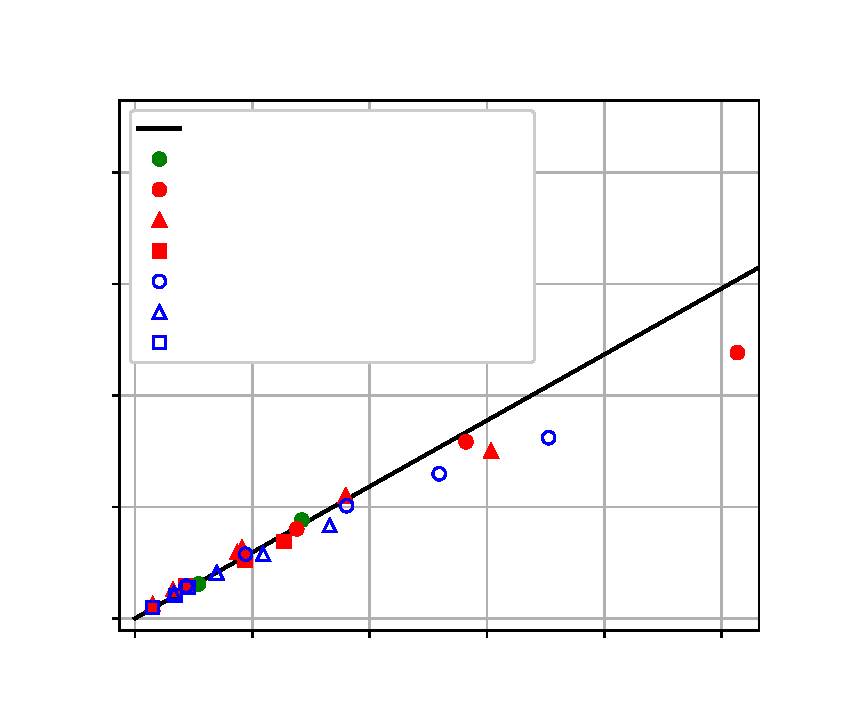
\includegraphics[width=\unitlength]{images_2ddl/ykmae1.eps}}%
    \put(0.14153535,0.05494683){\color[rgb]{0,0,0}\makebox(0,0)[lb]{\smash{0}}}%
    \put(0.26236869,0.05494683){\color[rgb]{0,0,0}\makebox(0,0)[lb]{\smash{500}}}%
    \put(0.39123232,0.05494683){\color[rgb]{0,0,0}\makebox(0,0)[lb]{\smash{1000}}}%
    \put(0.52812626,0.05494683){\color[rgb]{0,0,0}\makebox(0,0)[lb]{\smash{1500}}}%
    \put(0.6650202,0.05494683){\color[rgb]{0,0,0}\makebox(0,0)[lb]{\smash{2000}}}%
    \put(0.80191162,0.05494683){\color[rgb]{0,0,0}\makebox(0,0)[lb]{\smash{2500}}}%
    \put(0.06,0.09675819){\color[rgb]{0,0,0}\makebox(0,0)[lb]{\smash{0.0}}}%
    \put(0.06,0.23034304){\color[rgb]{0,0,0}\makebox(0,0)[lb]{\smash{5.0}}}%
    \put(0.045109697,0.365){\color[rgb]{0,0,0}\makebox(0,0)[lb]{\smash{10.0}}}%
    \put(0.045109697,0.505){\color[rgb]{0,0,0}\makebox(0,0)[lb]{\smash{15.0}}}%
    \put(0.045109697,0.645){\color[rgb]{0,0,0}\makebox(0,0)[lb]{\smash{20.0}}}%
    \put(0.025,0.33304759){\color[rgb]{0,0,0}\rotatebox{90}{\makebox(0,0)[lb]{\smash{$H_{max}/R$}}}}%
    \put(0.21843434,0.6914693){\color[rgb]{0,0,0}\makebox(0,0)[lb]{\smash{\small modèle théorique 2DDL}}}%
    \put(0.21843434,0.65442132){\color[rgb]{0,0,0}\makebox(0,0)[lb]{\smash{\small Y\&K acier (120,30)}}}%
    \put(0.21843434,0.61737082){\color[rgb]{0,0,0}\makebox(0,0)[lb]{\smash{\small Y\&K polyimide (125,10)}}}%
    \put(0.21843434,0.58032031){\color[rgb]{0,0,0}\makebox(0,0)[lb]{\smash{\small Y\&K polyimide (125,15)}}}%
    \put(0.21843434,0.54326981){\color[rgb]{0,0,0}\makebox(0,0)[lb]{\smash{\small Y\&K polyimide (125,20)}}}%
    \put(0.21843434,0.5062193){\color[rgb]{0,0,0}\makebox(0,0)[lb]{\smash{\small Y\&K polyimide (75,10)}}}%
    \put(0.21843434,0.4691688){\color[rgb]{0,0,0}\makebox(0,0)[lb]{\smash{\small Y\&K polyimide (75,15)}}}%
    \put(0.21843434,0.43211829){\color[rgb]{0,0,0}\makebox(0,0)[lb]{\smash{\small Y\&K polyimide (75,25)}}}%
    \put(0.4,0.01){\color[rgb]{0,0,0}\makebox(0,0)[lb]{\smash{ $F^2 R/(E \rho g I A)$}}}%
  \end{picture}%
\endgroup%

\caption{Graphique adimensionnel des variations de $H_{max}$ en fonction des paramètres déterminants du modèle}
\label{fig:ykmae}
\end{figure}

\begin{figure}[htb]
\centering
\def\svgwidth{320}
%% Creator: Inkscape inkscape 0.92.2, www.inkscape.org
%% PDF/EPS/PS + LaTeX output extension by Johan Engelen, 2010
%% Accompanies image file 'yke3.eps' (pdf, eps, ps)
%%
%% To include the image in your LaTeX document, write
%%   \input{<filename>.pdf_tex}
%%  instead of
%%   \includegraphics{<filename>.pdf}
%% To scale the image, write
%%   \def\svgwidth{<desired width>}
%%   \input{<filename>.pdf_tex}
%%  instead of
%%   \includegraphics[width=<desired width>]{<filename>.pdf}
%%
%% Images with a different path to the parent latex file can
%% be accessed with the `import' package (which may need to be
%% installed) using
%%   \usepackage{import}
%% in the preamble, and then including the image with
%%   \import{<path to file>}{<filename>.pdf_tex}
%% Alternatively, one can specify
%%   \graphicspath{{<path to file>/}}
%% 
%% For more information, please see info/svg-inkscape on CTAN:
%%   http://tug.ctan.org/tex-archive/info/svg-inkscape
%%
\begingroup%
  \makeatletter%
  \providecommand\color[2][]{%
    \errmessage{(Inkscape) Color is used for the text in Inkscape, but the package 'color.sty' is not loaded}%
    \renewcommand\color[2][]{}%
  }%
  \providecommand\transparent[1]{%
    \errmessage{(Inkscape) Transparency is used (non-zero) for the text in Inkscape, but the package 'transparent.sty' is not loaded}%
    \renewcommand\transparent[1]{}%
  }%
  \providecommand\rotatebox[2]{#2}%
  \ifx\svgwidth\undefined%
    \setlength{\unitlength}{690.59998274bp}%
    \ifx\svgscale\undefined%
      \relax%
    \else%
      \setlength{\unitlength}{\unitlength * \real{\svgscale}}%
    \fi%
  \else%
    \setlength{\unitlength}{\svgwidth}%
  \fi%
  \global\let\svgwidth\undefined%
  \global\let\svgscale\undefined%
  \makeatother%
  \begin{picture}(1,0.83405734)%
    \put(0,0){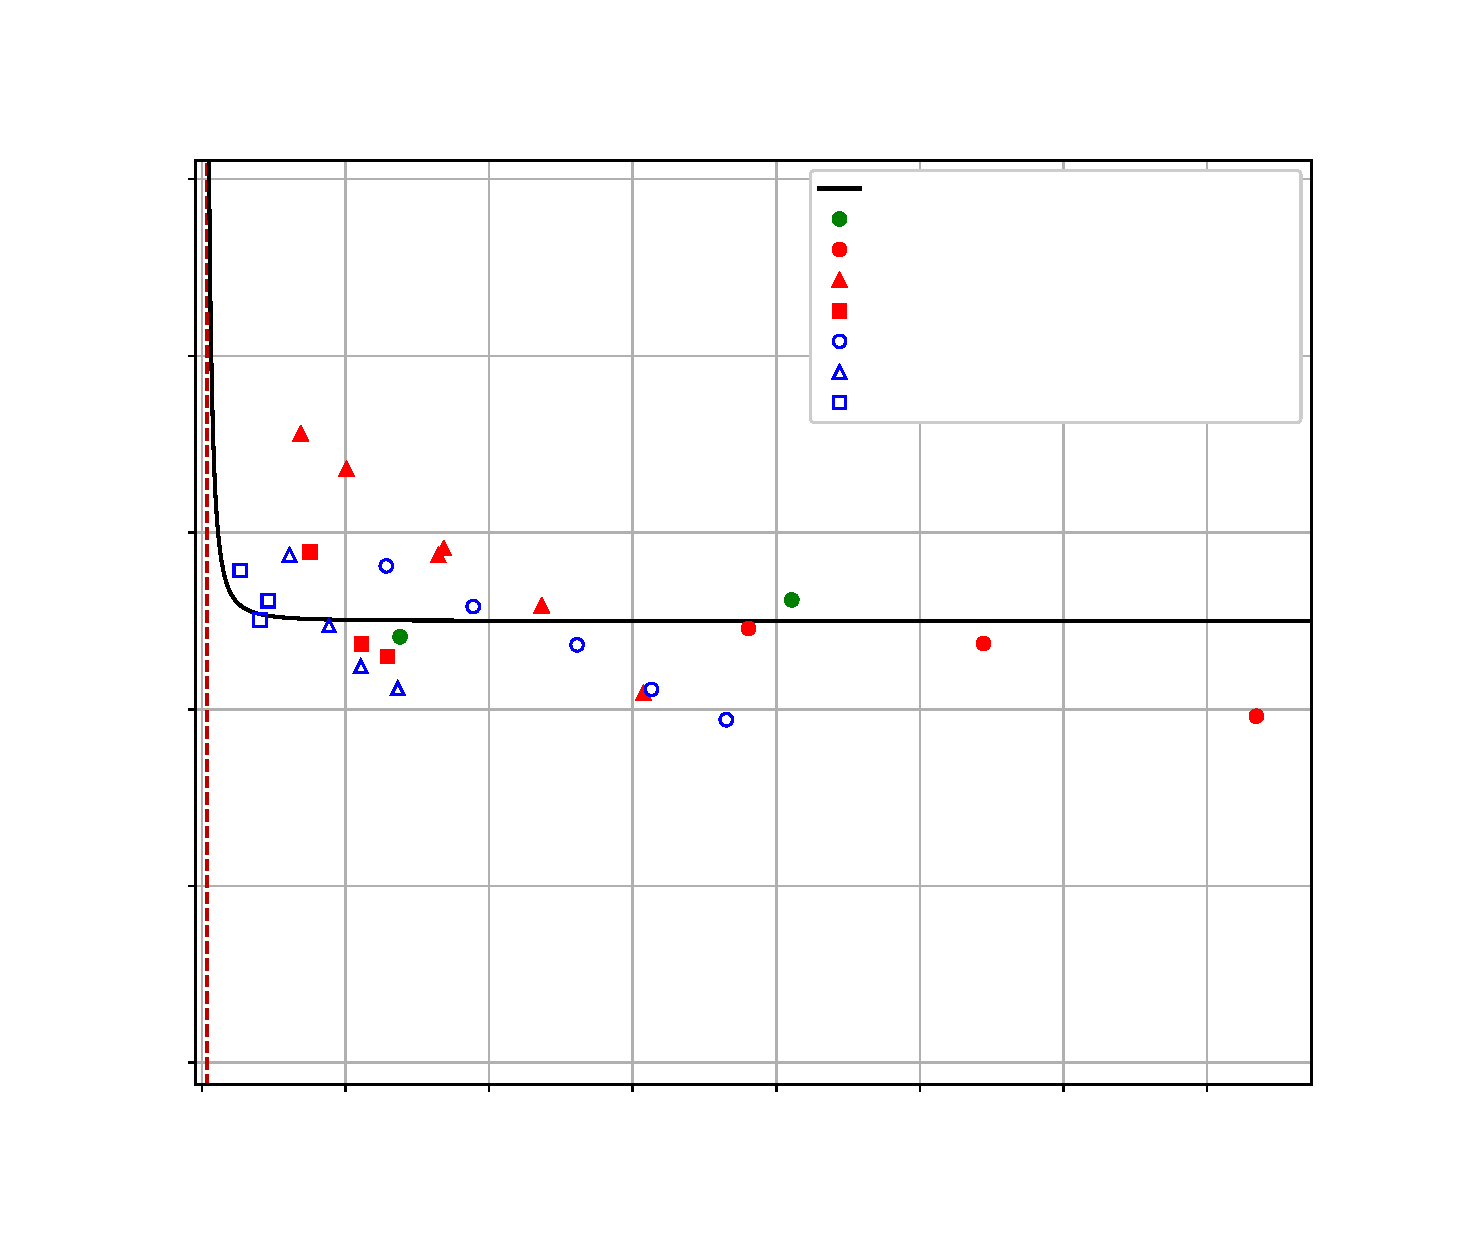
\includegraphics[width=\unitlength]{images_2ddl/yke3.eps}}%
    \put(0.11819679,0.055061454){\color[rgb]{0,0,0}\makebox(0,0)[lb]{\smash{0}}}%
    \put(0.20939183,0.055061454){\color[rgb]{0,0,0}\makebox(0,0)[lb]{\smash{20}}}%
    \put(0.30919056,0.055061454){\color[rgb]{0,0,0}\makebox(0,0)[lb]{\smash{40}}}%
    \put(0.40898928,0.055061454){\color[rgb]{0,0,0}\makebox(0,0)[lb]{\smash{60}}}%
    \put(0.50878801,0.055061454){\color[rgb]{0,0,0}\makebox(0,0)[lb]{\smash{80}}}%
    \put(0.60398349,0.055061454){\color[rgb]{0,0,0}\makebox(0,0)[lb]{\smash{100}}}%
    \put(0.70378222,0.055061454){\color[rgb]{0,0,0}\makebox(0,0)[lb]{\smash{120}}}%
    \put(0.80358094,0.055061454){\color[rgb]{0,0,0}\makebox(0,0)[lb]{\smash{140}}}%
    \put(0.067107124,0.095120895){\color[rgb]{0,0,0}\makebox(0,0)[lb]{\smash{0.0}}}%
    \put(0.067107124,0.2140501){\color[rgb]{0,0,0}\makebox(0,0)[lb]{\smash{0.2}}}%
    \put(0.067107124,0.33689111){\color[rgb]{0,0,0}\makebox(0,0)[lb]{\smash{0.4}}}%
    \put(0.067107124,0.45973212){\color[rgb]{0,0,0}\makebox(0,0)[lb]{\smash{0.6}}}%
    \put(0.067107124,0.58257457){\color[rgb]{0,0,0}\makebox(0,0)[lb]{\smash{0.8}}}%
    \put(0.067107124,0.70541558){\color[rgb]{0,0,0}\makebox(0,0)[lb]{\smash{1.0}}}%
    \put(0.04226991,0.37966696){\color[rgb]{0,0,0}\rotatebox{90}{\makebox(0,0)[lb]{\smash{$E_{p,g}/E_{tot}$}}}}%
    \put(0.59802491,0.70735418){\color[rgb]{0,0,0}\makebox(0,0)[lb]{\smash{\scriptsize modèle théorique 2DDL}}}%
    \put(0.59802491,0.68610889){\color[rgb]{0,0,0}\makebox(0,0)[lb]{\smash{\scriptsize Y\&K acier (120,30)}}}%
    \put(0.59802491,0.6648636){\color[rgb]{0,0,0}\makebox(0,0)[lb]{\smash{\scriptsize Y\&K polyimide (125,10)}}}%
    \put(0.59802491,0.6436183){\color[rgb]{0,0,0}\makebox(0,0)[lb]{\smash{\scriptsize Y\&K polyimide (125,15)}}}%
    \put(0.59802491,0.62237446){\color[rgb]{0,0,0}\makebox(0,0)[lb]{\smash{\scriptsize Y\&K polyimide (125,20)}}}%
    \put(0.59802491,0.60112916){\color[rgb]{0,0,0}\makebox(0,0)[lb]{\smash{\scriptsize Y\&K polyimide (75,10)}}}%
    \put(0.59802491,0.57988387){\color[rgb]{0,0,0}\makebox(0,0)[lb]{\smash{\scriptsize Y\&K polyimide (75,15)}}}%
    \put(0.59802491,0.55863858){\color[rgb]{0,0,0}\makebox(0,0)[lb]{\smash{\scriptsize Y\&K polyimide (75,25)}}}%
    \put(0.47,0.01){\color[rgb]{0,0,0}\makebox(0,0)[lb]{\smash{$F/m_r g$ }}}%
  \end{picture}%
\endgroup%

\caption{Variation de l'efficacité énergétique en fonction du ratio $F/(m_r g)$. La ligne pointillée rouge représente la valeur minimale que doit avoir $F$ pour qu'il y ait un saut.}
\label{fig:yke}
\end{figure}

Pour tous les points expérimentaux de Yang et Kim $\dfrac{\delta}{R}>0.1$. Pour pouvoir observer une tendance, nous élargissons le seuil de tolérance: nous traçons uniquement les points dont le ratio correspondant $\dfrac{\delta}{R}$ est inférieur à $0.35$. Le résultat, réprésenté en figure \ref{fig:ytol}, met en évidence le fait que plus on va loin au delà du domaine de comportement linéaire, plus les points expérimentaux s'éloignent de la courbe représentant notre modèle théorique. Lorsqu'on sélectionne uniquement les points de non linéarité relativement faible ($\dfrac{\delta}{R}<0.35$), ces derniers sont proches de la courbe.
Les résultats expérimentaux concordent donc avec notre modèle théorique à deux degrés de liberté développé dans les sections précédentes, qui est validé.

\begin{figure}[htb]
\centering
\def\svgwidth{320}
%% Creator: Inkscape inkscape 0.92.2, www.inkscape.org
%% PDF/EPS/PS + LaTeX output extension by Johan Engelen, 2010
%% Accompanies image file 'yktol3eps.eps' (pdf, eps, ps)
%%
%% To include the image in your LaTeX document, write
%%   \input{<filename>.pdf_tex}
%%  instead of
%%   \includegraphics{<filename>.pdf}
%% To scale the image, write
%%   \def\svgwidth{<desired width>}
%%   \input{<filename>.pdf_tex}
%%  instead of
%%   \includegraphics[width=<desired width>]{<filename>.pdf}
%%
%% Images with a different path to the parent latex file can
%% be accessed with the `import' package (which may need to be
%% installed) using
%%   \usepackage{import}
%% in the preamble, and then including the image with
%%   \import{<path to file>}{<filename>.pdf_tex}
%% Alternatively, one can specify
%%   \graphicspath{{<path to file>/}}
%% 
%% For more information, please see info/svg-inkscape on CTAN:
%%   http://tug.ctan.org/tex-archive/info/svg-inkscape
%%
\begingroup%
  \makeatletter%
  \providecommand\color[2][]{%
    \errmessage{(Inkscape) Color is used for the text in Inkscape, but the package 'color.sty' is not loaded}%
    \renewcommand\color[2][]{}%
  }%
  \providecommand\transparent[1]{%
    \errmessage{(Inkscape) Transparency is used (non-zero) for the text in Inkscape, but the package 'transparent.sty' is not loaded}%
    \renewcommand\transparent[1]{}%
  }%
  \providecommand\rotatebox[2]{#2}%
  \ifx\svgwidth\undefined%
    \setlength{\unitlength}{690.59998274bp}%
    \ifx\svgscale\undefined%
      \relax%
    \else%
      \setlength{\unitlength}{\unitlength * \real{\svgscale}}%
    \fi%
  \else%
    \setlength{\unitlength}{\svgwidth}%
  \fi%
  \global\let\svgwidth\undefined%
  \global\let\svgscale\undefined%
  \makeatother%
  \begin{picture}(1,0.83405734)%
    \put(0,0){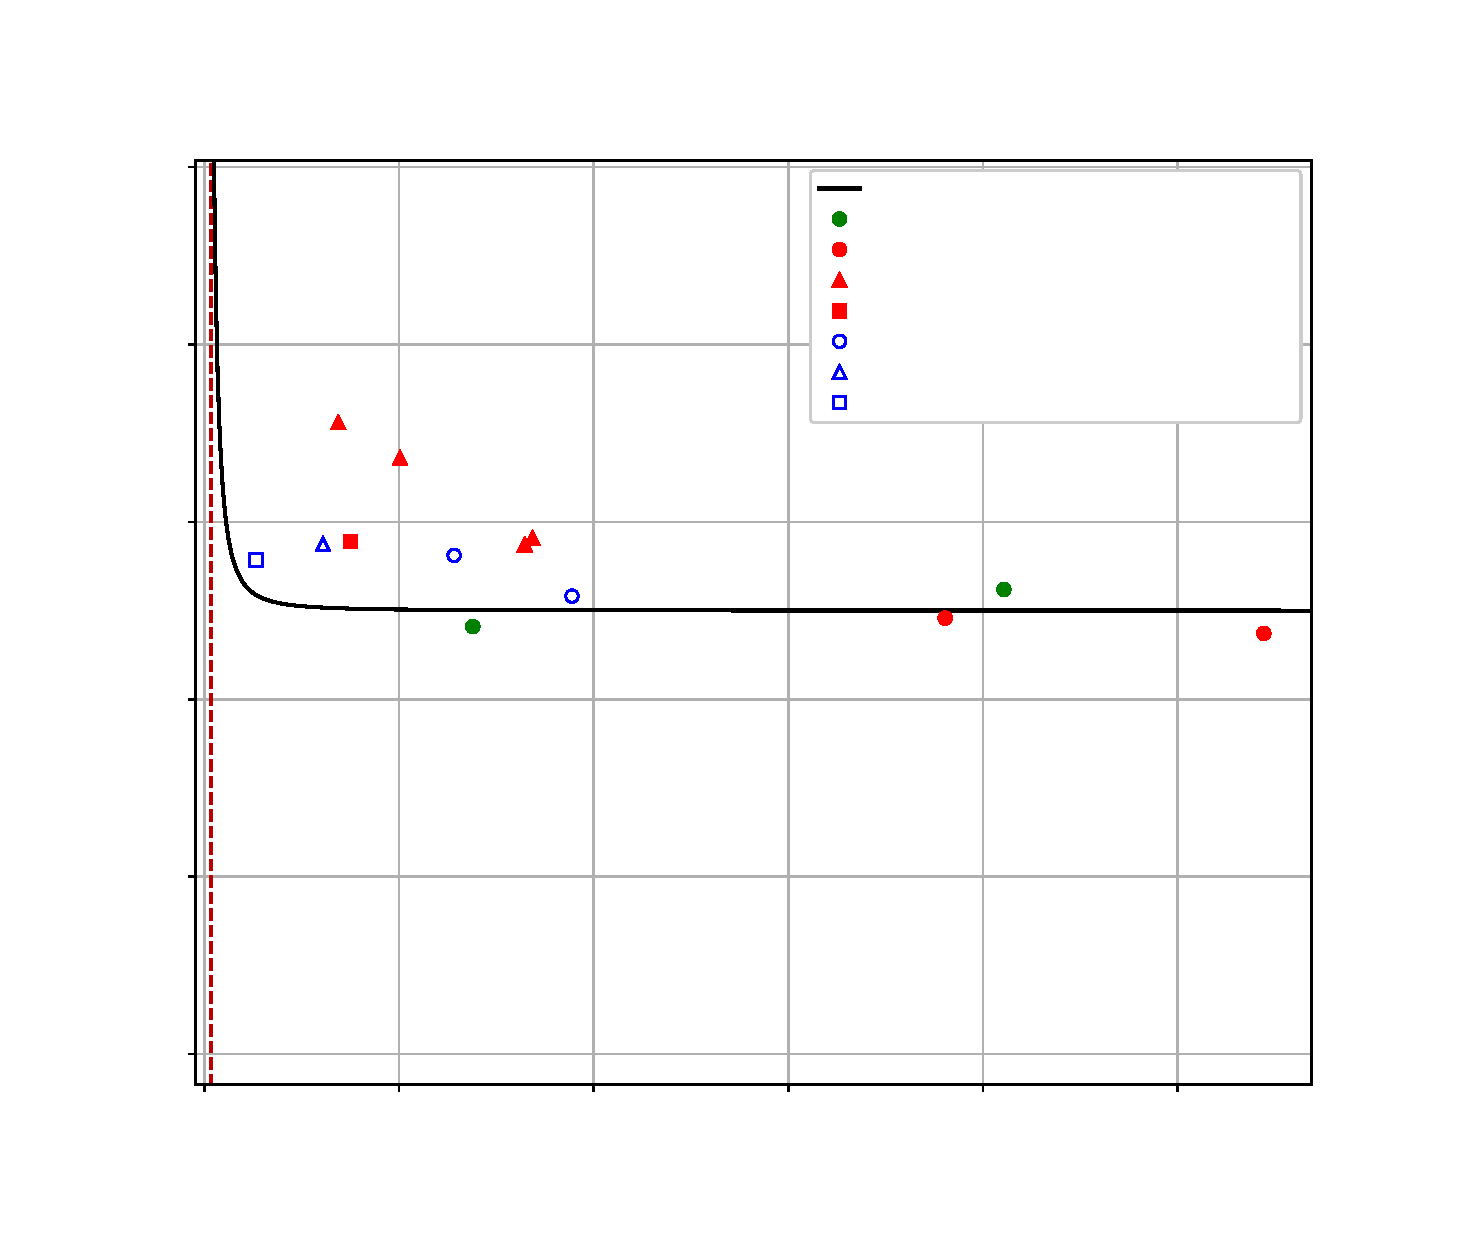
\includegraphics[width=\unitlength]{images_2ddl/yktol3.eps}}%
    \put(0.12,0.055061454){\color[rgb]{0,0,0}\makebox(0,0)[lb]{\smash{0}}}%
    \put(0.24650014,0.055061454){\color[rgb]{0,0,0}\makebox(0,0)[lb]{\smash{20}}}%
    \put(0.3817854,0.055061454){\color[rgb]{0,0,0}\makebox(0,0)[lb]{\smash{40}}}%
    \put(0.51707066,0.055061454){\color[rgb]{0,0,0}\makebox(0,0)[lb]{\smash{60}}}%
    \put(0.65235592,0.055061454){\color[rgb]{0,0,0}\makebox(0,0)[lb]{\smash{80}}}%
    \put(0.78303649,0.055061454){\color[rgb]{0,0,0}\makebox(0,0)[lb]{\smash{100}}}%
    \put(0.065107124,0.099723632){\color[rgb]{0,0,0}\makebox(0,0)[lb]{\smash{0.0}}}%
    \put(0.065107124,0.22054445){\color[rgb]{0,0,0}\makebox(0,0)[lb]{\smash{0.2}}}%
    \put(0.065107124,0.34385172){\color[rgb]{0,0,0}\makebox(0,0)[lb]{\smash{0.4}}}%
    \put(0.065107124,0.46716044){\color[rgb]{0,0,0}\makebox(0,0)[lb]{\smash{0.6}}}%
    \put(0.065107124,0.59046771){\color[rgb]{0,0,0}\makebox(0,0)[lb]{\smash{0.8}}}%
    \put(0.065107124,0.71377643){\color[rgb]{0,0,0}\makebox(0,0)[lb]{\smash{1.0}}}%
    \put(0.04226991,0.37966696){\color[rgb]{0,0,0}\rotatebox{90}{\makebox(0,0)[lb]{\smash{$E_{p,g}/E_{tot}$}}}}%
    \put(0.59802491,0.70735418){\color[rgb]{0,0,0}\makebox(0,0)[lb]{\smash{\scriptsize modèle théorique 2DDL}}}%
    \put(0.59802491,0.68610889){\color[rgb]{0,0,0}\makebox(0,0)[lb]{\smash{\scriptsize Y\&K acier (120,30)}}}%
    \put(0.59802491,0.6648636){\color[rgb]{0,0,0}\makebox(0,0)[lb]{\smash{\scriptsize Y\&K polyimide (125,10)}}}%
    \put(0.59802491,0.6436183){\color[rgb]{0,0,0}\makebox(0,0)[lb]{\smash{\scriptsize Y\&K polyimide (125,15)}}}%
    \put(0.59802491,0.62237446){\color[rgb]{0,0,0}\makebox(0,0)[lb]{\smash{\scriptsize Y\&K polyimide (125,20)}}}%
    \put(0.59802491,0.60112916){\color[rgb]{0,0,0}\makebox(0,0)[lb]{\smash{\scriptsize Y\&K polyimide (75,10)}}}%
    \put(0.59802491,0.57988387){\color[rgb]{0,0,0}\makebox(0,0)[lb]{\smash{\scriptsize Y\&K polyimide (75,15)}}}%
    \put(0.59802491,0.55863858){\color[rgb]{0,0,0}\makebox(0,0)[lb]{\smash{\scriptsize Y\&K polyimide (75,25)}}}%
    \put(0.47,0.01){\color[rgb]{0,0,0}\makebox(0,0)[lb]{\smash{$F/m_r g$ }}}%
  \end{picture}%
\endgroup%

\caption{Variation de l'efficacité énergétique en fonction du ratio $F/(m_r g)$ pour $\frac{\delta}{R}<0.35$. Les résultats sont en accord avec la courbe théorique.}
\label{fig:ytol}
\end{figure}


\subsection{Travail expérimental}             % Premier thème (Doctorat) ou "Détails de la Solution" (Maîtrise).
\Chapter{STABILITE DYNAMIQUE DU MOUVEMENT DE ROTATION D'UNE ROUE CYR}\label{sec:Theme2}

\section{Etude théorique}
\subsection{Description du mouvement}
On étudie ici le second mouvement caractéristique de la roue Cyr, analogue au mouvement du disque d'Euler. Le mouvement se découpe en deux phases, une première phase au cours de laquelle la roue décrit des cercles en roulant sur sa tranche, puis une deuxième phase où elle oscille en tournant de plus en plus vite avant de tomber à plat, stoppant net le mouvement. Ces deux phases correspondent à l'énchainement de deux figures de roue Cyr, la "roue" pour la phase 1 et la pièce pour la phase 2. \\
Ce qui suit est basé sur l'article de Batista \cite{Batista}, dont la démarche et le modèle mathématique développés pour le disque d'Euler ont été adaptés à la géométrie torique de la roue Cyr. De même que Batista, l'objectif est de développer des cartes de stabilité dynamiques, avec d'autres variables adaptées à notre cas.

\subsection{Hypothèses}
\begin{itemize}
    \item On se place en régime stationnaire: les variables qui prennent ainsi des valeurs constantes seront indicées d'un 0.
    \item On considère que la roue évolue sur un sol rugueux: il n'y a pas de glissement au niveau du point de contact.
    \item Le mouvement est étudié pour des valeurs de $\theta_0$ strictement comprises entre 0 et $\pi/2$ radians.
\end{itemize}

\subsection{Mise en équations}
\subsubsection{Variables et systèmes de coordonnées}

\begin{table}[htbp]
  \centering
  \caption{Constantes et variables des modèle analytiques}
  \begin{tabular}{|c|l|}
    \hline\rowcolor[gray]{0.8}\color{black}
    Symbole         & Description\\\hline
    
    $A$             & Point autour duquel la roue roule en dessinant des cercles\\
    $C$             & Centre de gravité de la roue\\
    $(F_x,F_y,F_z)$          & Composante de la force de réaction au point $P$ dans $C_{xzy}$ \\
    $(M_x,M_y,M_z)$          & Composante du moment de réaction au point $P$ dans $C_{xzy}$ \\
    $P$             & Point de contact entre la roue et le sol\\
    $R$             & Rayon médian de la roue\\
    $r_c$             & Rayon des cercles dessinés par la roue, obtenus par\\
    & projection du centre de masse au sol\\
    $(v_{Cx0},v_{Cy0},v_{Cz0})$           & Composantes de la vitesse du point C dans $C_{xzy}$ en régime permanent \\
    $(X_C,Y_C,Z_C)$           & Position du centre de gravité dans le reférentiel $OXYZ$\\
    $(\psi,\theta,\phi)$       & Position angulaire de la roue dans $OXYZ$\\
    
    $\Omega_0$          & Vitesse angulaire par rapport à l'axe Z en régime permanent\\
    $(\omega_{10},\omega_{20},\omega_{30})$          & Composantes de la vitesse angulaire $\vec{omega_0}$ dans $C{\xi \eta \zeta}$ en régime permanent\\\hline
    
    
  \end{tabular}
  \label{tab:batista}
\end{table}

On reprend les trois référentiels utilisés par Batista, schématisés en figures \ref{fig:ref1} et \ref{fig:ref2}: le référentiel fixe  $OXYZ$, et les référentiels mobiles $C_{xzy}$ et $C_{\xi\eta\zeta}$ ayant pour origine le centre de gravité de la roue. $C_{xzy}$ est décalé de $OXYZ$ par une rotation d'angle $\psi$ autour de l'axe $Z$ et $C_{\xi\eta\zeta}$ est décalee de $C_{xzy}$ par une rotation d'angle $\theta$ autour de l'axe $x$.

\begin{figure}[htb]
\centering
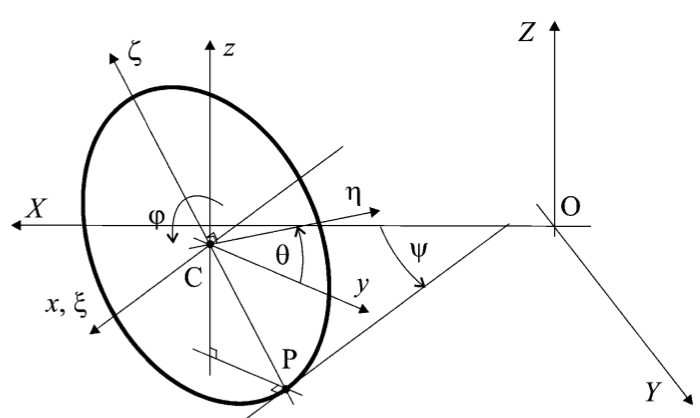
\includegraphics[width=4in]{batista/ref1.png}
\caption{Systèmes de coordonnées, tiré de l'article de Batista  \cite{Batista}. On utilise trois référentiels: un référentiel fixe, et deux référentiels liés à la roue, dont un correspond aux angles d'Euler.}
\label{fig:ref1}
\end{figure}

\begin{figure}[htb]
\centering
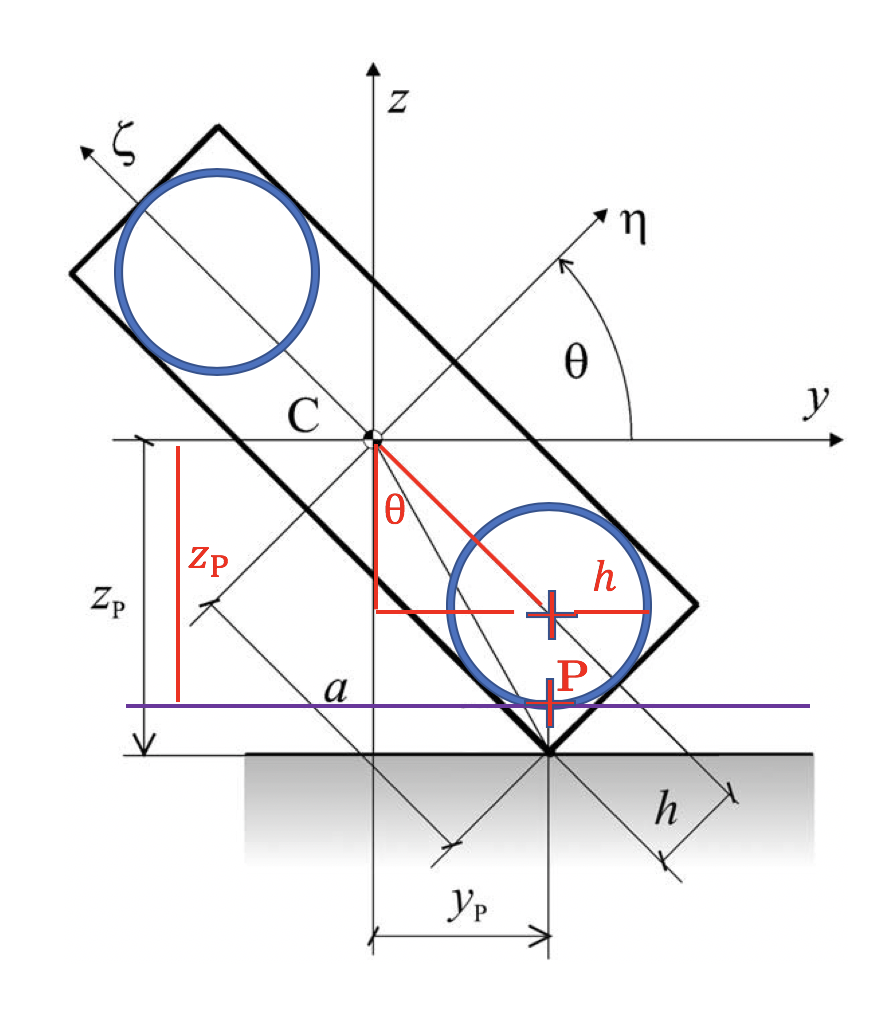
\includegraphics[width=3in]{batista/ref2.png}
\caption{Système de coordonnés, adapté de l'article de Batista \cite{Batista}. Nous étudions ici non pas un disque mais un tore, ce qui change, entre autres, l'expression de la position du point de contact $P$.}
\label{fig:ref2}
\end{figure}

\subsubsection{Equations}
On considère une roue à géométrie torique de rayon médian $R$ et de rayon externe de section $r_2$.\\
La position de la roue dans les référentiels présentés en figures \ref{fig:ref1} et \ref{fig:ref2} est décrite par les angles d'Euler: \\
$\theta$ décrit son inclinaison par rapport à la verticale: pour $\theta=\frac{\pi}{2}$, la roue est à plat sur le sol. \\
$\phi$ décrit la rotation de la roue, autour de son axe $\eta$, \\
$\psi$ décrit la rotation de la roue autour de l'axe $Z$ du référentiel fixe. \\

On se place en régime permanent: certaines des variables deviennent donc des constantes et seront indexées d'un zéro dans ce qui suit.
On note $(X_C,Y_C,Z_C)$ la position du centre de gravité dans le reférentiel $OXYZ$, $(v_{Cx0},v_{Cy0},v_{Cz0})$ les composantes de la vitesse du point C dans $C_{xzy}$, $(\omega_{10},\omega_{20},\omega_{30})$ les composantes de la vitesse angulaire $\vec{omega_0}$ dans $C{\xi \eta \zeta}$ et $\Omega$ la vitesse angulaire par rapport à l'axe $Z$.

Le mouvement de la roue est régie par les équations cinématiques suivantes \cite{Batista}:

 \begin{align} 
    \frac{dX_C}{dt} &=v_{Cx0} \cos{\psi}- v_{Cy0} \sin{\psi}  & \frac{d\psi}{dt}&=\Omega_0=\frac{\omega_{30}}{\cos{\theta_0}} \nonumber\\
    \frac{dY_C}{dt} &=v_{Cx0} \sin{\psi}- v_{Cy0} \cos{\psi} & \frac{d\theta}{dt}&=\omega_{10}=0 \nonumber\\
    \frac{dZ_C}{dt} &=v_{Cz0} & \frac{d\phi}{dt}&=\omega_{20}-\omega_{30} \tan{\theta_0}
    \label{eq:b1}
\end{align}



Les coordonnées du point de contact P dans C{xzy}, schématisé dans la figure \ref{fig:ref2} s'expriment:
\begin{align}
    x_P&=0 \nonumber\\
    y_P&=R\sin{\theta_0} \nonumber\\
    z_P&=-R\cos{\theta_0}-r_2
  \label{eq:b2}
\end{align}

D'après la règle de transport des torseurs, la vitesse du point de contact dans $C_{xzy}$ s'écrit:
\begin{equation}
    \vec{v_{P0}}=\vec{v_{C0}}+\vec{\omega_0} \wedge \vec{CP},
  \label{eq:b3}
\end{equation}

avec $\vec{\omega_0}=(\omega_{10},\omega_{20},\omega_{30})$
et $\vec{CP}=(0,R\sin{\theta_0},-R\cos{\theta_0}-r_2)$ .



Les composantes de la vitesse au point de contact dans $C_{xzy}$ s'écrivent donc:
\begin{align}
    v_{Px_0}&=v_{Cx_0}-\omega_{20} (R\cos{\theta_0}+r_2) -\omega_{30} R\sin{\theta} \nonumber \\
    v_{Py_0}&=v_{Cy_0} + \omega_{10} (R\cos{\theta_0}+r_2)= v_{Cy_0} \nonumber\\
    v_{Pz_0}&=v_{Cz_0} + \omega_{10} R\sin{\theta_0} = v_{Cz_0}
  \label{eq:b4}
\end{align}

On a fait l'hypothèse d'un sol rugueux: on a donc $v_{Px0}=v_{Py0}=0$, et comme le contact entre le sol et la roue est permanent, $v_{Pz0}=0=v_{Cz_0}$.


Les composantes de l'accélération du centre d'inertie de la roue dans $C{xzy}$ s'expriment à partir de l'équation \ref{eq:b1} projetée dans $C{xzy}$:

\begin{align}
    a_{Cx0}&=\frac{dv_{Cx0}}{dt}-\Omega_0 v_{Cy0}=-\Omega_0 v_{Cy0} \nonumber\\
    a_{Cy0}&=\frac{dv_{Cy0}}{dt} + \Omega_0 v_{Cx0}=\Omega_0 v_{Cx0}\nonumber\\
    a_{Cz0}&=\frac{dv_{Cz0}}{dt} = 0
  \label{eq:b5}
\end{align}

L'équation \ref{eq:b5} combinée à la relation fondamentale de la dynamique en translation donne:

\begin{align}
    m_r\Omega_0 v_{Cy0}&=-F_x \nonumber\\
    m_r \Omega_0 v_{Cx0}&=F_y \nonumber\\
    m_r(\frac{dv_{Cz0}}{dt})&=-mg+F_z=0,
  \label{eq:b7}
\end{align}

où $F_x$, $F_y$ et $F_z$ sont les composantes de la force de réaction $\mathbf{F}$ au point P, exprimées dans $C_{xyz}$.

Le moment cinétique au centre de masse s'exprime $\vec{L_{C0}}=I \cdot \vec{\omega}$, avec pour tenseur d'inertie:
\begin{equation}
    I=
\begin{pmatrix}
   m_r (\frac{1}{2}R^2+\frac{5}{8}r_2^2) & 0  &  0 \\
  0 &  m_r(R^2+\frac{3}{4}r_2^2) & 0 \\
  0 & 0 & m_r (\frac{1}{2}R^2+\frac{5}{8}r_2^2)
\end{pmatrix}
\label{eq:inertie}
\end{equation}


Notons $k_1^2=\frac{1}{2}R^2+\frac{5}{8}r_2^2$ et $k_2^2=R^2+\frac{3}{4}r_2^2$

Les composantes du moment cinétique en $C$ dans $C_{\xi \eta \zeta}$ s'écrivent donc:
\begin{align}
    L_{C\xi0 }&=m_r k_1^2 \omega_{10}=0 \nonumber\\
    L_{C\eta0}&=m_r k_2^2 \omega_{20} \nonumber\\
    L_{C\zeta0 }&=m_r k_1^2 \omega_{30}
  \label{eq:b6}
\end{align}

La relation fondamentale de la dynamique en rotation appliquée au centre de masse de la roue dans le référentiel $C_{xyz}$ donne:

\begin{equation}
    \frac{d \mathbf{L_{C0}}}{dt} + \mathbf{R} \wedge \mathbf{L_{C0}} = \mathbf{M}+ \overrightarrow{CP} \wedge \mathbf{F} 
\label{eq:rfdr}
\end{equation}

où $\mathbf{R}$ est la vitesse angulaire de $C_{\xi \eta \zeta}$ et $\mathbf{M}$ est le moment de réaction au point P exprimé dans $C_{xyz}$, de composantes $M_x$, $M_y$ et $M_z$.

Le référentiel $C_{\xi \eta \zeta}$ a été défini de telle sorte que sa vitesse angulaire $\mathbf{R}$ est égale à la vitesse angulaire $\mathbf{\omega}$ de la roue sans la rotation en $\phi$ autour de l'axe $\eta$.

On a donc
\begin{equation}
   \mathbf{R}= \begin{pmatrix}
    \omega_1  \\
    \omega_2 - \frac{d\phi}{dt} \\
    \omega_3     
\end{pmatrix} 
=
\begin{pmatrix}
    \omega_1  \\
    \omega_{3}\tan(\theta) \\
    \omega_3     
\end{pmatrix} 
\label{eq:rb}
\end{equation}

En régime permanent, \ref{eq:rb} devient:

\begin{equation}
   \mathbf{R}= \begin{pmatrix}
    0  \\
    \omega_{30}\tan(\theta_0) \\
    \omega_{30}     
\end{pmatrix} 
\label{eq:rb2}
\end{equation}

En substituant \ref{eq:b6} et \ref{eq:rb2} dans \ref{eq:rfdr}, on obtient:

\begin{align}
    m_r(k_2^2\omega_{20}-k_1^2\omega_{30} \tan{\theta_0})\omega_{30} +(R\cos{\theta_0}+r_2)F_y + R\sin{\theta_0}F_z + M_x &=0 \nonumber\\
    -(R+r_2)F_x + M_y \cos{\theta_0} +M_z \sin{\theta_0}&=0 \nonumber\\
    m_r(-k_2^2\omega_{20}+k_1^2\omega_{30} \tan{\theta_0})\omega_{10} + hF_x - M_y \sin{\theta_0} +M_z \cos{\theta_0}&=0
  \label{eq:b8}
\end{align}

La dérivée de l'énergie mécanique s'exprime: 
\begin{equation}
    \frac{dE}{dt}=P_F + P_M, 
    \label{eq:be1}
\end{equation}

avec $P_F$ et $P_M$, les puissances de la fore de réaction $F$ et du moment de réaction $M$, ce qui donne:

\begin{equation}
    \frac{dE}{dt}=\vec{v_P} \cdot \vec{F} + \vec{\omega} \cdot \vec{M}
    \label{eq:be2}
\end{equation}

En régime stationnaire, on a $\dfrac{dE}{dt}=0$, et comme on a fait l'hypothèse du sol rugueux, $\vec{v_P}=\vec{0}$, \ref{eq:be2} devient donc: $$\vec{\omega} \cdot \vec{M}$$

Le disque doit avoir une vitesse de rotation pour qu'il y ait un mouvement à étudier, on en déduit donc $\vec{M}=\vec{0}$

Les équations \ref{eq:b7} et \ref{eq:b8} deviennent alors:

\begin{align}
    &F_y=m_r \Omega_0 v_{Cx0} \nonumber\\
    &m_r(k_2^2\omega_{20}-k_1^2\omega_{30} \tan{\theta_0})\omega_{30} +(R\cos{\theta_0}+r_2)m_r \Omega_0 v_{Cx0} + R\sin{\theta_0}mg =0
  \label{eq:b9}
\end{align}

Or, on sait de l'équation \ref{eq:b1} que:

\begin{align}
    \omega_{20}&=\omega_0 + \Omega_0 \sin{\theta_0} \nonumber\\
    \omega_{30}&=\Omega_0 \cos{\theta_0},
  \label{eq:b10}
\end{align}

et de l'équation \ref{eq:b2} que:

\begin{equation}
    v_{Cx0}=(R+r_2)\omega_{20}-r_2\omega_{30}
    \label{eq:b10b}
\end{equation}

En substituant \ref{eq:b10} et \ref{eq:b11} dans \ref{eq:b9}, on obtient:

\begin{align}
     &m_r(k_2^2(\omega_0 + \Omega_0 \sin{\theta_0})-k_1^2(\Omega_0 \cos{\theta_0}) \tan{\theta_0})(\Omega_0 \cos{\theta_0})  \nonumber\\
    &+(R\cos{\theta_0}+r_2)m_r \Omega_0 ((R+r_2)(\omega_0 + \Omega_0 \sin{\theta_0})-r_2\Omega_0 \cos{\theta_0}) + R\sin{\theta_0}m_r g =0
  \label{eq:b11}
\end{align}

soit

\begin{align}
     &[(k_2^2-k_1^2)\sin(\theta_0)\cos(\theta_0)+(R \cos(\theta_0)+r_2)[(R+r_2)\sin(\theta_0)-r_2 \cos(\theta_0)]]\Omega_0^2 \nonumber\\
     &+\omega_0[k_2^2 \cos(\theta_0)+(R+r_2)(R \cos(\theta_0))] \Omega_0 + R g \sin(\theta_0) =0
  \label{eq:b12}
\end{align}

On définit la longueur adimensionnelle $$\hat{L}=\dfrac{\sqrt{(k_2^2-k_1^2)\sin(\theta_0)\cos(\theta_0)+(R \cos(\theta_0)+r_2)[(R+r_2)\sin(\theta_0)-r_2 \cos(\theta_0)]}}{R\sin{\theta_0}}$$,
et la pulsation adimensionnelle $\hat{\omega_0}=\omega_0 \sqrt{\dfrac{R+r_2}{g}}$.

Ecrit sous forme adimensionnelle, \ref{eq:b12} devient:

\begin{equation}
 \begin{split}
     \frac{R \sin(\theta_0)\hat{L}^2}{g} \Omega_0^2+\hat{\omega_0} \frac{k_2^2+R(R+r_2)}{R \tan(\theta_0) \sqrt{g(R+r_2)}} \Omega_0+1 =0
 \end{split}
  \label{eq:b12a}
\end{equation}

L'équation \ref{eq:b11} se traduit ainsi: pour que le régime stationnaire puisse exister, l'équation polynomiale en $\Omega_0$ doit avoir une solution réelle. L'existence de cette solution dépend des valeurs de $(\theta_0,\omega_0)$. On peut ainsi tracer une première partie de la carte de stabilité, en séparant graphiquement les cas où le régime stationnaire est possible, et les cas où il ne peut pas exister.

\begin{equation}
 \Omega_0=g \frac{\hat{\omega_0} \frac{k_2^2+R(R+r_2)}{R \tan(\theta_0) \sqrt{g(R+r_2)}}\pm \sqrt{\Delta}}{2R\sin(\theta_0)\hat{L}^2},
  \label{eq:b13}
\end{equation}

avec 

\begin{equation}
 \Delta=(\hat{\omega_0} \frac{k_2^2+R(R+r_2)}{R \tan(\theta_0) \sqrt{g(R+r_2)}})^2-4\frac{ \hat{L}^2 R \sin(\theta_0)}{g}
  \label{eq:b14}
\end{equation}

Pour que $\Omega_0$ soit réel, il faut $\Delta \geq 0$
Lorsque $\Delta < 0$ l'équilibre n'existe pas

La frontière de l'équilibre dynamique est décrite par l'équation:

\begin{equation}
(\hat{\omega_0} \frac{k_2^2+R(R+r_2)}{R \tan(\theta_0) \sqrt{g(R+r_2)}})^2-4\frac{ \hat{L}^2 R \sin(\theta_0)}{g} = 0
\label{eq:b15}
\end{equation}

Ce qui équivaut à:

\begin{equation}
 \hat{\omega_0}= \pm \frac{2\hat{L} R \tan(\theta_0) \sqrt{R(R+r_2)\sin(\theta_0)}}{k_2^2+R(R+r_2)}
  \label{eq:b16}
\end{equation}

Lorsque $$ |\hat{\omega_0}| < \frac{2\hat{L} R \tan(\theta_0) \sqrt{R(R+r_2)\sin(\theta_0)}}{k_2^2+R(R+r_2)},
$$
 la force centrifuge et la réaction du sol ne peuvent plus contrebalancer l'effet de la gravité.
 
\begin{figure}[h]
\centering
\def\svgwidth{370}
%% Creator: Inkscape inkscape 0.92.2, www.inkscape.org
%% PDF/EPS/PS + LaTeX output extension by Johan Engelen, 2010
%% Accompanies image file 'bat12.eps' (pdf, eps, ps)
%%
%% To include the image in your LaTeX document, write
%%   \input{<filename>.pdf_tex}
%%  instead of
%%   \includegraphics{<filename>.pdf}
%% To scale the image, write
%%   \def\svgwidth{<desired width>}
%%   \input{<filename>.pdf_tex}
%%  instead of
%%   \includegraphics[width=<desired width>]{<filename>.pdf}
%%
%% Images with a different path to the parent latex file can
%% be accessed with the `import' package (which may need to be
%% installed) using
%%   \usepackage{import}
%% in the preamble, and then including the image with
%%   \import{<path to file>}{<filename>.pdf_tex}
%% Alternatively, one can specify
%%   \graphicspath{{<path to file>/}}
%% 
%% For more information, please see info/svg-inkscape on CTAN:
%%   http://tug.ctan.org/tex-archive/info/svg-inkscape
%%


\begingroup%
  \makeatletter%
  \providecommand\color[2][]{%
    \errmessage{(Inkscape) Color is used for the text in Inkscape, but the package 'color.sty' is not loaded}%
    \renewcommand\color[2][]{}%
  }%
  \providecommand\transparent[1]{%
    \errmessage{(Inkscape) Transparency is used (non-zero) for the text in Inkscape, but the package 'transparent.sty' is not loaded}%
    \renewcommand\transparent[1]{}%
  }%
  \providecommand\rotatebox[2]{#2}%
  \ifx\svgwidth\undefined%
    \setlength{\unitlength}{432bp}%
    \ifx\svgscale\undefined%
      \relax%
    \else%
      \setlength{\unitlength}{\unitlength * \real{\svgscale}}%
    \fi%
  \else%
    \setlength{\unitlength}{\svgwidth}%
  \fi%
  \global\let\svgwidth\undefined%
  \global\let\svgscale\undefined%
  \makeatother%
  \begin{picture}(1,0.83333333)%
    \put(0,0){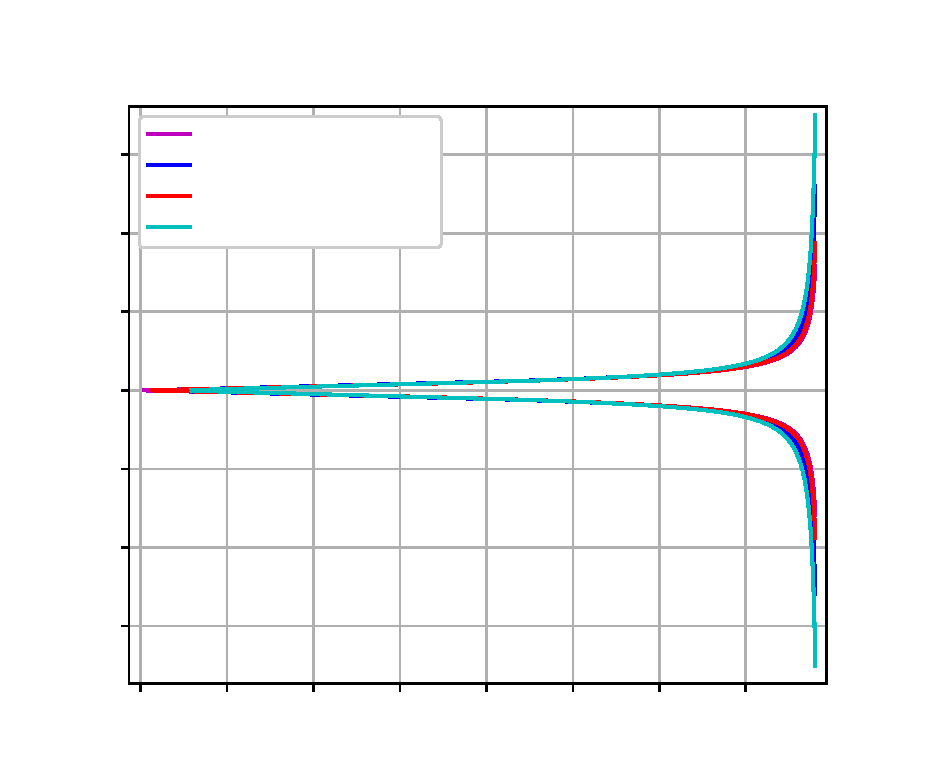
\includegraphics[width=\unitlength]{imagesbat/bat12.eps}}%
    \put(0.11923819,0.05788495){\color[rgb]{0,0,0}\makebox(0,0)[lb]{\smash{0.0}}}%
    \put(0.21531203,0.05788495){\color[rgb]{0,0,0}\makebox(0,0)[lb]{\smash{0.2}}}%
    \put(0.31138425,0.05788495){\color[rgb]{0,0,0}\makebox(0,0)[lb]{\smash{0.4}}}%
    \put(0.40745832,0.05788495){\color[rgb]{0,0,0}\makebox(0,0)[lb]{\smash{0.6}}}%
    \put(0.50353008,0.05788495){\color[rgb]{0,0,0}\makebox(0,0)[lb]{\smash{0.8}}}%
    \put(0.59960415,0.05788495){\color[rgb]{0,0,0}\makebox(0,0)[lb]{\smash{1.0}}}%
    \put(0.69567822,0.05788495){\color[rgb]{0,0,0}\makebox(0,0)[lb]{\smash{1.2}}}%
    \put(0.79174998,0.05788495){\color[rgb]{0,0,0}\makebox(0,0)[lb]{\smash{1.4}}}%
    \put(0.05,0.14706226){\color[rgb]{0,0,0}\makebox(0,0)[lb]{\smash{$-30$}}}%
    \put(0.05,0.23435879){\color[rgb]{0,0,0}\makebox(0,0)[lb]{\smash{$-20$}}}%
    \put(0.05,0.3216574){\color[rgb]{0,0,0}\makebox(0,0)[lb]{\smash{$-10$}}}%
    \put(0.09407546,0.40895601){\color[rgb]{0,0,0}\makebox(0,0)[lb]{\smash{0}}}%
    \put(0.07935486,0.49625462){\color[rgb]{0,0,0}\makebox(0,0)[lb]{\smash{10}}}%
    \put(0.07935486,0.58355323){\color[rgb]{0,0,0}\makebox(0,0)[lb]{\smash{20}}}%
    \put(0.07935486,0.67084952){\color[rgb]{0,0,0}\makebox(0,0)[lb]{\smash{30}}}%
    \put(0.470353008,0.01){\color[rgb]{0,0,0}\makebox(0,0)[lb]{\smash{ $\theta_0 (rad)$}}}%
    \put(0.04524745,0.4){\color[rgb]{0,0,0}\rotatebox{90}{\makebox(0,0)[lb]{\smash{$\hat{\omega_0} $}}}}%
    \put(0.21064814,0.69492128){\color[rgb]{0,0,0}\makebox(0,0)[lb]{\smash{\footnotesize $R=1.0 m, r_2=1.0 cm$}}}%
    \put(0.21064814,0.66030785){\color[rgb]{0,0,0}\makebox(0,0)[lb]{\smash{\footnotesize $R=1.0 m, r_2=5.0 cm$}}}%
    \put(0.21064814,0.62569443){\color[rgb]{0,0,0}\makebox(0,0)[lb]{\smash{\footnotesize $R=0.5 m, r_2=1.0 cm$}}}%
    \put(0.21064814,0.591081){\color[rgb]{0,0,0}\makebox(0,0)[lb]{\smash{\footnotesize $R=0.5 m, r_2=5.0 cm$}}}%
    \put(0.59960415,0.23435879){\color[rgb]{0,0,0}\makebox(0,0)[lb]{\smash{stable}}}%
    \put(0.59960415,0.58355323){\color[rgb]{0,0,0}\makebox(0,0)[lb]{\smash{stable}}}%
    \put(0.75,0.40895601){\color[rgb]{0,0,0}\makebox(0,0)[lb]{\smash{instable}}}%
  \end{picture}%
\endgroup%

\caption{Première partie de la carte de stabilité. La frontière détermine l'existence d'une position d'équilibre dynamique pour chaque couple ($\theta_0,\hat{\omega_0}$), où $\hat{\omega_0}$ correspond à la vitesse de rotation adimensionnelle, $\hat{\omega_0}=\omega_0 \sqrt{\dfrac{R+r_2}{g}}$}
\end{figure}

\section{Réponse à une perturbation}

On étudie à présent la réponse du système en régime permanent à une petite perturbation, ce qui se traduit par l'ajout d'un terme de pulsation $\sigma$ aux variables $\theta, \omega_1, \omega_2, \omega_3$: \\


\begin{align}
 \theta&=\theta_0 + \epsilon \Tilde{\theta} e^{i \sigma t} \nonumber\\
 \omega_1&= \omega_{10} + \epsilon \Tilde{\omega_1} e^{i \sigma t} = \epsilon \Tilde{\omega_1} e^{i \sigma t} = \frac{d\theta }{dt} \nonumber\\
 \omega_2&= \omega_{20} + \epsilon \Tilde{\omega_2} e^{i \sigma t} \nonumber\\
 \omega_3&= \omega_{30} + \epsilon \Tilde{\omega_3} e^{i \sigma t}
  \label{eq:b17}
\end{align}

Avec les variables \ref{eq:b17}, les coordonnées du point de contact P dans C{xzy}, schématisé dans la figure \ref{fig:ref2} s'expriment à présent:
\begin{align}
    x_P&=0 \nonumber\\
    y_P&=R\sin{\theta} \nonumber\\
    z_P&=-R\cos{\theta}-r_2.
  \label{eq:b2p}
\end{align}

Et les composantes de la vitesse angulaire deviennent:

\begin{equation}
    \vec{\omega}=(\omega_1,\omega_2,\omega_3)
    \label{eq:b3p}
\end{equation}

En substituant \ref{eq:b2p} et \ref{eq:b3p} dans \ref{eq:b3}, et en conservant l'hypothèse d'un sol parfaitement rugueux ($\vec{v_P}=\vec{0}$) on obtient la nouvelle expression des composantes de la vitesse du centre de gravité dans $C_{xzy}$:

\begin{align}
    v_{Cx}&=(R\cos(\theta)+r_2)\omega_2+R \sin(\theta)\omega_3 \nonumber\\
    v_{Cy} &= -(R\cos(\theta)+r_2)\omega_1 \nonumber\\
    v_{Cz} &= -R \sin(\theta)\omega_1
  \label{eq:b18}
\end{align}

En simplifiant \ref{eq:b18} avec les développements limités \ref{eq:bdl}, en ne gardant que les termes d'ordre 1 en $\epsilon$, on obtient \ref{eq:b18b}:

\begin{align}
    \cos(\theta_0 + \epsilon \Tilde{\theta} e^{i \sigma t})&=\cos(\theta_0)- \sin(\theta_0)\epsilon \Tilde{\theta} e^{i \sigma t} + o(\epsilon) \nonumber\\
    \sin(\theta_0 + \epsilon \Tilde{\theta} e^{i \sigma t})&=\sin(\theta_0)+ \cos(\theta_0)\epsilon \Tilde{\theta} e^{i \sigma t} + o(\epsilon)\nonumber\\
    \tan(\theta_0 + \epsilon \Tilde{\theta} e^{i \sigma t})&=\tan(\theta_0)+ (1+\tan(\theta_0)^2)\epsilon \Tilde{\theta} e^{i \sigma t} + o(\epsilon)
\label{eq:bdl}
\end{align}

\begin{align}
    v_{Cx}=&(R\cos(\theta_0)+r_2)\omega_{20}+R \sin{\theta_0}\omega_{30} \nonumber\\ 
    &+ \epsilon e^{i \sigma t}[(R\cos(\theta_0)+r_2) \Tilde{\omega_2} +R(\omega_{30}\cos(\theta_0)-\sin(\theta_0)\omega_{20}) \Tilde{\theta}+R\sin(\theta_0) \Tilde{\omega_3} ] \nonumber\\ 
    v_{Cy} =& -(R\cos(\theta_0)+r_2)\epsilon \Tilde{\omega_1} e^{i \sigma t} \nonumber\\ 
    v_{Cz} =& -R \sin(\theta_0)\epsilon \Tilde{\omega_1} e^{i \sigma t}
  \label{eq:b18b}
\end{align}

Les composantes de l'accélération du centre d'inertie de la roue dans $C{xzy}$ s'expriment à partir de l'équation \ref{eq:b1} projetée dans $C{xzy}$:

\begin{align}
    a_{Cx}&=\frac{dv_{Cx}}{dt}-\Omega v_{Cy} \nonumber\\
    a_{Cy}&=\frac{dv_{Cy}}{dt} + \Omega v_{Cx}\nonumber\\
    a_{Cz}&=\frac{dv_{Cz}}{dt} 
  \label{eq:b19b}
\end{align}
\\
L'équation \ref{eq:b1}, permet d'exprimer $\Omega$:
\begin{equation}
    \Omega=\frac{\omega_{30}}{\cos{\theta_0}} + (\frac{\tilde{\omega_3}}{\cos(\theta_0)}+\frac{\sin(\theta_0)}{\cos(\theta_0)^2}\omega_{30}\tilde{\theta})\epsilon e^{i \sigma t}
    \label{eq:Omega}
\end{equation}


En substituant \ref{eq:b18b} à l'intérieur de \ref{eq:b19b}, on obtient:

\begin{align}
    a_{Cx}=& i \sigma \epsilon e^{i \sigma t}[(R\cos(\theta_0)+r_2) \Tilde{\omega_2} +R(\omega_{30}\cos(\theta_0)-\sin(\theta_0)\omega_{20}) \Tilde{\theta}+R\sin(\theta_0) \Tilde{\omega_3} ] \nonumber\\
    &+\Omega (R\cos(\theta_0)+r_2)\epsilon \Tilde{\omega_1} e^{i \sigma t} \nonumber\\
    a_{Cy}=& -i \sigma( R\cos(\theta_0)+r_2)\epsilon \Tilde{\omega_1} e^{i \sigma t} 
    + \Omega [(R\cos(\theta_0)+r_2)\omega_{20}+R \sin{\theta_0}\omega_{30} \nonumber\\ 
    &+ \epsilon e^{i \sigma t}[(R\cos(\theta_0)+r_2) \Tilde{\omega_2} +R(\omega_{30}\cos(\theta_0)-\sin(\theta_0)\omega_{20}) \Tilde{\theta}+R\sin(\theta_0) \Tilde{\omega_3} ] ]\nonumber \\
    a_{Cz}=& -i \sigma R \sin(\theta_0)\epsilon \Tilde{\omega_1} e^{i \sigma t} 
  \label{eq:b19b2}
\end{align}

D'après \ref{eq:b19b2} et la relation fondamentale de la dynamique en translation:

\begin{align}
  i \sigma \epsilon e^{i \sigma t}[(R\cos(\theta_0)+r_2) \Tilde{\omega_2} +R(\omega_{30}\cos(\theta_0)-\sin(\theta_0)\omega_{20}) \Tilde{\theta}+R\sin(\theta_0) \Tilde{\omega_3} ]& \nonumber \\
    +\Omega (R\cos(\theta_0)+r_2)\epsilon \Tilde{\omega_1} e^{i \sigma t}&=\frac{F_x}{m_r} \nonumber \\
    -i \sigma( R\cos(\theta_0)+r_2)\epsilon \Tilde{\omega_1} e^{i \sigma t}
    + \Omega [(R\cos(\theta_0)+r_2)\omega_{20}+R \sin{\theta_0}\omega_{30}& \nonumber\\ 
    + \epsilon e^{i \sigma t}[(R\cos(\theta_0)+r_2) \Tilde{\omega_2} +R(\omega_{30}\cos(\theta_0)-\sin(\theta_0)\omega_{20}) \Tilde{\theta}+R\sin(\theta_0) \Tilde{\omega_3} ] ]&=\frac{F_y}{m_r} \nonumber \\
    -i \sigma R \sin(\theta_0)\epsilon \Tilde{\omega_1} e^{i \sigma t}&=- g +\frac{F_z}{m_r}
  \label{eq:b20}
\end{align}

Le moment cinétique au centre de masse s'exprime $\vec{L_{C}}=I \cdot \vec{\omega}$, le tenseur d'inertie étant donné en \ref{eq:inertie}.

Les composantes du moment cinétique dans $C_{\xi \eta \zeta}$ s'écrivent donc:
\begin{align}
    L_{C\xi }&=m_r k_1^2 \omega_{1} \nonumber\\
    L_{C\eta}&=m_r k_2^2 \omega_{2} \nonumber\\
    L_{C\zeta }&=m_r k_1^2 \omega_{3}
  \label{eq:b6b}
\end{align}

La relation fondamentale de la dynamique en rotation appliquée au centre de masse de la roue dans le référentiel $C_{xyz}$ donne:

\begin{equation}
    \frac{d \mathbf{L_{C}}}{dt} + \mathbf{R} \wedge \mathbf{L_{C}} = \mathbf{M}+ \overrightarrow{CP} \wedge \mathbf{F} 
\label{eq:rfdr2}
\end{equation}

où $\mathbf{R}$ est la vitesse angulaire de $C_{\xi \eta \zeta}$ et $\mathbf{M}$ est le moment de réaction au point P exprimé dans $C_{xyz}$, de composantes $M_x$, $M_y$ et $M_z$.

L'expression de $\mathbf{R}$ a été déterminée en \ref{eq:rb}

\begin{equation}
   \mathbf{R}= 
\begin{pmatrix}
    \omega_1  \\
    \omega_{3}\tan(\theta) \\
    \omega_3     
\end{pmatrix} 
\label{eq:rb3}
\end{equation}

En substituant \ref{eq:b6b} et \ref{eq:rb3} dans \ref{eq:rfdr2}, on obtient:

\begin{align}
    k_1^2\frac{d\omega_1}{dt} &=(k_2^2\omega_2-k_1^2\omega_3 \tan{\theta})\omega_3+(R\cos{\theta}+r_2)\frac{F_y}{m_r}+ R\sin{\theta}\frac{F_z}{m_r} \nonumber \\
    k_2^2\frac{d\omega_2}{dt} &=-(R+r_2) \frac{F_x}{m_r} \nonumber \\
    k_1^2\frac{d\omega_3}{dt} &=(-k_2^2\omega_2+k_1^2\omega_3 \tan(\theta))\omega_1 + r_2 \frac{F_x}{m_r}
  \label{eq:b21}
\end{align}

On substitue \ref{eq:b17} dans \ref{eq:b21}, en simplifiant les expressions à l'aide de développements limités et on néglige les termes de perturbation d'ordre supérieur ou égal à 2.

\begin{align}
    k_1^2 i \sigma\epsilon \Tilde{\omega_1} e^{i \sigma t} =&(k_2^2\omega_{20}-k_1^2\omega_{30} \tan{\theta_0})\omega_{30}+\epsilon e^{i\sigma t}[k_2^2 \omega_{20} \tilde{\omega_3}+k_2^2 \omega_{30} \tilde{\omega_2} -2k_1^2\omega_{30} \tan(\theta_0)\tilde{\omega_3} \nonumber\\
    &-k_1^2 \omega_{30}^2(1+\tan(\theta_0)^2)\tilde{\theta} ]+(R(\cos(\theta_0)- \sin(\theta_0)\epsilon \Tilde{\theta} e^{i \sigma t})+r_2)\frac{F_y}{m_r}\nonumber \\
    &+ R(\sin(\theta_0)+ \cos(\theta_0)\epsilon \Tilde{\theta} e^{i \sigma t})\frac{F_z}{m_r} \nonumber\\ 
    k_2^2 i \sigma\epsilon \Tilde{\omega_2} e^{i \sigma t}=&-(R+r_2) \frac{F_x}{m_r} \nonumber\\ 
    k_1^2 i \sigma\epsilon \Tilde{\omega_3} e^{i \sigma t}=&(-k_2^2\omega_{20}+k_1^2\omega_{30} \tan(\theta_0))\epsilon \Tilde{\omega_1} e^{i \sigma t} + r_2 \frac{F_x}{m_r}
  \label{eq:b22}
\end{align}

On substitue ensuite \ref{eq:b20} et \ref{eq:Omega} dans \ref{eq:b22} 

\begin{align}
    k_1^2 i \sigma \epsilon \Tilde{\omega_1} e^{i \sigma t} =&(k_2^2\omega_{20}-k_1^2\omega_{30} \tan{\theta_0})\omega_{30}+\epsilon e^{i\sigma t}[k_2^2 \omega_{20} \tilde{\omega_3}+k_2^2 \omega_{30} \tilde{\omega_2} -2k_1^2\omega_{30} \tan(\theta_0)\tilde{\omega_3}\nonumber\\
    &-k_1^2 \omega_{30}^2(1+\tan(\theta_0)^2)\tilde{\theta} ]+(R(\cos(\theta_0)- \sin(\theta_0)\epsilon \Tilde{\theta} e^{i \sigma t})+r_2)[-i \sigma( R\cos(\theta_0)+r_2)\epsilon \Tilde{\omega_1} e^{i \sigma t} \nonumber\\
    &+ (\frac{\omega_{30}}{\cos{\theta_0}} + (\frac{\tilde{\omega_3}}{\cos(\theta_0)}+\frac{\sin(\theta_0)}{\cos(\theta_0)^2}\omega_{30}\tilde{\theta})\epsilon e^{i \sigma t}) [(R\cos(\theta_0)+r_2)\omega_{20}+R \sin{\theta_0}\omega_{30} \nonumber\\ 
    &+ \epsilon e^{i \sigma t}[(R\cos(\theta_0)+r_2) \Tilde{\omega_2} +R(\omega_{30}\cos(\theta_0)-\sin(\theta_0)\omega_{20}) \Tilde{\theta}+R\sin(\theta_0) \Tilde{\omega_3} ] ]] \nonumber\\
    &+ R(\sin(\theta_0)+ \cos(\theta_0)\epsilon \Tilde{\theta} e^{i \sigma t})[g-i \sigma R \sin(\theta_0)\epsilon \Tilde{\omega_1} e^{i \sigma t}] \nonumber\\
    k_2^2 i \sigma\epsilon \Tilde{\omega_2} e^{i \sigma t}=&-(R+r_2) [i \sigma \epsilon e^{i \sigma t}[(R\cos(\theta_0)+r_2) \Tilde{\omega_2} +R(\omega_{30}\cos(\theta_0)-\sin(\theta_0)\omega_{20}) \Tilde{\theta}+R\sin(\theta_0) \Tilde{\omega_3} ] \nonumber\\
    &+\frac{\omega_{30}}{\cos{\theta_0}} (R\cos(\theta_0)+r_2)\epsilon \Tilde{\omega_1} e^{i \sigma t}] \nonumber\\
    k_1^2 i \sigma\epsilon \Tilde{\omega_3} e^{i \sigma t}=&(-k_2^2\omega_{20}+k_1^2\omega_{30} \tan(\theta_0))\epsilon \Tilde{\omega_1} e^{i \sigma t} + r_2 [i \sigma \epsilon e^{i \sigma t}[(R\cos(\theta_0)+r_2) \Tilde{\omega_2} \nonumber\\
    &+R(\omega_{30}\cos(\theta_0)-\sin(\theta_0)\omega_{20}) \Tilde{\theta}+R\sin(\theta_0) \Tilde{\omega_3} ] 
    +\frac{\omega_{30}}{\cos{\theta_0}} (R\cos(\theta_0)+r_2)\epsilon \Tilde{\omega_1} e^{i \sigma t}]
\label{eq:b23}
\end{align}


En regroupant les termes \ref{eq:b23} devient:

\begin{align}
    \epsilon e^{i \sigma t} [k_2^2 \omega_{20} \tilde{\omega_3}+k_2^2 \omega_{30} \tilde{\omega_2} -2k_1^2\omega_{30} \tan(\theta_0)\tilde{\omega_3}
    -k_1^2 \omega_{30}^2(1+\tan(\theta_0)^2)\tilde{\theta} -k_1^2 i \sigma \Tilde{\omega_1} &\nonumber\\
    +(R\cos{\theta_0}+r_2)(-i \sigma( R\cos(\theta_0)+r_2) \Tilde{\omega_1}& \nonumber \\
    +\frac{\omega_{30}}{\cos{\theta_0}} [(R\cos(\theta_0)+r_2) \Tilde{\omega_2} 
    +R(\omega_{30}\cos(\theta_0)-\sin(\theta_0)\omega_{20}) \Tilde{\theta}
    +R\sin(\theta_0) \Tilde{\omega_3} ] & \nonumber \\
    + (\frac{\tilde{\omega_3}}{\cos(\theta_0)}+\frac{\sin(\theta_0)}{\cos(\theta_0)^2}\omega_{30}\tilde{\theta})((R\cos(\theta_0)+r_2)\omega_{20}
    +R \sin{\theta_0}\omega_{30}) )-i \sigma R^2 \sin(\theta_0)^2 \Tilde{\omega_1}& \nonumber \\
    -R\sin(\theta_0)\tilde{\theta}\frac{\omega_{30}}{\cos{\theta_0}}  ((R\cos(\theta_0)+r_2)\omega_{20}+R \sin{\theta_0}\omega_{30})+R\cos(\theta_0)g\tilde{\theta}]+ (k_2^2\omega_{20}-k_1^2\omega_{30}& \nonumber \\
    \tan{\theta_0})\omega_{30}+(R\cos{\theta}+r_2)[
     \frac{\omega_{30}}{\cos{\theta_0}}  [(R\cos(\theta_0)+r_2)\omega_{20}+R \sin{\theta_0}\omega_{30}]+ R\sin{\theta_0}g &=0  \nonumber\\
     \epsilon e^{i \sigma t}[\frac{k_2^2}{(R+r_2)} i \sigma \Tilde{\omega_2}+i \sigma((R\cos(\theta_0)+r_2) \Tilde{\omega_2} +R(\omega_{30}\cos(\theta_0)-\sin(\theta_0)\omega_{20}) \Tilde{\theta}& \nonumber \\
     +R\sin(\theta_0) \Tilde{\omega_3})
    +\frac{\omega_{30}}{\cos{\theta_0}} (R\cos(\theta_0)+r_2) \Tilde{\omega_1}]  &= 0 \nonumber\\
    \epsilon e^{i \sigma t} [k_1^2 i \sigma\Tilde{\omega_3}+ (k_2^2\omega_{20}-k_1^2\omega_{30} \tan(\theta_0)) \Tilde{\omega_1} -r_2 i \sigma ((R\cos(\theta_0)+r_2) \Tilde{\omega_2} &\nonumber\\
    +R(\omega_{30}\cos(\theta_0)-\sin(\theta_0)\omega_{20}) \Tilde{\theta}+R\sin(\theta_0) \Tilde{\omega_3} )- r_2\frac{\omega_{30}}{\cos{\theta_0}} (R\cos(\theta_0)+r_2) \Tilde{\omega_1}] &= 0
  \label{eq:b23b}
\end{align}


On sait de \ref{eq:b17} que:
\begin{equation}
    \omega_1=\frac{d \theta}{dt},
\end{equation}

Ce qui donne
\begin{equation}
    \tilde{\omega_1}=i \sigma \tilde{\theta}
    \label{eq:w1}
\end{equation}

En substituant \ref{eq:w1} à l'intérieur de \ref{eq:b23b}, on obtient:

\begin{align}
    \epsilon e^{i \sigma t} [k_2^2 \omega_{20} \tilde{\omega_3}+k_2^2 \omega_{30} \tilde{\omega_2} -2k_1^2\omega_{30} \tan(\theta_0)\tilde{\omega_3}-k_1^2 \omega_{30}^2(1+\tan(\theta_0)^2)\tilde{\theta} +k_1^2 \sigma^2 \tilde{\theta}& \nonumber \\
    +(R\cos{\theta_0}+r_2)[\sigma^2 ( R\cos(\theta_0)+r_2) \tilde{\theta}+\frac{\omega_{30}}{\cos{\theta_0}} [(R\cos(\theta_0)+r_2) \Tilde{\omega_2} & \nonumber \\
    +R(\omega_{30}\cos(\theta_0)-\sin(\theta_0)\omega_{20}) \Tilde{\theta}+R\sin(\theta_0) \Tilde{\omega_3} ] 
    + (\frac{\tilde{\omega_3}}{\cos(\theta_0)}+\frac{\sin(\theta_0)}{\cos(\theta_0)^2}\omega_{30}\tilde{\theta})((R\cos(\theta_0)& \nonumber \\
    +r_2)\omega_{20}+R \sin{\theta_0}\omega_{30})]+ \sigma^2 R^2 \sin(\theta_0)^2  \tilde{\theta}
    -R\sin(\theta_0)\tilde{\theta}\frac{\omega_{30}}{\cos{\theta_0}}  ((R\cos(\theta_0)+r_2)\omega_{20}& \nonumber \\
    +R \sin{\theta_0}\omega_{30})+R\cos(\theta_0)g\tilde{\theta}]+ (k_2^2\omega_{20}-k_1^2\omega_{30} \tan{\theta_0})\omega_{30}& \nonumber \\
    +(R\cos{\theta}+r_2)
     \frac{\omega_{30}}{\cos{\theta_0}}  [(R\cos(\theta_0)+r_2)\omega_{20}+R \sin{\theta_0}\omega_{30}]+ R\sin{\theta_0}g &=0 \nonumber\\ 
    \epsilon e^{i \sigma t}[\frac{k_2^2}{(R+r_2)} i \sigma \Tilde{\omega_2}+i \sigma((R\cos(\theta_0)+r_2) \Tilde{\omega_2} +R(\omega_{30}\cos(\theta_0)& \nonumber \\
    -\sin(\theta_0)\omega_{20}) \Tilde{\theta}+R\sin(\theta_0) \Tilde{\omega_3})+\frac{\omega_{30}}{\cos{\theta_0}} (R\cos(\theta_0)+r_2) i \sigma \tilde{\theta}]  &= 0 \nonumber\\
    \epsilon e^{i \sigma t} [k_1^2 i \sigma\Tilde{\omega_3}+ (k_2^2\omega_{20}-k_1^2\omega_{30} \tan(\theta_0)) i \sigma \tilde{\theta} -r_2 i \sigma ((R\cos(\theta_0)+r_2) \Tilde{\omega_2} & \nonumber \\
    +R(\omega_{30}\cos(\theta_0)-\sin(\theta_0)\omega_{20}) \Tilde{\theta}+R\sin(\theta_0) \Tilde{\omega_3} )- r_2\frac{\omega_{30}}{\cos{\theta_0}} (R\cos(\theta_0)+r_2) i \sigma \tilde{\theta}] &= 0
  \label{eq:b24}
\end{align}

On étudie ici la réponse du système à une perturbation autour d'une position d'équilibre dynamique. L'équation \ref{eq:b9} est donc valable: $m_r(k_2^2\omega_{20}-k_1^2\omega_{30} \tan{\theta_0})\omega_{30} +(R\cos{\theta_0}+r_2)m_r \Omega_0 v_{Cx0} + R\sin{\theta_0}mg =0$.
Le terme d'ordre 0 dans \ref{eq:b24} se simplifie, et on obtient donc:

\begin{align}
    \epsilon e^{i \sigma t} [k_2^2 \omega_{20} \tilde{\omega_3}+k_2^2 \omega_{30} \tilde{\omega_2} -2k_1^2\omega_{30} \tan(\theta_0)\tilde{\omega_3} & \nonumber \\
    -k_1^2 \omega_{30}^2(1+\tan(\theta_0)^2)\tilde{\theta} +k_1^2 \sigma^2 \tilde{\theta}+(R\cos{\theta_0}+r_2)[\sigma^2 ( R\cos(\theta_0)+r_2) \tilde{\theta} & \nonumber \\
    +\frac{\omega_{30}}{\cos{\theta_0}} [(R\cos(\theta_0)+r_2) \Tilde{\omega_2}+R(\omega_{30}\cos(\theta_0)-\sin(\theta_0)\omega_{20}) \Tilde{\theta}+R\sin(\theta_0) \Tilde{\omega_3} ] & \nonumber \\
    + (\frac{\tilde{\omega_3}}{\cos(\theta_0)}+\frac{\sin(\theta_0)}{\cos(\theta_0)^2}\omega_{30}\tilde{\theta})((R\cos(\theta_0)+r_2)\omega_{20}+R \sin{\theta_0}\omega_{30})]+ \sigma^2 R^2 \sin(\theta_0)^2  \tilde{\theta}& \nonumber \\
    -R\sin(\theta_0)\tilde{\theta}\frac{\omega_{30}}{\cos{\theta_0}}  ((R\cos(\theta_0)+r_2)\omega_{20}+R \sin{\theta_0}\omega_{30})+R\cos(\theta_0)g\tilde{\theta}] &=0 \nonumber\\ 
     \epsilon e^{i \sigma t}[\frac{k_2^2}{(R+r_2)} i \sigma \Tilde{\omega_2}+i \sigma((R\cos(\theta_0)+r_2) \Tilde{\omega_2} +R(\omega_{30}\cos(\theta_0)-\sin(\theta_0)\omega_{20}) \Tilde{\theta}& \nonumber \\
    +R\sin(\theta_0) \Tilde{\omega_3})+\frac{\omega_{30}}{\cos{\theta_0}} (R\cos(\theta_0)+r_2) i \sigma \tilde{\theta}]  &= 0
     \nonumber\\
    \epsilon e^{i \sigma t} [k_1^2 i \sigma\Tilde{\omega_3}+ (k_2^2\omega_{20}-k_1^2\omega_{30} \tan(\theta_0)) i \sigma \tilde{\theta} -r_2 i \sigma ((R\cos(\theta_0)+r_2) \Tilde{\omega_2} & \nonumber \\
    +R(\omega_{30}\cos(\theta_0)-\sin(\theta_0)\omega_{20}) \Tilde{\theta}+R\sin(\theta_0) \Tilde{\omega_3} )- r_2\frac{\omega_{30}}{\cos{\theta_0}} (R\cos(\theta_0)+r_2) i \sigma \tilde{\theta}] &= 0
  \label{eq:b24b}
\end{align}

Sous forme matricielle, \ref{eq:b24} s'écrit:

\begin{equation}
    \epsilon e^{i\sigma t} \mathbf{M}(\sigma) \cdot \mathbf{Y}  = 0,
\end{equation}

avec:
$$
\mathbf{M}= \begin{pmatrix}
    M_{11}       & M_{12} & M_{13}  \\
    M_{21}       & M_{22} & M_{23}  \\
    M_{31}       & M_{32} & M_{33} 
\end{pmatrix}
,
\mathbf{Y}= \begin{pmatrix}
    \tilde{\theta}   \\
    \tilde{\omega_2} \\
    \tilde{\omega_3}     
\end{pmatrix}.
$$


Les coefficients de la matrice $\mathbf{M}$ s'expriment:

\begin{align}
    M_{11}=& -k_1^2 \omega_{30}^2(1+\tan(\theta_0)^2)+\sigma^2 (k_1^2+R^2\sin(\theta_0)^2)+ \sigma^2(R\cos(\theta_0)+r_2)^2 \nonumber \\
    &+\frac{\omega_{30}}{\cos(\theta_0)}R(R\cos(\theta_0)+r_2)(\omega_{30}\cos(\theta_0)-\omega_{20}\sin(\theta_0)) \nonumber \\
    &+ \frac{\sin(\theta_0)}{\cos(\theta_0)^2} r_2 \omega_{30}((R\cos(\theta_0)+r_2)\omega_{20}+R\sin(\theta_0)\omega_{30})+Rg\cos(\theta_0) \nonumber \\
    M_{12}=&k_2^2 \omega_{30} +\frac{\omega_{30}}{\cos(\theta_0)}(R\cos(\theta_0)+r_2)^2 \nonumber \\
    M_{13}=&k_2^2 \omega_{20}-2 k_1^2 \omega_{30} \tan(\theta_0)+\omega_{30}R(R\cos(\theta_0)+r_2)\tan(\theta_0)\nonumber \\
    &+ (R \cos(\theta_0)+r_2)((R+\frac{r_2}{\cos(\theta_0)})\omega_{20}+R\tan(\theta_0)\omega_{30}) \nonumber \\
    M_{21}=&i \sigma [R(\omega_{30}\cos(\theta_0)-\omega_{20}\sin(\theta_0))+ \frac{\omega_{30}}{\cos(\theta_0)} (R\cos(\theta_0)+r_2)] \nonumber \\
    M_{22}=& i\sigma (\frac{k_2^2}{R+r_2} + R\cos(\theta_0)+r_2) \nonumber \\
    M_{23}=&i \sigma R \sin(\theta_0) \nonumber \\
    M_{31}=& i \sigma[k_2^2\omega_{20}-k_1^2\tan(\theta_0) \omega_{30}-r_2 R\cos(\theta_0)\omega_{30}-r_2 R\sin(\theta_0)\omega_{20}-\frac{r_2}{\cos(\theta_0)}\omega_{30}(R\cos(\theta_0)+r_2)] \nonumber \\
    M_{32}=&- i \sigma r_2 (R\cos(\theta_0)+r_2) \nonumber \\
    M_{33}=&i \sigma(k_1^2-R r_2 \sin(\theta_0)) 
\label{eq:mat}
\end{align}


Nous allons maintenant trouver les valeurs propres de la matrice $\mathbf{M}$, en résolvant l'équation caractéristique:

\begin{equation}
    \det(\mathbf{M})=0
\end{equation}

C'est à dire:

\begin{equation}
    M_{11} M_{22} M_{33} + M_{12} M_{23} M_{31} + M_{13} M_{21} M_{32} - M_{13} M_{22} M_{31} - M_{12} M_{21} M_{33} - M_{11} M_{23} M_{32} = 0
\label{eq:b26}
\end{equation}

On écrit $M_{11}$ sous la forme $A_m+\sigma^2 B_m$, avec 
\begin{align}
    A_m=&-k_1^2 \omega_{30}^2(1+\tan(\theta_0)^2)
    +\frac{\omega_{30}}{\cos(\theta_0)}R(R\cos(\theta_0)+r_2)(\omega_{30}\cos(\theta_0)-\omega_{20}\sin(\theta_0)) \\
    &+ \frac{\sin(\theta_0)}{\cos(\theta_0)^2} r_2 \omega_{30}((R\cos(\theta_0)+r_2)\omega_{20}+R\sin(\theta_0)\omega_{30})+Rg\cos(\theta_0) 
\end{align}
 
 et
 
 \begin{align}
    B_m= k_1^2+R^2\sin(\theta_0)^2+ (R\cos(\theta_0)+r_2)^2 
\end{align}

Pour chaque coefficient $M_{ij}$, on note $\hat{M_{ij}}=\dfrac{Im(M_{ij})}{\sigma}$

En substituant \ref{eq:mat} dans \ref{eq:b26} on obtient:

\begin{equation}
    \sigma^2=\frac{ \hat{M_{22}}\hat{M_{33}}A_m+M_{12}\hat{M_{23}}\hat{M_{31}}+M_{13}\hat{M_{21}}\hat{M_{32}}
    -M_{13}\hat{M_{22}}\hat{M_{31}}-M_{12}\hat{M_{21}}\hat{M_{33}}- \hat{M_{23}}\hat{M_{32}}A_m}{B_m(\hat{M_{23}}\hat{M_{32}}-\hat{M_{22}}\hat{M_{33}})}
\label{eq:b27}
\end{equation}


Dans \ref{eq:b27}, $\sigma^2$ est un nombre réel.
Si $\sigma^2<0$, alors il existe un réel $a>0$ tel que $\sigma=\pm i \sqrt{a}$. Dans le cas $\sigma=- i \sqrt{a}$, l'exponentielle introduite en \ref{eq:b17} devient un terme divergent: le système est instable. \\

Le dénominateur de \ref{eq:b27} s'exprime:
\begin{align}
        B_m(\hat{M_{23}}\hat{M_{32}}-\hat{M_{22}}\hat{M_{33}})=&(k_1^2+R^2\sin(\theta_0)^2+ (R\cos(\theta_0)+r_2)^2)[-R \sin(\theta_0)r_2 (R\cos(\theta_0)+r_2) \nonumber \\
        &-(\frac{k_2^2}{R+r_2} + R\cos(\theta_0)+r_2)(k_1^2-R r_2 \sin(\theta_0))]
\label{eq:b28}
\end{align}

Rappelons que $\theta_0$ est strictement compris entre $0$ et $\frac{pi}{2}$.
Dans notre géométrie, on a $r_2<\frac{R}{2}$, donc $R r_2<\frac{R^2}{2}<k_1^2$, le terme $(k_1^2-R r_2 \sin(\theta_0))$ dans \ref{eq:b28} est ainsi toujours positif. Le dénominateur de \ref{eq:b27} est donc strictement négatif, quelles que soient les valeurs des paramètres $R$, $r_2$, $\theta_0$. \\

C'est donc le signe du numérateur qui détermine la stabilité du système en cas de perturbation: si ce dernier est positif, le système sera instable et s'il est négatif le système sera stable.
L'équation de la frontière est donc: 

\begin{equation}
        \hat{M_{22}}\hat{M_{33}}A_m+M_{12}\hat{M_{23}}\hat{M_{31}}+M_{13}\hat{M_{21}}\hat{M_{32}}
    -M_{13}\hat{M_{22}}\hat{M_{31}}-M_{12}\hat{M_{21}}\hat{M_{33}}- \hat{M_{23}}\hat{M_{32}}A_m=0
    \label{eq:b29}
\end{equation}

En substituant les coefficients de \ref{eq:mat} dans \ref{eq:b29} on obtient:

\begin{align}
    [R \sin(\theta_0)r_2 (R\cos(\theta_0)+r_2)+(\frac{k_2^2}{R+r_2} + R\cos(\theta_0)+r_2)(k_1^2-R r_2 \sin(\theta_0))][-k_1^2 \omega_{30}^2(1+\tan(\theta_0)^2)&\nonumber \\
    +\frac{\omega_{30}}{\cos(\theta_0)}R(R\cos(\theta_0)+r_2)(\omega_{30}\cos(\theta_0)-\omega_{20}\sin(\theta_0)) 
    + \frac{\sin(\theta_0)}{\cos(\theta_0)^2} r_2 \omega_{30}((R\cos(\theta_0)+r_2)\omega_{20}&\nonumber \\
    +R\sin(\theta_0)\omega_{30})
    +Rg\cos(\theta_0)]+[k_2^2 \omega_{30} +\frac{\omega_{30}}{\cos(\theta_0)}(R\cos(\theta_0)+r_2)^2]R \sin(\theta_0)[k_2^2\omega_{20}-k_1^2\tan(\theta_0) \omega_{30}&\nonumber \\
    -r_2 R\cos(\theta_0)\omega_{30}
    -r_2 R\sin(\theta_0)\omega_{20}-\frac{r_2}{\cos(\theta_0)}\omega_{30}(R\cos(\theta_0)+r_2)]+[k_2^2 \omega_{20}-2 k_1^2 \omega_{30} \tan(\theta_0)&\nonumber \\
    +\omega_{30}R(R\cos(\theta_0)+r_2)\tan(\theta_0)
    + (R \cos(\theta_0)+r_2)((R+\frac{r_2}{\cos(\theta_0)})\omega_{20}&\nonumber \\
    +R\tan(\theta_0)\omega_{30})](-[R(\omega_{30}\cos(\theta_0)
    -\omega_{20}\sin(\theta_0))
    + \frac{\omega_{30}}{\cos(\theta_0)} (R\cos(\theta_0)+r_2)]r_2 (R\cos(\theta_0)+r_2)&\nonumber \\
    -(\frac{k_2^2}{R+r_2} + R\cos(\theta_0)+r_2)[k_2^2\omega_{20}
    -k_1^2\tan(\theta_0) \omega_{30}
    -r_2 R\cos(\theta_0)\omega_{30}-r_2 R\sin(\theta_0)\omega_{20}&\nonumber \\
    -\frac{r_2}{\cos(\theta_0)}\omega_{30}(R\cos(\theta_0)+r_2)])
    -[k_2^2 \omega_{30}
    +\frac{\omega_{30}}{\cos(\theta_0)}(R\cos(\theta_0)+r_2)^2][R(\omega_{30}\cos(\theta_0)&\nonumber \\
    -\omega_{20}\sin(\theta_0))
    + \frac{\omega_{30}}{\cos(\theta_0)} (R\cos(\theta_0)+r_2)](k_1^2-R r_2 \sin(\theta_0))&=0
\label{eq:b30}
\end{align}

On rappelle l'équation \ref{eq:b10}:

\begin{align*}
    \omega_{20}=&\omega_0 + \Omega_0 \sin{\theta_0}\\
    \omega_{30}=&\Omega_0 \cos{\theta_0}, 
\end{align*} 

En substituant \ref{eq:b10} à l'intérieur de \ref{eq:b30}, on obtient:

\begin{align}
    [R \sin(\theta_0)r_2 (R\cos(\theta_0)+r_2)+(\frac{k_2^2}{R+r_2} + R\cos(\theta_0)+r_2)(k_1^2
    -R r_2 \sin(\theta_0))][-k_1^2 (\Omega_0 \cos{\theta_0})^2(1 &\nonumber \\
    +\tan(\theta_0)^2)
    +\Omega_0 R(R\cos(\theta_0)+r_2)(\Omega_0\cos(2\theta_0)-\omega_0 \sin(\theta_0)) 
    + \tan(\theta_0) r_2 \Omega_0((R\cos(\theta_0)&\nonumber \\
    +r_2)(\omega_0 + \Omega_0 \sin{\theta_0})
    +R\sin(\theta_0) \cos{\theta_0}\Omega_0)
    +Rg\cos(\theta_0)]
    +[k_2^2 \Omega_0 \cos{\theta_0} &\nonumber \\
    +\Omega_0(R\cos(\theta_0)+r_2)^2]R \sin(\theta_0)[k_2^2\omega_0 + \Omega_0 \sin{\theta_0}(k_2^2-k_1^2) -r_2 R \Omega_0 -r_2 R\sin(\theta_0)\omega_0 &\nonumber \\
    -r_2\Omega_0(R\cos(\theta_0)+r_2)]+[k_2^2 \omega_0 +(k_2^2-2 k_1^2) \Omega_0 \sin(\theta_0)+\Omega_0 R(R\cos(\theta_0)+r_2)\sin(\theta_0) &\nonumber \\
    + (R \cos(\theta_0)+r_2)((R+\frac{r_2}{\cos(\theta_0)})(\omega_0 + \Omega_0 \sin{\theta_0})+R\sin(\theta_0)\Omega_0)](-[R(\Omega_0 \cos(2\theta_0) &\nonumber \\
    -\omega_0 \sin(\theta_0))
    + \Omega_0 (R\cos(\theta_0)+r_2)]r_2 (R\cos(\theta_0)+r_2)-(\frac{k_2^2}{R+r_2} + R\cos(\theta_0)+r_2)[k_2^2\omega_0 &\nonumber \\
    +(k_2^2-k_1^2)\sin(\theta_0) \Omega_0
    -r_2 R \Omega_0-r_2 R\sin(\theta_0)\omega_0 -r_2\Omega_0 (R\cos(\theta_0)+r_2)])-[k_2^2 \Omega_0 \cos{\theta_0} &\nonumber \\
    +\Omega_0 (R\cos(\theta_0)+r_2)^2][R(\Omega_0\cos(2\theta_0)-\omega_0 \sin(\theta_0))+ \Omega_0 (R\cos(\theta_0)
    +r_2)](k_1^2-R r_2 \sin(\theta_0))&=0
\label{eq:b31}
\end{align}

En regroupant les termes de \ref{eq:b31}, la condition de stabilité se traduit par une équation de la forme:

\begin{equation}
    A\Omega_0^2+B\Omega_0+C=0,
\end{equation}

avec:
\begin{align}
    A=&[(k_2^2-2 k_1^2)  \sin(\theta_0)+ (R \cos(\theta_0)+r_2)(3R+\frac{r_2}{\cos(\theta_0)}) \sin{\theta_0}][-r_2 (R\cos(\theta_0)+r_2) (R\cos(\theta_0) \nonumber\\
    &+r_2+R\cos(2\theta_0))-(\frac{k_2^2}{R+r_2} + R\cos(\theta_0)+r_2)[(k_2^2-k_1^2)\sin(\theta_0) -r_2 R -r_2(R\cos(\theta_0)+r_2)]]\nonumber\\
    &+[R \sin(\theta_0)r_2 (R\cos(\theta_0)+r_2)+(\frac{k_2^2}{R+r_2} + R\cos(\theta_0)+r_2)(k_1^2-R r_2 \sin(\theta_0))][-k_1^2  \nonumber\\
    &+ R(R\cos(\theta_0)+r_2)\cos(2\theta_0) +  r_2\sin(\theta_0)^2 (2R+\frac{r_2}{\cos(\theta_0)}) ]+[k_2^2  \cos(\theta_0) \nonumber\\
    &+(R\cos(\theta_0)+r_2)^2][R \sin(\theta_0)[ \sin{\theta_0}(k_2^2-k_1^2) -r_2 R  -r_2(R\cos(\theta_0)+r_2)]\nonumber\\
    &-(R\cos(2\theta_0)+ R\cos(\theta_0)+r_2)(k_1^2-R r_2 \sin(\theta_0))] \nonumber\\
    B=&\omega_0[[k_1^2(\frac{k_2^2}{R+r_2} + R\cos(\theta_0)+r_2)-R r_2 \sin(\theta_0)\frac{k_2^2}{R+r_2}
    ][- R^2\cos(\theta_0)\sin(\theta_0)\nonumber\\
    &+ \tan(\theta_0) r_2^2 ]+R \sin(\theta_0)[k_2^2  \cos{\theta_0} +(R\cos(\theta_0)+r_2)^2](k_1^2+k_2^2 -2r_2 R\sin(\theta_0))\nonumber\\
    &+ (k_2^2 +(R \cos(\theta_0)+r_2)(R+\frac{r_2}{\cos(\theta_0)}) )[-r_2 (R\cos(\theta_0)+r_2) (R\cos(\theta_0)+r_2+R\cos(2\theta_0))\nonumber\\
    &-(\frac{k_2^2}{R+r_2} + R\cos(\theta_0)+r_2)[(k_2^2-k_1^2)\sin(\theta_0) -r_2 R -r_2(R\cos(\theta_0)+r_2)]]\nonumber\\
    &+(r_2R(R\cos(\theta_0)+r_2) \sin(\theta_0)-(\frac{k_2^2}{R+r_2} + R\cos(\theta_0)+r_2)(k_2^2-r_2 R\sin(\theta_0)))[(k_2^2\nonumber\\
    &-2 k_1^2)  \sin(\theta_0)+ (R \cos(\theta_0)+r_2)(3R+\frac{r_2}{\cos(\theta_0)}) \sin{\theta_0}]]\nonumber\\
    C=&\omega_0^2(k_2^2 +(R \cos(\theta_0)+r_2)(R+\frac{r_2}{\cos(\theta_0)}) )[r_2R(R\cos(\theta_0)+r_2) \sin(\theta_0)\nonumber\\
    &-(\frac{k_2^2}{R+r_2} + R\cos(\theta_0)+r_2)(k_2^2-r_2 R\sin(\theta_0))]+R g\cos(\theta_0)[R \sin(\theta_0)r_2 (R\cos(\theta_0)+r_2)\nonumber\\
    &+(\frac{k_2^2}{R+r_2} + R\cos(\theta_0)+r_2)(k_1^2-R r_2 \sin(\theta_0))]
\label{eq:b32}
\end{align}

Pour que l'équation ait une solution, la condition 
\begin{equation}
    \Delta=B^2-4AC \geq 0
\label{eq:b33}
\end{equation}

doit être respectée.\\
Notons $B=\omega_0 B_1$ et $C=\omega_0^2 C_1 + C_2$.
En substituant \ref{eq:b32} dans \ref{eq:b33}, on obtient:

\begin{equation}
    \omega_0^2\geq \frac{4AC_2}{B_1^2-4AC_1},
\end{equation}

L'équation de la frontière $\omega_0=f(\theta_0)$ déterminant la stabilité du système en cas de perturbation se trouve donc à $\omega_0 =\pm \sqrt{\dfrac{4AC_2}{B_1^2-4AC_1}}$.\\
Si $|\omega_0|< \pm \sqrt{\dfrac{4AC_2}{B_1^2-4AC_1}}$, le système est instable.
\\
De même que dans la section précédente on utilise la vitesse de rotation adimensionnelle $\hat{\omega_0}=\omega_0 \sqrt{\dfrac{R+r_2}{g}}$. L'équation de frontière correspondante s'écrit: 

\begin{equation}
    \hat{\omega_0} =\pm \sqrt{\frac{R+r_2}{g}} \sqrt{\frac{4AC_2}{B_1^2-4AC_1}},
\end{equation}



\begin{figure}[h]
\def\svgwidth{250}
%% Creator: Inkscape inkscape 0.92.2, www.inkscape.org
%% PDF/EPS/PS + LaTeX output extension by Johan Engelen, 2010
%% Accompanies image file 'bat1p.eps' (pdf, eps, ps)
%%
%% To include the image in your LaTeX document, write
%%   \input{<filename>.pdf_tex}
%%  instead of
%%   \includegraphics{<filename>.pdf}
%% To scale the image, write
%%   \def\svgwidth{<desired width>}
%%   \input{<filename>.pdf_tex}
%%  instead of
%%   \includegraphics[width=<desired width>]{<filename>.pdf}
%%
%% Images with a different path to the parent latex file can
%% be accessed with the `import' package (which may need to be
%% installed) using
%%   \usepackage{import}
%% in the preamble, and then including the image with
%%   \import{<path to file>}{<filename>.pdf_tex}
%% Alternatively, one can specify
%%   \graphicspath{{<path to file>/}}
%% 
%% For more information, please see info/svg-inkscape on CTAN:
%%   http://tug.ctan.org/tex-archive/info/svg-inkscape
%%
\begingroup%
  \makeatletter%
  \providecommand\color[2][]{%
    \errmessage{(Inkscape) Color is used for the text in Inkscape, but the package 'color.sty' is not loaded}%
    \renewcommand\color[2][]{}%
  }%
  \providecommand\transparent[1]{%
    \errmessage{(Inkscape) Transparency is used (non-zero) for the text in Inkscape, but the package 'transparent.sty' is not loaded}%
    \renewcommand\transparent[1]{}%
  }%
  \providecommand\rotatebox[2]{#2}%
  \ifx\svgwidth\undefined%
    \setlength{\unitlength}{395.9999901bp}%
    \ifx\svgscale\undefined%
      \relax%
    \else%
      \setlength{\unitlength}{\unitlength * \real{\svgscale}}%
    \fi%
  \else%
    \setlength{\unitlength}{\svgwidth}%
  \fi%
  \global\let\svgwidth\undefined%
  \global\let\svgscale\undefined%
  \makeatother%
  \begin{picture}(1,0.833939)%
    \put(0,0){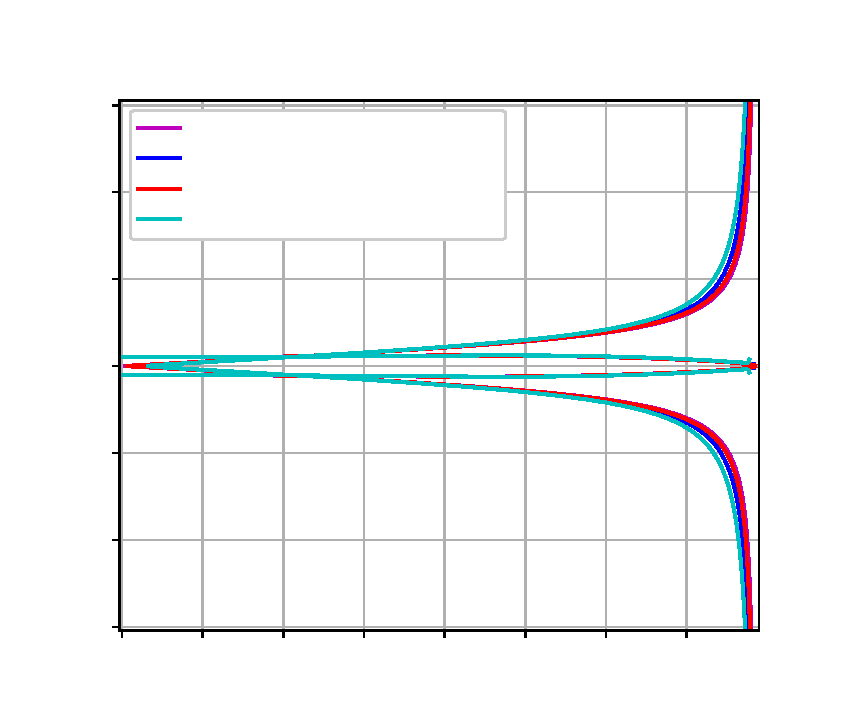
\includegraphics[width=\unitlength]{imagesbat/bat1p.eps}}%
    \put(0.10764293,0.05){\color[rgb]{0,0,0}\makebox(0,0)[lb]{\smash{0.0}}}%
    \put(0.20539672,0.05){\color[rgb]{0,0,0}\makebox(0,0)[lb]{\smash{0.2}}}%
    \put(0.30314899,0.05){\color[rgb]{0,0,0}\makebox(0,0)[lb]{\smash{0.4}}}%
    \put(0.40090404,0.05){\color[rgb]{0,0,0}\makebox(0,0)[lb]{\smash{0.6}}}%
    \put(0.49865657,0.05){\color[rgb]{0,0,0}\makebox(0,0)[lb]{\smash{0.8}}}%
    \put(0.59641162,0.05){\color[rgb]{0,0,0}\makebox(0,0)[lb]{\smash{1.0}}}%
    \put(0.69416414,0.05){\color[rgb]{0,0,0}\makebox(0,0)[lb]{\smash{1.2}}}%
    \put(0.79191667,0.05){\color[rgb]{0,0,0}\makebox(0,0)[lb]{\smash{1.4}}}%
    \put(0.05,0.08659355){\color[rgb]{0,0,0}\makebox(0,0)[lb]{\smash{-15}}}%
    \put(0.05,0.19199405){\color[rgb]{0,0,0}\makebox(0,0)[lb]{\smash{-10}}}%
    \put(0.07,0.29739355){\color[rgb]{0,0,0}\makebox(0,0)[lb]{\smash{-5}}}%
    \put(0.09,0.40279506){\color[rgb]{0,0,0}\makebox(0,0)[lb]{\smash{0}}}%
    \put(0.085,0.50819405){\color[rgb]{0,0,0}\makebox(0,0)[lb]{\smash{5}}}%
    \put(0.065,0.61359557){\color[rgb]{0,0,0}\makebox(0,0)[lb]{\smash{10}}}%
    \put(0.067,0.71899456){\color[rgb]{0,0,0}\makebox(0,0)[lb]{\smash{15}}}%
    \put(0.03065808,0.39910819){\color[rgb]{0,0,0}\rotatebox{90}{\makebox(0,0)[lb]{\smash{$\hat{\omega_0}$}}}}%
    \put(0.21843434,0.69249708){\color[rgb]{0,0,0}\makebox(0,0)[lb]{\smash{\footnotesize $R=1.0m, r_2=1cm$}}}%
    \put(0.21843434,0.65544658){\color[rgb]{0,0,0}\makebox(0,0)[lb]{\smash{\footnotesize$R=1.0m, r_2=5cm$}}}%
    \put(0.21843434,0.61839607){\color[rgb]{0,0,0}\makebox(0,0)[lb]{\smash{\footnotesize$R=0.5m, r_2=1cm $}}}%
    \put(0.21843434,0.58134557){\color[rgb]{0,0,0}\makebox(0,0)[lb]{\smash{\footnotesize$R=0.5m, r_2=5cm $}}}%
    \put(0.42,0.0){\color[rgb]{0,0,0}\makebox(0,0)[lb]{\smash{ $\theta_0 (rad)$}}}%
    \put(0.49865657,0.25){\color[rgb]{0,0,0}\makebox(0,0)[lb]{\smash{stable}}}%
    \put(0.49865657,0.5){\color[rgb]{0,0,0}\makebox(0,0)[lb]{\smash{stable}}}%
    \put(0.6,0.40279506){\color[rgb]{0,0,0}\makebox(0,0)[lb]{\smash{instable}}}%
  \end{picture}%
\endgroup%

\def\svgwidth{250}
%% Creator: Inkscape inkscape 0.92.2, www.inkscape.org
%% PDF/EPS/PS + LaTeX output extension by Johan Engelen, 2010
%% Accompanies image file 'bat2p.eps' (pdf, eps, ps)
%%
%% To include the image in your LaTeX document, write
%%   \input{<filename>.pdf_tex}
%%  instead of
%%   \includegraphics{<filename>.pdf}
%% To scale the image, write
%%   \def\svgwidth{<desired width>}
%%   \input{<filename>.pdf_tex}
%%  instead of
%%   \includegraphics[width=<desired width>]{<filename>.pdf}
%%
%% Images with a different path to the parent latex file can
%% be accessed with the `import' package (which may need to be
%% installed) using
%%   \usepackage{import}
%% in the preamble, and then including the image with
%%   \import{<path to file>}{<filename>.pdf_tex}
%% Alternatively, one can specify
%%   \graphicspath{{<path to file>/}}
%% 
%% For more information, please see info/svg-inkscape on CTAN:
%%   http://tug.ctan.org/tex-archive/info/svg-inkscape
%%
\begingroup%
  \makeatletter%
  \providecommand\color[2][]{%
    \errmessage{(Inkscape) Color is used for the text in Inkscape, but the package 'color.sty' is not loaded}%
    \renewcommand\color[2][]{}%
  }%
  \providecommand\transparent[1]{%
    \errmessage{(Inkscape) Transparency is used (non-zero) for the text in Inkscape, but the package 'transparent.sty' is not loaded}%
    \renewcommand\transparent[1]{}%
  }%
  \providecommand\rotatebox[2]{#2}%
  \ifx\svgwidth\undefined%
    \setlength{\unitlength}{395.9999901bp}%
    \ifx\svgscale\undefined%
      \relax%
    \else%
      \setlength{\unitlength}{\unitlength * \real{\svgscale}}%
    \fi%
  \else%
    \setlength{\unitlength}{\svgwidth}%
  \fi%
  \global\let\svgwidth\undefined%
  \global\let\svgscale\undefined%
  \makeatother%
  \begin{picture}(1,0.833939)%
    \put(0,0){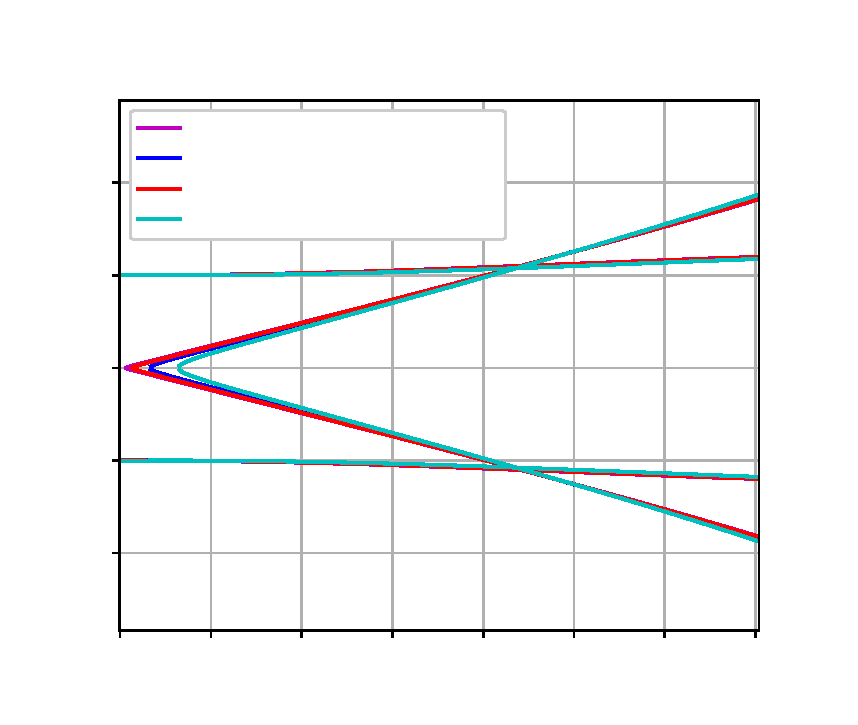
\includegraphics[width=\unitlength]{imagesbat/bat2p.eps}}%
    \put(0.10533056,0.05){\color[rgb]{0,0,0}\makebox(0,0)[lb]{\smash{0.0}}}%
    \put(0.21535177,0.05){\color[rgb]{0,0,0}\makebox(0,0)[lb]{\smash{0.1}}}%
    \put(0.32537374,0.05){\color[rgb]{0,0,0}\makebox(0,0)[lb]{\smash{0.2}}}%
    \put(0.43539394,0.05){\color[rgb]{0,0,0}\makebox(0,0)[lb]{\smash{0.3}}}%
    \put(0.54541414,0.05){\color[rgb]{0,0,0}\makebox(0,0)[lb]{\smash{0.4}}}%
    \put(0.65543434,0.05){\color[rgb]{0,0,0}\makebox(0,0)[lb]{\smash{0.5}}}%
    \put(0.76545707,0.05){\color[rgb]{0,0,0}\makebox(0,0)[lb]{\smash{0.6}}}%
    \put(0.87547727,0.05){\color[rgb]{0,0,0}\makebox(0,0)[lb]{\smash{0.7}}}%
    \put(0.035,0.17609683){\color[rgb]{0,0,0}\makebox(0,0)[lb]{\smash{-1.0}}}%
    \put(0.04,0.28830516){\color[rgb]{0,0,0}\makebox(0,0)[lb]{\smash{-0.5}}}%
    \put(0.05,0.40051223){\color[rgb]{0,0,0}\makebox(0,0)[lb]{\smash{0.0}}}%
    \put(0.05,0.5127193){\color[rgb]{0,0,0}\makebox(0,0)[lb]{\smash{0.5}}}%
    \put(0.05,0.62492637){\color[rgb]{0,0,0}\makebox(0,0)[lb]{\smash{1.0}}}%
    \put(0.03065808,0.39910819){\color[rgb]{0,0,0}\rotatebox{90}{\makebox(0,0)[lb]{\smash{$\hat{\omega_0}$}}}}%
    \put(0.21843434,0.69249708){\color[rgb]{0,0,0}\makebox(0,0)[lb]{\smash{\footnotesize $R=1.0m, r_2=1cm$}}}%
    \put(0.21843434,0.65544658){\color[rgb]{0,0,0}\makebox(0,0)[lb]{\smash{\footnotesize$R=1.0m, r_2=5cm$}}}%
    \put(0.21843434,0.61839607){\color[rgb]{0,0,0}\makebox(0,0)[lb]{\smash{\footnotesize$R=0.5m, r_2=1cm $}}}%
    \put(0.21843434,0.58134557){\color[rgb]{0,0,0}\makebox(0,0)[lb]{\smash{\footnotesize$R=0.5m, r_2=5cm $}}}%
    \put(0.42,0.0){\color[rgb]{0,0,0}\makebox(0,0)[lb]{\smash{ $\theta_0 (rad)$}}}%
    \put(0.35,0.18609683){\color[rgb]{0,0,0}\makebox(0,0)[lb]{\smash{\footnotesize stable}}}%
    \put(0.65543434,0.40051223){\color[rgb]{0,0,0}\makebox(0,0)[lb]{\smash{\footnotesize instable}}}%
    \put(0.13,0.34){\color[rgb]{0,0,0}\makebox(0,0)[lb]{\smash{\footnotesize instable en}}}%
    \put(0.13,0.31){\color[rgb]{0,0,0}\makebox(0,0)[lb]{\smash{\footnotesize cas de perturbation}}}%
  \end{picture}%
\endgroup%

\caption{Carte de stabilité. Les frontières déterminent l'existence d'une position d'équilibre dynamique pour chaque couple ($\theta_0,\hat{\omega_0}$), où $\hat{\omega_0}$ correspond à la vitesse de rotation adimensionnelle, $\hat{\omega_0}=\omega_0 \sqrt{\dfrac{R+r_2}{g}}$}
\end{figure}

             % Second thème (Doctorat) ou "Résultats théoriques et expérimentaux" (Maîtrise).
\Chapter{ETUDE DE LA RESISTANCE D'UNE ROUE CYR}\label{sec:Theme3}

\section{Masse minimale}

Réduire la masse de la roue Cyr revient à enlever de la matière. Il existe donc une masse minimale en dessous de laquelle la roue ne pourra pas résister aux contraintes induites par le poids de l'utilisateur.

\begin{itemize}
    \item On commence par calculer les contraintes lorsque la roue est comprimée par une force $F$: La contrainte dans l'arrête extérieure s'exprime $\sigma_i=k_i\sigma$ \cite{roark},
    où sigma est la contrainte calculée pour une poutre droite: $\sigma=\frac{Mr_2}{I_z}$, avec $I_z=\frac{\pi}{2}(r_2^4-r_1^4)$ et $M=\frac{\pi}{4}FR$.
    D'après les formules du livre de Roark, $k_i$ s'exprime $k_i=\frac{1}{4\beta}\frac{1-\beta}{\frac{R_c}{r_2}-1}[1+(\frac{r_1}{r_2})^2]$ avec $\beta=\frac{1}{2}[\frac{2R_c}{r_2}-\sqrt{(\frac{R_c}{r_2})^2-1}-\sqrt{(\frac{R_c}{r_2})^2-(\frac{r_1}{r_2})^2}]$ 
    \item Il ne reste plus qu'à déterminer le rayon de courbure de la roue comprimée, comme illustré sur la figure \ref{fig:ellr}: $R_c=\frac{a_r^2}{b_r}$, $a_r$ et $b_r$ étant respectivement les demi grand axe et demi petit axe de l'ellipse que devient la roue lorsqu'elle est comprimée.\\
    
    \begin{figure}[htb]
    \centering
    %% Creator: Inkscape inkscape 0.92.2, www.inkscape.org
%% PDF/EPS/PS + LaTeX output extension by Johan Engelen, 2010
%% Accompanies image file 'ellipse.eps' (pdf, eps, ps)
%%
%% To include the image in your LaTeX document, write
%%   \input{<filename>.pdf_tex}
%%  instead of
%%   \includegraphics{<filename>.pdf}
%% To scale the image, write
%%   \def\svgwidth{<desired width>}
%%   \input{<filename>.pdf_tex}
%%  instead of
%%   \includegraphics[width=<desired width>]{<filename>.pdf}
%%
%% Images with a different path to the parent latex file can
%% be accessed with the `import' package (which may need to be
%% installed) using
%%   \usepackage{import}
%% in the preamble, and then including the image with
%%   \import{<path to file>}{<filename>.pdf_tex}
%% Alternatively, one can specify
%%   \graphicspath{{<path to file>/}}
%% 
%% For more information, please see info/svg-inkscape on CTAN:
%%   http://tug.ctan.org/tex-archive/info/svg-inkscape
%%
\begingroup%
  \makeatletter%
  \providecommand\color[2][]{%
    \errmessage{(Inkscape) Color is used for the text in Inkscape, but the package 'color.sty' is not loaded}%
    \renewcommand\color[2][]{}%
  }%
  \providecommand\transparent[1]{%
    \errmessage{(Inkscape) Transparency is used (non-zero) for the text in Inkscape, but the package 'transparent.sty' is not loaded}%
    \renewcommand\transparent[1]{}%
  }%
  \providecommand\rotatebox[2]{#2}%
  \ifx\svgwidth\undefined%
    \setlength{\unitlength}{318.40595442bp}%
    \ifx\svgscale\undefined%
      \relax%
    \else%
      \setlength{\unitlength}{\unitlength * \real{\svgscale}}%
    \fi%
  \else%
    \setlength{\unitlength}{\svgwidth}%
  \fi%
  \global\let\svgwidth\undefined%
  \global\let\svgscale\undefined%
  \makeatother%
  \begin{picture}(1,0.51062056)%
    \put(0,0){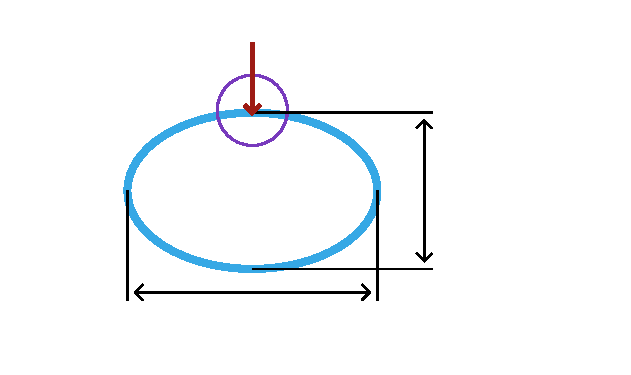
\includegraphics[width=\unitlength]{images_contraintes/ellipse.eps}}%
    \put(0.69807629,0.26119896){\color[rgb]{0,0,0}\makebox(0,0)[lb]{\smash{$2a_r$}}}%
    \put(0.380830868,0.06042804){\color[rgb]{0,0,0}\makebox(0,0)[lb]{\smash{$2b_r$}}}%
    \put(0.34402215,0.52558617){\color[rgb]{0.61568627,0.10588235,0.07843137}\makebox(0,0)[lb]{\smash{$F$}}}%
    \put(0.45664975,0.45341089){\color[rgb]{0.47058824,0.22745098,0.74117647}\makebox(0,0)[lb]{\smash{zone où les contraintes sont maximales}}}%
    \put(0.82651502,0.40252801){\color[rgb]{0,0,0}\makebox(0,0)[lb]{\smash{}}}%
  \end{picture}%
\endgroup%

    \caption{Représentation schématique d'un tore plié par une force de compression F. Il devient une ellipse de demi grand axe $a_r$ et de demi petit axe $b_r$. La zone où les contraintes sont maximales correspond à l'endroit où la force est appliquée.}
    \label{fig:ellr}
    \end{figure}
    
\begin{itemize}
    \item Pour calculer $a_r$ et $b_r$, on utilise les formules du livre de Roark qui donnent les variations de diamètre horizontal $\Delta D_h$ et vertical $\Delta D_v$ d'une anneau comprimé selon son diamètre avec une force $F$, et on aura ainsi $a_r=R+\frac{\Delta D_h}{2}$ et $b_r=R+\frac{\Delta D_v}{2}$.
    \item D'après les formules de Roark, $\Delta D_h=\frac{FR^3}{EI}(\frac{1}{2}(1+\frac{I}{AR^2}+\frac{2EI}{GAR^2})-1+\frac{2}{/pi}(1-\frac{I}{AR^2})^2)$ et $\Delta D_v=-\frac{FR^3}{EI}(\frac{\pi}{4}(1-\frac{I}{AR^2}+\frac{2EI}{GAR^2})-\frac{2}{/pi}(1-\frac{I}{AR^2})^2)$, où $A$ est l'aire de section, $E$, le module de Young, $G$, le module de cisaillement, $R$, le rayon médian de la roue, et $I$ le moment de section quadratique selon l'axe principal perpendiculaire au plan de la roue.
    \item En implémentant numériquement les équations ci-dessus, on est capable de calculer les contraintes maximales auxquelles sera soumise la roue pour une force de compression $F$ donnée. Pour $F=900N$, en fixant $r_2$ et en faisant varier $r_1$ de $0$ à $r_2$, on est capable de tracer les contraintes maximales, en fonction de la masse de la roue, $m_r=2\pi\rho A R$. Comme l'illustre la figure-\ref{fig:mmin1} ci-dessous, il est alors possible de déterminer la masse à partir de laquelle les contraintes passent sous le seuil de $63 MPa$, et donc à partir de laquelle il y a rupture.
    
\end{itemize}


\begin{figure}[htb]
\centering
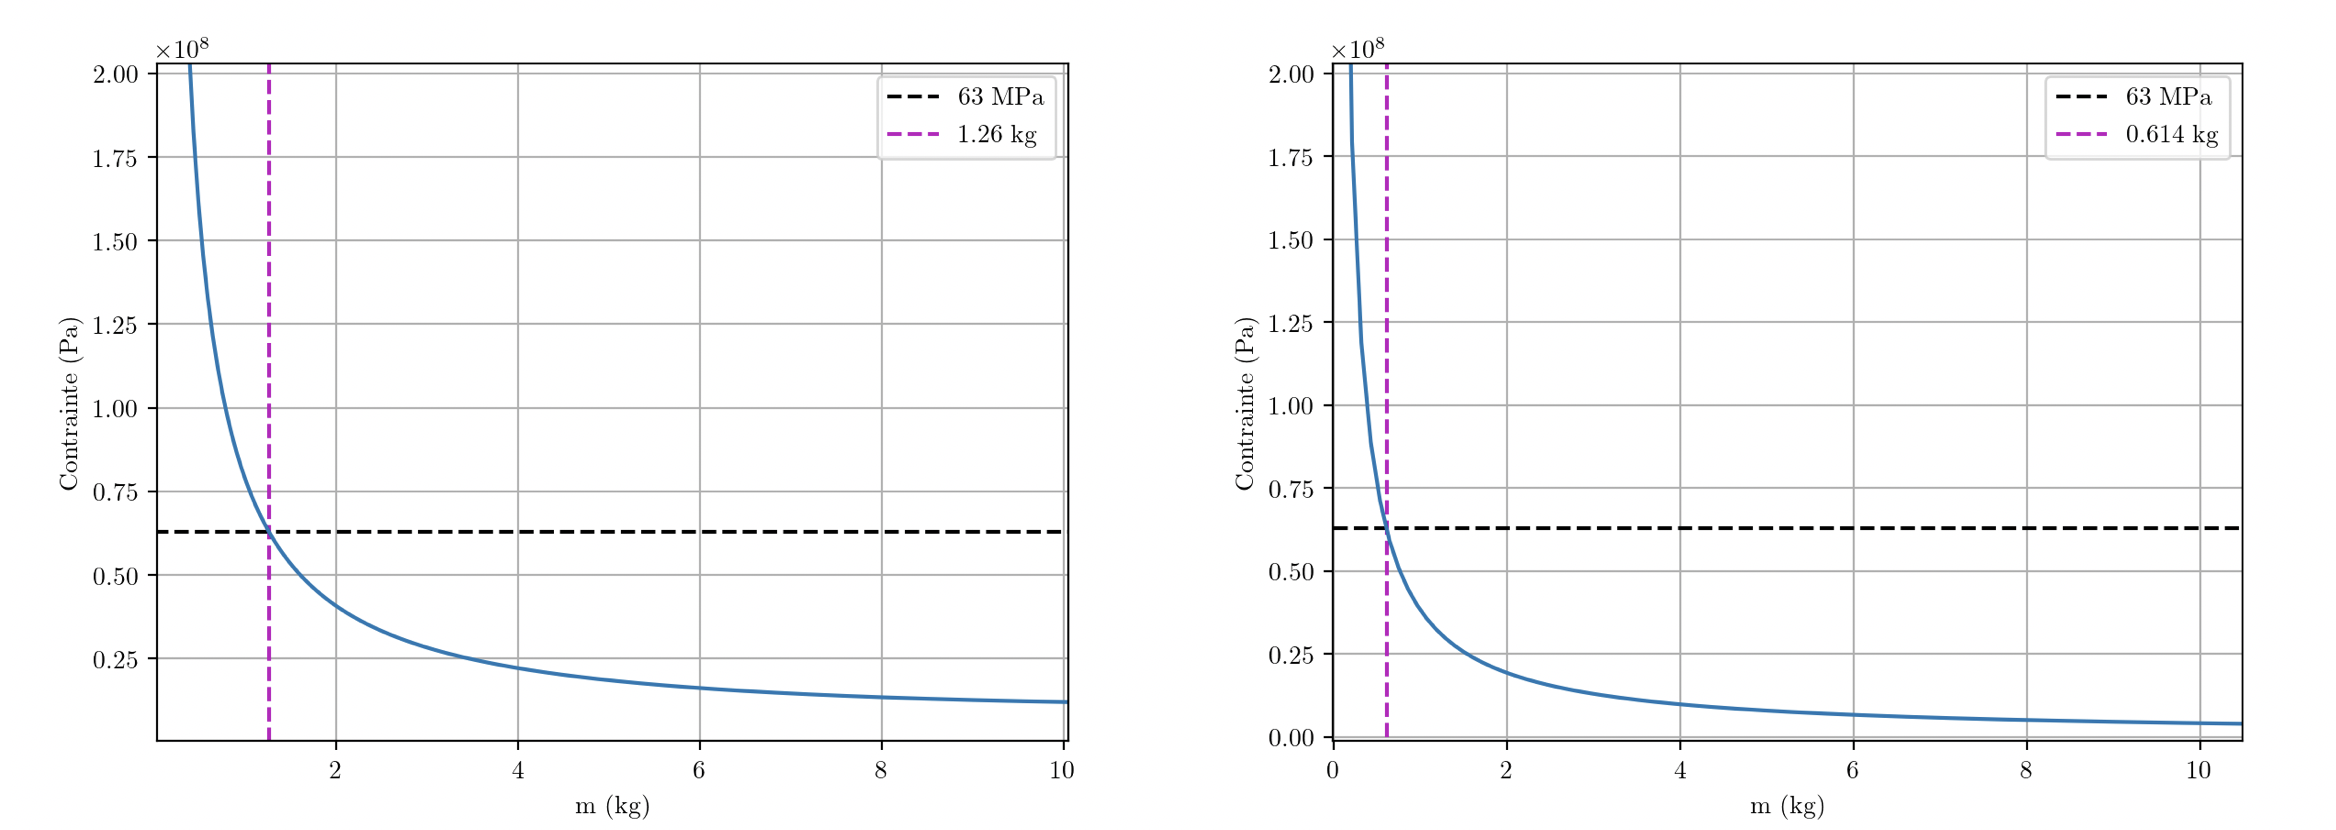
\includegraphics[width=7in]{images_2ddl/mmin1.png}
\caption{Contraintes maximales dans la roue en fonction de sa masse, la courbe de gauche correspond à un rayon de section externe $r_2=2.5 cm$ et un rayon de section interne $r_1$ variant de $0.0$ à $2.49 cm$. La courbe de droite correspond à à $r_2=5.0 cm$ et $r_1$ variant de $0.0$ à $4.99 cm$}
\label{fig:mmin1}
\end{figure}


\begin{itemize}
    \item On peut donc implémenter ce procédé numériquement pour déterminer cette valeur minimale de la masse pour en fonction de $r_2$. Le resultat de l'implémentation est présenté à la figure-\ref{fig:mmin2} ci-dessous. 
\end{itemize}


\begin{figure}[htb]
\centering
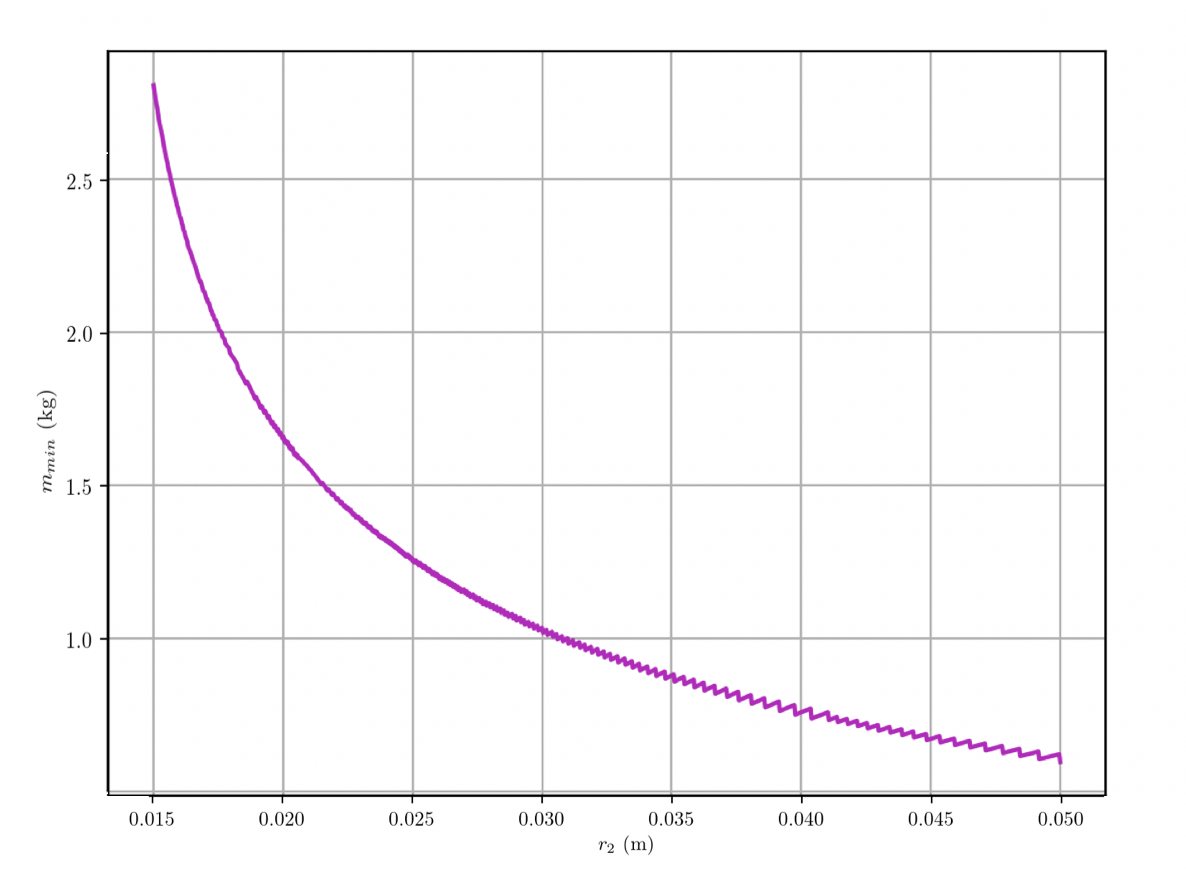
\includegraphics[width=4in]{images_2ddl/mmin2.png}
\caption{Masse minimale de la roue en fonction de $r_2$}
\label{fig:mmin2}
\end{figure}


\item Pour ce qui suit, $r_2$ sera fixé à $1.75 cm$, la masse minimale sera donc $2.0 kg$
\end{itemize}
             % Troisième thème (Doctorat) ou effacez ce fichier si vous êtes à la Maîtrise.
\Chapter{CONCLUSION}\label{sec:Conclusion}
Texte / Text.

%%
%%  SYNTHESE DES TRAVAUX / SUMMARY OF WORKS
%%
\section{Synthèse des travaux / Summary of Works}
Texte / Text.

%%
%%  LIMITATIONS
%%
\section{Limitations de la solution proposée / Limitations}\label{sec:Limitations}

%%
%%  AMELIORATIONS FUTURES *-/ FUTURE RESEARCH
%%
\section{Améliorations futures / Future Research}
Texte / Text.
         % Conclusion.
%\backmatter
\ifthenelse{\equal{\Langue}{english}}{
	\renewcommand\bibname{REFERENCES}
	\bibliography{Document}
	\bibliographystyle{IEEEtran}			% Bibliography style. 
}{
	\renewcommand\bibname{RÉFÉRENCES}
	\bibliography{Document}
	\bibliographystyle{IEEEtran-francais}    % Style de la bibliographie. 
}
%
\ifthenelse{\equal{\AnnexesPresentes}{O}}{
	\appendix%
	\newcommand{\Annexe}[1]{\annexe{#1}\setcounter{figure}{0}\setcounter{table}{0}\setcounter{footnote}{0}}%
	%%
%%  Annexes
%%
%%  Note: Ne pas modifier la ligne ci-dessous. / Do not modify the following line.
\ifthenelse{\equal{\Langue}{english}}{
	\addcontentsline{toc}{compteur}{APPENDICES}
}{
	\addcontentsline{toc}{compteur}{ANNEXES}
}
%%
%%
%%  Toutes les annexes doivent être inclues dans ce document
%%  les unes à la suite des autres.
%%  All annexes must be included in this document one after the other.
\Annexe{Démo}
Texte de l'annexe A\@. Remarquez que la phrase précédente se termine
par une lettre majuscule suivie d'un point. On indique explicitement
cette situation à \LaTeX{} afin que ce dernier ajuste correctement
l'espacement entre le point final de la phrase et le début de la
phrase suivante.


\begin{landscape}
\Annexe{Encore une annexe / Another Appendix}
Texte de l'annexe B\@ en mode «landscape».
\end{landscape}

\Annexe{Une dernière annexe / The Last Appendix}
Texte de l'annexe C\@.
}
{}
\end{document}
